%        File: dev.tex 
%     Created: dom ago 27 23:42  2006 C
% Last Change: lun dic 11 10:46  2006 C
%
% NOTA: Las imágenes se ven como el culo. Comento. No s'e si por el puerto paralelo, por CUPS, por la impresora o por qu'e, pero salen con un grano muy grueso y ni siquiera se distingue el texto en algunas.
% NOTA: Desconozco si este es la última versión del documento. Acabar'e meti'endolo el el CVS para sincronizar las dos o tres copias que tengo de este archivo.

\documentclass[a4paper]{article}
\usepackage{listings}
\usepackage{color}
\usepackage{ucs}
\usepackage[utf8]{inputenc}
\usepackage[spanish,activeacute]{babel}
\usepackage{fancyhdr}
\usepackage{amsmath}
\usepackage[dvips]{graphicx}
\usepackage{tocbibind}
\usepackage{longtable}
\pagestyle{fancy}
\usepackage{color,soul}
\usepackage{anysize} % Soporte para el comando \marginsize
\marginsize{2cm}{2cm}{2cm}{2cm}


\setcounter{secnumdepth}{3}
\setcounter{tocdepth}{3} 

% Símbolo euro a manopla
\def\euro{\,\hbox{\raise .36em\hbox to0pt{\vrule height0.5pt%
          width.55em depth0pt\hss}%
          \raise .25em\hbox to0pt{\vrule height0.5pt width.5em%
          depth0pt\hss}\hskip.02em\sf C}}  

% Redistribución de figuras flotantes más flexible
\setcounter{topnumber}{4}
\setcounter{bottomnumber}{4}
\setcounter{totalnumber}{4}
\setcounter{dbltopnumber}{4}
\renewcommand{\topfraction}{.97}
\renewcommand{\bottomfraction}{.97}
\renewcommand{\textfraction}{.03}
\renewcommand{\floatpagefraction}{.9}
\renewcommand{\dbltopfraction}{.97}
\renewcommand{\dblfloatpagefraction}{.9}
\setlength{\floatsep}{12pt plus 6pt minus 4pt}
\setlength{\textfloatsep}{15pt plus 8pt minus 5pt}
\setlength{\intextsep}{12pt plus 6pt minus 4pt}
\setlength{\dblfloatsep}{12pt plus 6pt minus 4pt}
\setlength{\dbltextfloatsep}{15pt plus 8pt minus 5pt}


\usepackage{calc}
\usepackage{graphicx}
\newcommand{\marginalnote}[1]{\mbox{}\marginpar{\raggedright\hspace{0pt}#1}}

% \iconomargen{alto}{fichero}
% alto: altura en número de líneas de texto a ocupar
% fichero: ruta y nombre de fichero gráfico (sólo formatos compatibles)
%          que contiene el icono a mostrar en el margen
\newcommand{\iconomargen}[2]{%
  \marginalnote{%
    \parbox[t][\baselineskip * (#1-1)][b]{\marginparwidth}{%
      \includegraphics[height=\baselineskip * (#1-1) + 1.5ex]{#2}%
    }
  }
}


\begin{document}
    % Aquí el título
    \title{\Huge ./doc} 

  \begin{figure}
    \begin{center}
      
\includegraphics[width=6cm]{logo}
    \end{center}
  \end{figure}
  
    \author{\large \textit{Francisco José Rodríguez Bogado} (\texttt{rodriguez.bogado@gmail.com})} 
    \date{\Large \today}
    \maketitle
    

%\iconomargen{5}{inn14}
  
    % Resumen 
    \begin{abstract}
    Documentación y memorándum de desarrollo de \Large \textbf{Geotex-INN~v1.9.31b}.
    % ¿Memoria, memorándum, simplemente documentación, las dos cosas, LAS TRES?
    \end{abstract}

  \begin{figure}
    \begin{flushright}
      
\includegraphics[width=1.5cm]{inn14}
    \end{flushright}
  \end{figure}
  
    \newpage

%Aquí va la cabecera
\renewcommand{\headwidth}{\textwidth}
\renewcommand{\headrulewidth}{0.4pt}
\renewcommand{\footrulewidth}{0.4pt}
\lhead{ginn}
\chead{}
\rhead{\bfseries Documentación de desarrollo}
\lfoot{\em ./doc/dev} 
\rfoot{\thepage}
\cfoot{}
    
    % El índice
    \tableofcontents
    \listoffigures
    \newpage

    % Y a empezar a escribir
    \section{Licencia}

\begin{center}
{\parindent 0in
The GNU General Public License

Version 2, June 1991

Copyright \copyright\ 1989, 1991 Free Software Foundation, Inc.

\bigskip

51 Franklin St, Fifth Floor, Boston, MA  02110-1301, USA

\bigskip

Everyone is permitted to copy and distribute verbatim copies
of this license document, but changing it is not allowed.
}
\end{center}

%\renewcommand{\abstractname}{Preamble}
%\begin{abstract}
%The licenses for most software are designed to take away your freedom to
%share and change it.  By contrast, the GNU General Public License is
%intended to guarantee your freedom to share and change free software---to
%make sure the software is free for all its users.  This General Public
%License applies to most of the Free Software Foundation's software and to
%any other program whose authors commit to using it.  (Some other Free
%Software Foundation software is covered by the GNU Library General Public
%License instead.)  You can apply it to your programs, too.
%
%When we speak of free software, we are referring to freedom, not price.
%Our General Public Licenses are designed to make sure that you have the
%freedom to distribute copies of free software (and charge for this service
%if you wish), that you receive source code or can get it if you want it,
%that you can change the software or use pieces of it in new free programs;
%and that you know you can do these things.
%
%To protect your rights, we need to make restrictions that forbid anyone to
%deny you these rights or to ask you to surrender the rights.  These
%restrictions translate to certain responsibilities for you if you
%distribute copies of the software, or if you modify it.
%
%For example, if you distribute copies of such a program, whether gratis or
%for a fee, you must give the recipients all the rights that you have.  You
%must make sure that they, too, receive or can get the source code.  And
%you must show them these terms so they know their rights.
%
%We protect your rights with two steps: (1) copyright the software, and (2)
%offer you this license which gives you legal permission to copy,
%distribute and/or modify the software.
%
%Also, for each author's protection and ours, we want to make certain that
%everyone understands that there is no warranty for this free software.  If
%the software is modified by someone else and passed on, we want its
%recipients to know that what they have is not the original, so that any
%problems introduced by others will not reflect on the original authors'
%reputations.
%
%Finally, any free program is threatened constantly by software patents.
%We wish to avoid the danger that redistributors of a free program will
%individually obtain patent licenses, in effect making the program
%proprietary.  To prevent this, we have made it clear that any patent must
%be licensed for everyone's free use or not licensed at all.
%
%The precise terms and conditions for copying, distribution and
%modification follow.
%\end{abstract}

\begin{center}
{\Large \sc GNU General Public License
\\\vspace{3mm}Terms and Conditions For Copying, Distribution and Modification}
\end{center}


\begin{enumerate}

\addtocounter{enumi}{-1}

\item 

This License applies to any program or other work which contains a notice
placed by the copyright holder saying it may be distributed under the
terms of this General Public License.  The ``Program'', below, refers to
any such program or work, and a ``work based on the Program'' means either
the Program or any derivative work under copyright law: that is to say, a
work containing the Program or a portion of it, either verbatim or with
modifications and/or translated into another language.  (Hereinafter,
translation is included without limitation in the term ``modification''.)
Each licensee is addressed as ``you''.

Activities other than copying, distribution and modification are not
covered by this License; they are outside its scope.  The act of
running the Program is not restricted, and the output from the Program
is covered only if its contents constitute a work based on the
Program (independent of having been made by running the Program).
Whether that is true depends on what the Program does.

\item You may copy and distribute verbatim copies of the Program's source
  code as you receive it, in any medium, provided that you conspicuously
  and appropriately publish on each copy an appropriate copyright notice
  and disclaimer of warranty; keep intact all the notices that refer to
  this License and to the absence of any warranty; and give any other
  recipients of the Program a copy of this License along with the Program.

You may charge a fee for the physical act of transferring a copy, and you
may at your option offer warranty protection in exchange for a fee.

\item

You may modify your copy or copies of the Program or any portion
of it, thus forming a work based on the Program, and copy and
distribute such modifications or work under the terms of Section 1
above, provided that you also meet all of these conditions:

\begin{enumerate}

\item 

You must cause the modified files to carry prominent notices stating that
you changed the files and the date of any change.

\item

You must cause any work that you distribute or publish, that in
whole or in part contains or is derived from the Program or any
part thereof, to be licensed as a whole at no charge to all third
parties under the terms of this License.

\item
If the modified program normally reads commands interactively
when run, you must cause it, when started running for such
interactive use in the most ordinary way, to print or display an
announcement including an appropriate copyright notice and a
notice that there is no warranty (or else, saying that you provide
a warranty) and that users may redistribute the program under
these conditions, and telling the user how to view a copy of this
License.  (Exception: if the Program itself is interactive but
does not normally print such an announcement, your work based on
the Program is not required to print an announcement.)

\end{enumerate}


These requirements apply to the modified work as a whole.  If
identifiable sections of that work are not derived from the Program,
and can be reasonably considered independent and separate works in
themselves, then this License, and its terms, do not apply to those
sections when you distribute them as separate works.  But when you
distribute the same sections as part of a whole which is a work based
on the Program, the distribution of the whole must be on the terms of
this License, whose permissions for other licensees extend to the
entire whole, and thus to each and every part regardless of who wrote it.

Thus, it is not the intent of this section to claim rights or contest
your rights to work written entirely by you; rather, the intent is to
exercise the right to control the distribution of derivative or
collective works based on the Program.

In addition, mere aggregation of another work not based on the Program
with the Program (or with a work based on the Program) on a volume of
a storage or distribution medium does not bring the other work under
the scope of this License.

\item
You may copy and distribute the Program (or a work based on it,
under Section 2) in object code or executable form under the terms of
Sections 1 and 2 above provided that you also do one of the following:

\begin{enumerate}

\item

Accompany it with the complete corresponding machine-readable
source code, which must be distributed under the terms of Sections
1 and 2 above on a medium customarily used for software interchange; or,

\item

Accompany it with a written offer, valid for at least three
years, to give any third party, for a charge no more than your
cost of physically performing source distribution, a complete
machine-readable copy of the corresponding source code, to be
distributed under the terms of Sections 1 and 2 above on a medium
customarily used for software interchange; or,

\item

Accompany it with the information you received as to the offer
to distribute corresponding source code.  (This alternative is
allowed only for noncommercial distribution and only if you
received the program in object code or executable form with such
an offer, in accord with Subsection b above.)

\end{enumerate}


The source code for a work means the preferred form of the work for
making modifications to it.  For an executable work, complete source
code means all the source code for all modules it contains, plus any
associated interface definition files, plus the scripts used to
control compilation and installation of the executable.  However, as a
special exception, the source code distributed need not include
anything that is normally distributed (in either source or binary
form) with the major components (compiler, kernel, and so on) of the
operating system on which the executable runs, unless that component
itself accompanies the executable.

If distribution of executable or object code is made by offering
access to copy from a designated place, then offering equivalent
access to copy the source code from the same place counts as
distribution of the source code, even though third parties are not
compelled to copy the source along with the object code.

\item
You may not copy, modify, sublicense, or distribute the Program
except as expressly provided under this License.  Any attempt
otherwise to copy, modify, sublicense or distribute the Program is
void, and will automatically terminate your rights under this License.
However, parties who have received copies, or rights, from you under
this License will not have their licenses terminated so long as such
parties remain in full compliance.

\item
You are not required to accept this License, since you have not
signed it.  However, nothing else grants you permission to modify or
distribute the Program or its derivative works.  These actions are
prohibited by law if you do not accept this License.  Therefore, by
modifying or distributing the Program (or any work based on the
Program), you indicate your acceptance of this License to do so, and
all its terms and conditions for copying, distributing or modifying
the Program or works based on it.

\item
Each time you redistribute the Program (or any work based on the
Program), the recipient automatically receives a license from the
original licensor to copy, distribute or modify the Program subject to
these terms and conditions.  You may not impose any further
restrictions on the recipients' exercise of the rights granted herein.
You are not responsible for enforcing compliance by third parties to
this License.

\item
If, as a consequence of a court judgment or allegation of patent
infringement or for any other reason (not limited to patent issues),
conditions are imposed on you (whether by court order, agreement or
otherwise) that contradict the conditions of this License, they do not
excuse you from the conditions of this License.  If you cannot
distribute so as to satisfy simultaneously your obligations under this
License and any other pertinent obligations, then as a consequence you
may not distribute the Program at all.  For example, if a patent
license would not permit royalty-free redistribution of the Program by
all those who receive copies directly or indirectly through you, then
the only way you could satisfy both it and this License would be to
refrain entirely from distribution of the Program.

If any portion of this section is held invalid or unenforceable under
any particular circumstance, the balance of the section is intended to
apply and the section as a whole is intended to apply in other
circumstances.

It is not the purpose of this section to induce you to infringe any
patents or other property right claims or to contest validity of any
such claims; this section has the sole purpose of protecting the
integrity of the free software distribution system, which is
implemented by public license practices.  Many people have made
generous contributions to the wide range of software distributed
through that system in reliance on consistent application of that
system; it is up to the author/donor to decide if he or she is willing
to distribute software through any other system and a licensee cannot
impose that choice.

This section is intended to make thoroughly clear what is believed to
be a consequence of the rest of this License.

\item
If the distribution and/or use of the Program is restricted in
certain countries either by patents or by copyrighted interfaces, the
original copyright holder who places the Program under this License
may add an explicit geographical distribution limitation excluding
those countries, so that distribution is permitted only in or among
countries not thus excluded.  In such case, this License incorporates
the limitation as if written in the body of this License.

\item
The Free Software Foundation may publish revised and/or new versions
of the General Public License from time to time.  Such new versions will
be similar in spirit to the present version, but may differ in detail to
address new problems or concerns.

Each version is given a distinguishing version number.  If the Program
specifies a version number of this License which applies to it and ``any
later version'', you have the option of following the terms and conditions
either of that version or of any later version published by the Free
Software Foundation.  If the Program does not specify a version number of
this License, you may choose any version ever published by the Free Software
Foundation.

\item
If you wish to incorporate parts of the Program into other free
programs whose distribution conditions are different, write to the author
to ask for permission.  For software which is copyrighted by the Free
Software Foundation, write to the Free Software Foundation; we sometimes
make exceptions for this.  Our decision will be guided by the two goals
of preserving the free status of all derivatives of our free software and
of promoting the sharing and reuse of software generally.

\begin{center}
{\Large\sc
No Warranty
}
\end{center}

\item
{\sc Because the program is licensed free of charge, there is no warranty
for the program, to the extent permitted by applicable law.  Except when
otherwise stated in writing the copyright holders and/or other parties
provide the program ``as is'' without warranty of any kind, either expressed
or implied, including, but not limited to, the implied warranties of
merchantability and fitness for a particular purpose.  The entire risk as
to the quality and performance of the program is with you.  Should the
program prove defective, you assume the cost of all necessary servicing,
repair or correction.}

\item
{\sc In no event unless required by applicable law or agreed to in writing
will any copyright holder, or any other party who may modify and/or
redistribute the program as permitted above, be liable to you for damages,
including any general, special, incidental or consequential damages arising
out of the use or inability to use the program (including but not limited
to loss of data or data being rendered inaccurate or losses sustained by
you or third parties or a failure of the program to operate with any other
programs), even if such holder or other party has been advised of the
possibility of such damages.}

\end{enumerate}


\begin{center}
{\Large\sc End of Terms and Conditions}
\end{center}


%\pagebreak[2]
%
%\section*{Appendix: How to Apply These Terms to Your New Programs}
%
%If you develop a new program, and you want it to be of the greatest
%possible use to the public, the best way to achieve this is to make it
%free software which everyone can redistribute and change under these
%terms.
%
%  To do so, attach the following notices to the program.  It is safest to
%  attach them to the start of each source file to most effectively convey
%  the exclusion of warranty; and each file should have at least the
%  ``copyright'' line and a pointer to where the full notice is found.
%
%\begin{quote}
%<one line to give the program's name and a brief idea of what it does.> \\
%Copyright (C) <year>  <name of author> \\
%
%This program is free software; you can redistribute it and/or modify
%it under the terms of the GNU General Public License as published by
%the Free Software Foundation; either version 2 of the License, or
%(at your option) any later version.
%
%This program is distributed in the hope that it will be useful,
%%but WITHOUT ANY WARRANTY; without even the implied warranty of
%MERCHANTABILITY or FITNESS FOR A PARTICULAR PURPOSE.  See the
%GNU General Public License for more details.
%
%You should have received a copy of the GNU General Public License
%along with this program; if not, write to the Free Software
%Foundation, Inc., 51 Franklin St, Fifth Floor, Boston, MA  02110-1301, USA.
%\end{quote}
%
%Also add information on how to contact you by electronic and paper mail.
%
%If the program is interactive, make it output a short notice like this
%when it starts in an interactive mode:
%
%\begin{quote}
%Gnomovision version 69, Copyright (C) <year>  <name of author> \\
%Gnomovision comes with ABSOLUTELY NO WARRANTY; for details type `show w'. \\
%This is free software, and you are welcome to redistribute it
%under certain conditions; type `show c' for details.
%\end{quote}
%
%
%The hypothetical commands {\tt show w} and {\tt show c} should show the
%appropriate parts of the General Public License.  Of course, the commands
%you use may be called something other than {\tt show w} and {\tt show c};
%they could even be mouse-clicks or menu items---whatever suits your
%program.
%
%You should also get your employer (if you work as a programmer) or your
%school, if any, to sign a ``copyright disclaimer'' for the program, if
%necessary.  Here is a sample; alter the names:
%
%\begin{quote}
%Yoyodyne, Inc., hereby disclaims all copyright interest in the program \\
%`Gnomovision' (which makes passes at compilers) written by James Hacker. \\
%
%<signature of Ty Coon>, 1 April 1989 \\
%Ty Coon, President of Vice
%\end{quote}
%
%
%This General Public License does not permit incorporating your program
%into proprietary programs.  If your program is a subroutine library, you
%may consider it more useful to permit linking proprietary applications
%with the library.  If this is what you want to do, use the GNU Library
%General Public License instead of this License.
%
    
    \section{Cr'editos}
        \begin{center}
        \begin{tabular}{r@{:} c @{(}c@{)}}
            Análisis, diseño y desarrollo & Francisco Jos'e Rodríguez Bogado & \texttt{rodriguez.bogado@gmail.com} \\
            Desarrollo                    & Diego Muñoz Escalante            & \texttt{escalant3@gmail.com} \\
            \emph{Third-party}: numerals  & Chema Cort'es                    & \texttt{pych3m4@gmail.com} \\
            \emph{Third-party}: SQLObject & Ian Bicking                      & \texttt{ianb@colorstudy.com} \\
            \emph{Third-party}: Gajim     & Yann Le Boulanger                & \texttt{asterix@lagaule.org} \\
                                          & Nikos Kouremenos                 & \texttt{kourem@gmail.com} \\
                                          & Dimitur Kirov                    & \texttt{dkirov@gmail.com} \\
                                          & Travis Shirk                     & \texttt{travis@pobox.com} \\
            \emph{Third-party}: libgmail  &                                  & \texttt{stas@linux.isbeter.nl} \\
                                          &                                  & \texttt{wdaher@mit.edu} \\
                                          &                                  & \texttt{follower@myrealbox.com} \\
            \emph{Third-party}: XML-RPC   & Yasushi Saito                    & \texttt{yasushi.saito@gmail.com} \\
            \emph{Third-party}: PyChart   & Yasushi Saito                    & \texttt{yasushi.saito@gmail.com} \\
            \emph{Third-party}: Pyconsole & Yevgen Muntyan                   & \texttt{muntyan@math.tamu.edu} \\
            \emph{Artwork}                & Kuswanto                         & \texttt{zeussama@gmail.com} \\
        \end{tabular}
        \end{center}
    \section{Dependencias}
\iconomargen{3}{link}
        \begin{itemize}
        \item Python 2.3 o superior; \texttt{http://www.python.org}
        \item PostgreSQL 7.4; \texttt{http://www.postgresql.org}
        \item Psycopg 1.1; \texttt{http://www.initd.org/projects/psycopg1}
        \item ReportLab 1.20; \texttt{http://www.reportlab.org}
        \item PyGTK 2.6 ó 2.8; \texttt{http://www.pygtk.org}
        \item Python Imaging Library (PIL) 1.1.4 o superior; \texttt{http://www.pythonware.com/products/pil/}
        \item eGenix mx-extensions 2.0.6; \texttt{http://www.egenix.com/files/python/eGenix-mx-Extensions.html}
        \end{itemize}
    %%%%%%%%%%%%%%%%%%%%%%%%%%%%%%%%%%%%%%%%%%%%%%%%%%%%%%%%%%%%%%%%%%%%%%%%%%%%%%%%%%%%%%%%%%%%%%%
    \section{Changelog}
\scriptsize %        \begin{tt} \begin{scriptsize}
        \begin{verbatim}
        2006-08-09 23:30  pacoqueen
            * formularios/menu.py: Cambio de versión (número de revisión
              revisión)
        2006-08-09 18:09  pacoqueen
            * formularios/pedidos_de_venta.py, framework/pclases.py: Bugfix:
              pedidos_de_venta.py: Había una comilla triple mal cerrada.
        2006-08-09 00:01  pacoqueen
            * formularios/tarifas_de_precios.py, formularios/utils.py,
              framework/pclases.py: Arreglado bug en float2str (relacionado con
              redondear_en...) sobre la precisión cuando el float venía como
              cadena y aceleradas algunas consultas.
        2006-08-08 10:03  pacoqueen
            * formularios/busca_lote.py, formularios/resultados_titulo.py,
              formularios/tipos_incidencia.py, formularios/tipos_material.py,
              formularios/tipos_material_balas.py, formularios/trazabilidad.py,
              formularios/usuarios.py, formularios/utils.py,
              formularios/utils_administracion.py,
              formularios/vencimientos_pendientes_por_cliente.py,
              formularios/ventana.py, formularios/ventana_usuario.py,
              framework/pclases.py: Consulta de contar stock optimizada.
        2006-08-04 10:55  pacoqueen
            * formularios/partes_no_bloqueados.py: Mejorada velocidad de
              recuperación de datos del model a cambio de postergar datos
              transitivos.
        2006-08-04 10:36  pacoqueen
            * formularios/abonos_venta.py, formularios/albaranes_de_entrada.py,
              formularios/albaranes_de_salida.py, formularios/autenticacion.py,
              formularios/busca_lote.glade, formularios/busca_lote.py,
              formularios/facturas_compra.py, formularios/menu.py,
              formularios/pedidos_de_compra.py,
              formularios/pedidos_de_venta.py, imagenes/ausencias.png,
              imagenes/calendario.png, imagenes/catcent.png,
              imagenes/formulacion.png, imagenes/logic.png, imagenes/money.png,
              imagenes/motivos.png, imagenes/nominas.png,
              imagenes/partestrabajo.png, imagenes/pendiente.png,
              imagenes/productividad.png, imagenes/tarifa.png,
              imagenes/trazabilidad.png, informes/geninformes.py: Minors,
              bugfixes y nuevos iconos
        2006-08-04 08:50  pacoqueen
            * imagenes/debug.png: Artwork
        2006-08-03 17:27  pacoqueen
            * formularios/logo_w.xpm: Se me olvidó el nuevo icono para
              ventanas derivadas de ventana.py
        2006-08-03 17:15  pacoqueen
            * formularios/: partes_de_fabricacion_balas.py,
              partes_de_fabricacion_rollos.py, ventana.py: BUGFIX en
              localización de empleados de turno correspondiente a partes en
              calendario (ahora ya busca bien aunque el parte sea de una
              fracción noctura después de medianoche y otras combinaciones
              esotéricas de horas y turnos).
        2006-08-03 14:24  pacoqueen
            * formularios/: menu.py, partes_de_fabricacion_balas.py: Gajim se
              lanza de forma dependiente de la platafora: soporta posix y nt.
        2006-08-03 04:34  pacoqueen
            * formularios/: busca_lote.py, busca_partida.py,
              calendario_laboral.py, clientes.glade,
              consulta_albaranesFacturados.glade,
              consulta_albaranesFacturados.py,
              consulta_albaranesFacturados.pyc,
              consulta_albaranesPorFacturar.py, consulta_bajoMinimos.py,
              consulta_bajoMinimos.pyc, consulta_existencias.pyc,
              consulta_lotes_por_producto.py,
              consulta_partidas_por_producto.py, consulta_productividad.py,
              consulta_ventas.glade, consulta_ventas.py, horas_trabajadas.py,
              horas_trabajadas_dia.py, listado_balas.py, listado_rollos.py,
              menu.py, motivos_ausencia.py, nominas.py,
              partes_de_fabricacion_balas.py, partes_de_fabricacion_rollos.py,
              partes_no_bloqueados.py, productos_compra.py,
              productos_de_venta_balas.glade, productos_de_venta_balas.py,
              productos_de_venta_rollos.glade, productos_de_venta_rollos.py,
              productos_de_venta_rollos_geocompuestos.py, proveedores.py,
              resultados_fibra.py, resultados_geotextiles.glade,
              rollos_almacen.py, utils.py, ventana.py: Bugfixes a cascoporro,
              mogollón de cambios menores y alguna que otra optimización. He
              dejado anotados algunos TODOs más o menos urgentes. También he
              depurado, limpiado y refactorizado algo de código, pero no lo
              suficiente. Mañana, más.
        2006-08-02 23:14  pacoqueen
            * formularios/utils.py: BUGFIX
        2006-08-02 21:50  pacoqueen
            * formularios/pagares_pagos.py: Impresión directa hecha. Falta
              probarla con los impresos reales para terminar de ajustar el
              texto.
        2006-08-02 21:46  pacoqueen
            * formularios/pagares_pagos.py: Impresión directa hecha. Falta
              probarla con los impresos reales para terminar de ajustar el
              texto.
        2006-08-02 21:42  pacoqueen
            * formularios/pagares_pagos.py: Impresión directa hecha. Falta
              probarla con los impresos reales para terminar de ajustar el
              texto.
        2006-08-02 21:31  pacoqueen
            * formularios/pagares_pagos.py: Impresión directa hecha. Falta
              probarla con los impresos reales para terminar de ajustar el
              texto.
        2006-08-02 21:05  pacoqueen
            * formularios/pagares_pagos.py: Impresión directa hecha. Falta
              probarla con los impresos reales para terminar de ajustar el
              texto.
        2006-08-02 21:00  pacoqueen
            * formularios/: pagares_pagos.glade, pagares_pagos.py: Impresión
              directa hecha. Falta probarla con los impresos reales para
              terminar de ajustar el texto.
        2006-08-02 19:40  pacoqueen
            * formularios/pagares_pagos.py: Impresión directa in progres...
        2006-08-02 18:35  pacoqueen
            * formularios/pagares_pagos.py: Impresión directa in progres...
        2006-08-02 14:08  pacoqueen
            * formularios/pagares_pagos.py: Sigue en desarrollo, aunque vuelve
              a ser usable (a excepción de la impresión directa a LPT).
        2006-08-02 14:04  pacoqueen
            * formularios/: importar_logic.py, menu.py, pagares_pagos.py:
              Adaptado para usar el host de la configuración global en vez de
              tenerlo 'hardcoded'.
        2006-08-02 13:48  pacoqueen
            * framework/cambiar_conf.sh: Añadida nueva configuración. Script
              útil solo para desarrolladores, ya que no se acompañan los
              archivos de configuración en sí.
        2006-08-02 13:43  pacoqueen
            * formularios/: calendario_laboral.py, importar_logic.py,
              pagares_pagos.glade, pagares_pagos.py: Pagarés pagos en pruebas
              de impresión directa. NO USAR por el momento.
        2006-08-02 00:10  pacoqueen
            * formularios/consulta_vencimientos_cobro.py,
              formularios/importar_logic.py, formularios/menu.py,
              formularios/utils.py, framework/pclases.py: BUGFIXES
        2006-08-01 15:06  pacoqueen
            * formularios/: consulta_vencimientos_cobro.py, importar_logic.py:
              Minors
        2006-08-01 14:23  pacoqueen
            * formularios/importar_logic.py: Cambio configuración importar
              LOGIC
        2006-08-01 13:35  pacoqueen
            * informes/geninformes.py: Minors
        2006-08-01 13:08  pacoqueen
            * framework/parse_mdblogic.py, formularios/utils.py: BUGFIX
        2006-08-01 13:02  escalant3
            * informes/geninformes.py: [no log message]
        2006-08-01 12:12  escalant3
            * informes/geninformes.py: [no log message]
        2006-08-01 11:55  escalant3
            * informes/geninformes.py: Adaptación de etiquetas a impresora
              GEMINI
        2006-08-01 11:51  pacoqueen
            * formularios/: partes_de_fabricacion_balas.py,
              partes_de_fabricacion_rollos.py: BUGFIX
        2006-08-01 11:39  escalant3
            * informes/geninformes.py: Ensanchado de etiqueta
        2006-08-01 11:09  pacoqueen
            * formularios/: importar_logic.py, pagares_pagos.py: BUGFIX
        2006-08-01 10:41  escalant3
            * informes/geninformes.py: Giro de la etiqueta para encajar con la
              etiquetadora
        2006-08-01 10:25  escalant3
            * formularios/ausencias.py, informes/geninformes.py: Añadido
              informe de comunicación de permisos
        2006-08-01 01:27  pacoqueen
            * formularios/: menu.py, nominas.py: Añadido script para crear
              turnos, grupos, etc. e implementado cálculo de plus sábados y
              festivos.
        2006-08-01 00:33  pacoqueen
            * BD/cl_ct_motivos_grupos.py, BD/tablas.sql, formularios/grupos.py,
              formularios/menu.py, formularios/nominas.py: Añadido script para
              crear turnos, grupos, etc. e implementado cálculo de plus
              sábados y festivos.
        2006-07-31 21:59  escalant3
            * formularios/partes_de_fabricacion_balas.glade,
              formularios/partes_de_fabricacion_balas.py,
              formularios/partes_de_fabricacion_rollos.glade,
              formularios/partes_de_fabricacion_rollos.py,
              informes/geninformes.py: Añadida la funcionalidad de etiquetas
              en la impresora de la etiquetadora
        2006-07-31 21:49  pacoqueen
            * BD/tablas.sql, formularios/empleados.glade,
              formularios/empleados.py, formularios/nominas.glade,
              formularios/nominas.py: Cálculo de nóminas pasa a testing...
        2006-07-31 18:36  pacoqueen
            * formularios/horas_trabajadas_dia.py,
              formularios/partes_de_trabajo.py, framework/pclases.py: Horas
              trabajadas al día pasa a testing.
        2006-07-31 00:24  pacoqueen
            * ChangeLog, formularios/categorias_laborales.py,
              formularios/centros_de_trabajo.py, formularios/empleados.py,
              formularios/horas_trabajadas.glade,
              formularios/horas_trabajadas.py,
              formularios/horas_trabajadas_dia.glade,
              formularios/horas_trabajadas_dia.py: Ventanas de resumen de
              nóminas (horas día y prima salarial) in progress...
        2006-07-28 14:24  pacoqueen
            * formularios/: ausencias.py, empleados.py, motivos_ausencia.py:
              Minors
        2006-07-28 10:50  pacoqueen
            * formularios/: ausencias.py, empleados.glade, empleados.py:
              BUGFIXES y añadido botón de abrir ausencias desde ventana
              empleado.
        2006-07-28 02:14  pacoqueen
            * BD/tablas.sql, formularios/ausencias.glade,
              formularios/ausencias.py, formularios/empleados.py,
              formularios/menu.py, formularios/partes_de_fabricacion_balas.py,
              formularios/utils.py, formularios/ventana.py,
              framework/pclases.py, informes/geninformes.py: Ventana de
              ausencias lista. Falta imprimir el permiso.
        2006-07-27 11:13  pacoqueen
            * formularios/partes_de_fabricacion_balas.py,
              formularios/partes_de_fabricacion_rollos.py,
              formularios/partes_de_trabajo.py, framework/pclases.py: Bugfixes
              e implementación de empleados en clase de pclases laborable para
              obtener los empleados disponibles (sin ausencias para la fecha
              del laborable) dado un día, turno y grupo (es decir, un objeto
              laborable).
        2006-07-26 20:05  pacoqueen
            * BD/tablas.sql, formularios/motivos_ausencia.glade,
              formularios/motivos_ausencia.py: Ventana de motivos de ausencia
              creada y probada.
        2006-07-26 19:49  escalant3
            * informes/geninformes.py: Repasados cheques y pagarés (queda
              calibrar en originales)
        2006-07-26 19:10  pacoqueen
            * formularios/: pagares_cobros.py, pagares_pagos.py: Ya imprime
              pagarés y cheques de pago. Falta comprobar que las medidas son
              correctas.
        2006-07-26 18:51  pacoqueen
            * formularios/consulta_pagos.py, formularios/menu.py,
              formularios/pagares_cobros.py, formularios/pagares_pagos.py,
              ChangeLog: Pagarés in progress...
        2006-07-26 17:51  pacoqueen
            * ChangeLog, BD/tablas.sql, formularios/calendario_laboral.py,
              formularios/partes_de_fabricacion_balas.glade,
              formularios/partes_de_fabricacion_balas.py,
              formularios/partes_de_fabricacion_rollos.glade,
              formularios/partes_de_fabricacion_rollos.py,
              formularios/partes_de_trabajo.glade,
              formularios/partes_de_trabajo.py, formularios/utils.py,
              formularios/ventana.py, formularios/ventana_progreso.py:
              Integrado calendario laboral a partes de producción de balas
        2006-07-26 17:28  escalant3
            * formularios/pagares_pagos.py, informes/geninformes.py: Impresión
              de cheques y pagarés
        2006-07-26 16:52  pacoqueen
            * formularios/partes_de_fabricacion_rollos.py: Añadidos empleados
              por defecto según calendario laboral, bugfixes y algunos cambios
              menores.
        2006-07-26 10:33  pacoqueen
            * formularios/partes_de_fabricacion_rollos.py,
              formularios/partes_de_trabajo.py, framework/pclases.py: Partes de
              trabajo pasa a testing.
        2006-07-25 23:21  pacoqueen
            * formularios/partes_de_trabajo.py: Minors
        2006-07-25 23:20  pacoqueen
            * BD/tablas.sql, formularios/calendario_laboral.py,
              formularios/categorias_laborales.py, formularios/empleados.py,
              formularios/grupos.py,
              formularios/partes_de_fabricacion_rollos.py,
              formularios/partes_de_trabajo.glade,
              formularios/partes_de_trabajo.py, framework/pclases.py,
              informes/geninformes.py: Cambios en el modelo de datos para
              recoger el centro de trabajo.  IMPORTANTE: Mirar en
              partes_de_trabajo.py cómo se usan los CellRendererCombo.
              BUGFIX: Arreglado calendario para usar los grupos
              correspondientes a cada línea de producción.  Cambiado
              ligeramente informe de empleados.  Otros cambios menores... and
              a lot of bugfixes!
        2006-07-25 11:49  pacoqueen
            * formularios/grupos.py: BUGFIXES
        2006-07-25 11:44  pacoqueen
            * formularios/: grupos.glade, grupos.py: Gestión de grupos de
              trabajo
        2006-07-24 23:13  pacoqueen
            * formularios/: categorias_laborales.py, centros_de_trabajo.py,
              empleados.py: BUGFIXES
        2006-07-24 20:19  pacoqueen
            * BD/tablas.sql, formularios/categorias_laborales.py,
              formularios/centros_de_trabajo.glade,
              formularios/centros_de_trabajo.py, formularios/empleados.glade,
              formularios/empleados.py, formularios/utils.py: Ventana para
              configurar los centros de trabajo
        2006-07-24 19:01  pacoqueen
            * formularios/: categorias_laborales.glade,
              categorias_laborales.py: Ventana de administración de
              categorías laborales.  Se genera, a excepción de los botones
              típicos de borrar, nuevo, buscar, etc., DINÁMICAMENTE POR
              COMPLETO. Se puede adaptar fácilmente a otros objetos de pclases
              con sólo cambiar un par de líneas.
        2006-07-24 19:00  pacoqueen
            * BD/tablas.sql, formularios/utils.py, formularios/widgets.py:
              Añadido campo "activo" a empleados para los que se den de baja y
              no se quieran eliminar de la BD.  Añadidas algunas utilidades
              (descamelcase_o_matic, ...) e iconos a diálogos info y entrada.
              BUGFIX: Corregido _float para valores 0,0.  Añadido soporte para
              widgets dinámicos (añadidos en tiempo de ejecución y no
              definidos en el XML .glade).
        2006-07-23 22:59  pacoqueen
            * ChangeLog, formularios/menu.py: Cambio de versión menor.
        2006-07-23 22:24  pacoqueen
            * formularios/consulta_productividad.pyc: Se había colado un
              compilado en el repositorio.
        2006-07-23 22:22  pacoqueen
            * formularios/: calendario_laboral.glade, calendario_laboral.py,
              consulta_productividad.pyc, facturas_venta.py: Minors en
              calendario laboral
        2006-07-21 12:22  pacoqueen
            * formularios/calendario_laboral.py: Minors
        2006-07-21 10:50  pacoqueen
            * BD/diagrama_bd.png, formularios/calendario_laboral.py: Subido
              diagrama al CVS y colores en turnos en calendario laboral.
        2006-07-20 23:57  pacoqueen
            * formularios/: calendario_laboral.glade, calendario_laboral.py:
              Creada ventana para reparto de turnos y calendario laboral por
              línea de producción.
        2006-07-20 23:56  pacoqueen
            * BD/tablas.sql, formularios/pagares_pagos.py,
              formularios/utils.py: Creada ventana de reparto de turnos y
              calendario laboral.  BUGFIX: Nombre de clave ajena errónea en
              tabla "grupo".  De momento, los turnos y grupos se deben crear a
              mano directamente contra la BD.
        2006-07-20 13:09  pacoqueen
            * ChangeLog, formularios/pagares_pagos.glade,
              formularios/pagares_pagos.py,
              formularios/resultados_geotextiles.py, formularios/utils.py:
              BUGFIX: Dos decimales en resultados CBR (no salían hasta que se
              tecleaba por segunda vez) Typos en cabeceras de resultados
              búsqueda.  Añadidos botones para imprimir pagarés y cheques
              (aún no generan el PDF, solo anotan la impresión en
              observaciones).
        2006-07-20 00:15  pacoqueen
            * formularios/consulta_entradas_almacen.py,
              formularios/consulta_incidencias.py,
              formularios/consulta_partidas_por_producto.glade,
              formularios/consulta_partidas_por_producto.py,
              formularios/informes.py, formularios/numerals.py,
              formularios/pedidos_de_venta.py, informes/geninformes.py:
              Optimizada consulta sobre partidas por producto y añadidas
              características para alinear a la derecha en el generador de
              informes.
        2006-07-19 18:27  pacoqueen
            * formularios/albaranes_de_entrada.py, framework/pclases.py,
              formularios/consulta_entradas_almacen.glade,
              formularios/consulta_entradas_almacen.py: Informe valoración
              existencias.
        2006-07-19 12:15  pacoqueen
            * framework/repara_duracion_partes.py: Script para reparar partes
              erróneos por negligencia de los usuarios
        2006-07-19 10:55  pacoqueen
            * formularios/: abonos_venta.py, albaranes_de_entrada.py,
              albaranes_de_salida.py, clientes.py, consulta_cobros.py,
              consulta_pagos.py, consulta_productividad.py,
              consulta_vencimientos_cobro.py, consulta_vencimientos_pago.py,
              formulacion_fibra.py, formulacion_geotextiles.py,
              lab_resultados_lote.py, mostrar_datos_logic.py, numerals.py,
              pagares_cobros.py, pagares_pagos.py,
              partes_de_fabricacion_balas.py, partes_de_fabricacion_rollos.py,
              partes_de_trabajo.py, pedidos_de_compra.py, pedidos_de_venta.py,
              productos_compra.py, productos_de_venta_balas.py,
              productos_de_venta_rollos.py,
              productos_de_venta_rollos_geocompuestos.py,
              resultados_compresion.py, resultados_elongacion.py,
              resultados_encogimiento.py, resultados_espesor.py,
              resultados_fibra.py, resultados_fluidez.py,
              resultados_geotextiles.py, resultados_grasa.py,
              resultados_longitudinal.py, resultados_perforacion.py,
              resultados_permeabilidad.py, resultados_poros.py,
              resultados_rizo.py, resultados_tenacidad.py,
              resultados_titulo.py, resultados_transversal.py,
              tarifas_de_precios.py, utils.py,
              vencimientos_pendientes_por_cliente.py: Añadidos precios de
              líneas de compra en albaranes de entrada.
        2006-07-18 22:36  pacoqueen
            * formularios/: consulta_pagos.py, partes_no_bloqueados.py,
              ventana_progreso.py: Minors
        2006-07-18 17:32  pacoqueen
            * formularios/: consulta_cobros.py, consulta_pagos.py,
              consulta_vencimientos_cobro.py, menu.py, trazabilidad.glade:
              Funcionalidades relativas a cobros, pagos y pagarés cerradas a
              falta de la impresión de cheques.
        2006-07-18 17:13  pacoqueen
            * BD/tablas.sql, formularios/consulta_cobros.py,
              formularios/consulta_vencimientos_cobro.glade,
              formularios/consulta_vencimientos_cobro.py, framework/pclases.py:
              Cambiado modelo de datos para asemejar las relaciones
              pagos-proveedores a cobros-clientes. Consultas en progreso...
        2006-07-18 14:57  pacoqueen
            * formularios/: consulta_pagos.glade, consulta_pagos.py,
              consulta_vencimientos_pago.py, mostrar_datos_logic.py: Consulta
              de pagos terminada.
        2006-07-18 00:27  pacoqueen
            * BD/tablas.sql, formularios/consulta_pagos.py,
              formularios/consulta_vencimientos_pago.py,
              formularios/importar_logic.glade, formularios/importar_logic.py,
              formularios/mostrar_datos_logic.glade,
              formularios/mostrar_datos_logic.py, formularios/pagares_pagos.py,
              formularios/utils.py, framework/parse_mdblogic.py,
              informes/geninformes.py: Consulta de vencimientos, creación de
              pagarés y pago de facturas desde la misma ventana; terminado.
        2006-07-17 12:32  pacoqueen
            * formularios/: albaranes_de_entrada.py, consulta_pagos.glade,
              consulta_pagos.py, consulta_vencimientos_pago.glade,
              consulta_vencimientos_pago.py, facturas_compra.py,
              facturas_venta.py, partes_de_fabricacion_balas.py,
              partes_de_fabricacion_rollos.py, pedidos_de_compra.py, utils.py,
              ventana.py: Añadido cursor de ocupado en actualizar_ventana para
              las operaciones que tardan mucho (la mayoría de las veces a
              causa del tráfico de la red)
        2006-07-17 00:57  pacoqueen
            * formularios/: mostrar_datos_logic.py, pagares_cobros.py,
              pagares_pagos.glade, pagares_pagos.py, utils.py: Pagarés de
              pagos completo. Pasa a testing
        2006-07-16 15:53  pacoqueen
            * formularios/: mostrar_datos_logic.py, pagares_pagos.py: Corregida
              expresión regular para aceptar eñe y algunos cambios menores.
        2006-07-16 15:34  pacoqueen
            * formularios/mostrar_datos_logic.py: Mostrar y buscar de LOGIC
              pasa a testing
        2006-07-16 15:12  pacoqueen
            * formularios/: mostrar_datos_logic.glade, mostrar_datos_logic.py,
              utils.py: Mostrar y buscar de LOGIC pasa a testing
        2006-07-15 00:15  pacoqueen
            * BD/tablas.sql, SQLObject/SQLObject-0.6.1/sqlobject/sqlbuilder.py,
              formularios/facturas_compra.py, formularios/facturas_venta.py,
              formularios/importar_logic.py,
              formularios/mostrar_datos_logic.glade,
              formularios/mostrar_datos_logic.py,
              formularios/pagares_cobros.py, formularios/pagares_pagos.glade,
              formularios/pagares_pagos.py, formularios/ventana.py,
              framework/parse_mdblogic.py, framework/pclases.py,
              gajim-0.9.1/data/iconsets/gota/16x16/icos/message.ico: Pagarés
              de pagos in progres...
        2006-07-14 01:00  pacoqueen
            * formularios/: alerta.glade, consulta_albaranesPorFacturar.pyc,
              consulta_productividad.pyc, gestor_mensajes.py, menu.py: Pagarés
              de pagos in progres...
        2006-07-13 23:53  pacoqueen
            * formularios/pagares_pagos.glade, formularios/pagares_pagos.py,
              gajim-0.9.1/src/trayicon.c: Pagarés de pagos in progres...
        2006-07-13 23:49  pacoqueen
            * BD/tablas.sql, formularios/consulta_vencimientos_cobro.glade,
              formularios/consulta_vencimientos_cobro.py,
              formularios/facturas_venta.py, formularios/importar_logic.glade,
              formularios/importar_logic.py,
              formularios/mostrar_datos_logic.glade,
              formularios/pagares_cobros.py, formularios/utils.py,
              framework/pclases.py: Pagarés de pagos in progres...
        2006-07-13 16:34  pacoqueen
            * formularios/importar_logic.py, formularios/ventana_progreso.py,
              formularios/menu.py, formularios/sshsession.py, ChangeLog,
              framework/pclases.py, framework/parse_mdblogic.py: Módulo de
              importación de Logic Control completado.
        2006-07-13 11:53  pacoqueen
            * utils/: LEEME, pageant.exe, plink.exe, pscp.exe, psftp.exe,
              putty.exe, puttygen.exe, puttytel.exe: Binarios Putty para la
              importación de Logic Control.
        2006-07-12 15:21  pacoqueen
            * formularios/partes_de_fabricacion_rollos.py,
              framework/pclases.py: Portada restricción de rango (límite 100)
              del parte de balas al de rollos. Si se tienen que añadir más de
              100 artículos, se debe hacer en varias tandas. Aún así, no es
              aconsejable. Un parte de, por ejemplo 1.000 artículos, tarda lo
              suficiente como para aparentar un cuelgue en la ventana al pasar
              por rellenar_widgets.
        2006-07-12 12:25  pacoqueen
            * formularios/partes_de_fabricacion_rollos.py: Testing BUGFIX.
        2006-07-12 11:11  pacoqueen
            * formularios/: albaranes_de_salida.py, importar_logic.py: El
              diálogo de redistribuir líneas de venta en albaranes ahora solo
              se muestra si el albarán es nuevo o se ha modificado.
        2006-07-10 16:23  pacoqueen
            * BD/ajusta_precios_factura.py: BUGFIX: Typo.
        2006-07-10 14:55  pacoqueen
            * BD/ajusta_precios_factura.py, formularios/facturas_venta.py,
              formularios/importar_logic.py: Añadido script para corregir
              puntualmente facturación por precios erróneos DE EXCEL.
        2006-07-10 11:22  pacoqueen
            * utils/libmdb.so.1: Biblioteca dinámica de mdb-tools.
        2006-07-10 11:18  pacoqueen
            * formularios/importar_logic.py, utils/LEEME, utils/mdb-array,
              utils/mdb-export, utils/mdb-header, utils/mdb-import,
              utils/mdb-parsecsv, utils/mdb-prop, utils/mdb-schema,
              utils/mdb-sql, utils/mdb-tables, utils/mdb-ver: Utilidades
              (binarios) para importar .MDB de Logic Control.
        2006-07-07 19:58  pacoqueen
            * formularios/: facturas_venta.py, menu.py: TEMPORALMENTE: CWT:
              Deshabilitadas restricciones nueva factura.
        2006-07-07 18:36  pacoqueen
            * ChangeLog, formularios/menu.py: Paso a versión 0.5b
        2006-07-07 17:51  pacoqueen
            * framework/pclases.py: Clases persistentes adaptadas a nuevo
              modelo de datos. Pasa a testing.
        2006-07-07 15:48  pacoqueen
            * BD/tablas.sql: Nuevas tablas para nóminas
        2006-07-04 18:41  pacoqueen
            * formularios/: facturas_venta.py, menu.py: Minors
        2006-07-04 18:37  pacoqueen
            * formularios/clientes.py: Arreglada implementación del caso de
              uso en que se cambia el contador de un cliente que ya tiene
              facturas con numeración de otro contador.
        2006-07-04 17:50  pacoqueen
            * BD/tablas.sql, formularios/facturas_venta.py,
              framework/pclases.py: BUGFIXES en números de factura
        2006-07-04 13:41  pacoqueen
            * BD/tablas.sql, formularios/albaranes_de_salida.py,
              formularios/clientes.py, formularios/facturas_venta.glade,
              formularios/facturas_venta.py, formularios/utils.py,
              informes/geninformes.py: Añadido campo observaciones. Añadida
              restricción que impide que haya clientes sin CIF. BUGFIX de
              albaranes sin artículos que agrupaba por producto al imprimir
              pero no sumaba las cantidades procedentes de los pedidos cuando
              un producto se repartía entre varias LDVs. Varios cambios
              estéticos en la factura impresa (alineación de cantidades a la
              derecha, 3 decimales en precios y subtotales...).
        2006-07-03 18:12  pacoqueen
            * ChangeLog, formularios/facturas_venta.py: BUGFIX: Búsqueda de
              aranceles en la factura imprimida ahora mira todas las LDV por si
              en alguna hay algún producto sin arancel (aprovechando que
              debería ser el mismo para todos).
        2006-07-03 17:33  pacoqueen
            * formularios/albaranes_de_salida.py,
              formularios/facturas_venta.py, formularios/menu.py,
              informes/geninformes.py: BUGFIX: arreglado cantidad agregada a
              LDV cuando se duplica un producto en dos LDV de un mismo
              albarán.
        2006-07-03 17:03  pacoqueen
            * formularios/albaranes_de_salida.py: Cambiado formato floats en
              albaranes de salida impresos
        2006-07-03 15:51  pacoqueen
            * formularios/facturas_venta.py, formularios/utils.py,
              informes/geninformes.py: Añadida multilinea a las descripciones
              de las facturas, texto lateral, cambios en cabeceras, etc.
        2006-07-03 11:35  pacoqueen
            * formularios/: clientes.glade, clientes.py, menu.py: Datos
              facturación son por defecto iguales que la dirección postal.
        2006-07-03 11:24  pacoqueen
            * formularios/: clientes.glade, clientes.py, utils.py, ventana.py:
              Inicio migración a nuevo modelo de aviso de actualización,
              diálogo de guardar, etc.
        2006-06-29 10:39  pacoqueen
            * formularios/facturas_venta.py, imagenes/bvqi2.png,
              informes/geninformes.py: Nuevo diseño de facturas con dos
              direcciones en cabeceras, colores más claros en todos los
              informes, etc...
        2006-06-26 23:03  pacoqueen
            * formularios/: facturas_venta.py, utils.py: BUGFIXES:    - Cambiados
              los TYPE_FLOAT por TYPE_DOUBLE, que tiene la misma precisión que
              los float de Python.     - Facturas impresas ya imprimen también
              servicios como una LDV más.     - Facturas impresas ya imprimen
              correctamente los números de pedidos y albaranes relacionados
              correctos (antes imprimía todos los albaranes que estuvieran
              relacionados con el pedido, aunque no tuvieran ninguna LDV en
              común con la factura).
        2006-06-22 11:58  pacoqueen
            * formularios/albaranes_de_salida.py: Corregida incompatibilidad
              con el .sort de Python2.3
        2006-06-22 10:59  pacoqueen
            * formularios/albaranes_de_salida.py, informes/geninformes.py:
              Cambiado packing list para que pueda imprimirse de balas y rollos
        2006-06-22 10:14  pacoqueen
            * formularios/: albaranes_de_salida.py, listado_balas.py,
              listado_rollos.py: Update y upgrade en el servidor en producción
        2006-06-21 20:33  pacoqueen
            * formularios/menu.py: Algunos CWT
        2006-06-21 19:37  pacoqueen
            * BD/tablas.sql, formularios/albaranes_de_salida.glade,
              formularios/albaranes_de_salida.py,
              formularios/pedidos_de_venta.glade,
              formularios/pedidos_de_venta.py, informes/geninformes.py: Algunos
              CWT
        2006-06-15 21:15  pacoqueen
            * formularios/: menu.py, pedidos_de_venta.py: Corregido colorear:
              ahora prevalece el verde (ha salido de almacén) sobre el rojo
              (pendiente de fabricar).
        2006-06-15 10:47  pacoqueen
            * formularios/: facturas_venta.py, utils.py: Añadida función para
              corregir formato numérico
        2006-06-14 23:01  pacoqueen
            * formularios/albaranes_de_salida.py: Minors
        2006-06-07 11:46  pacoqueen
            * formularios/pedidos_de_venta.py,
              formularios/productos_de_venta_balas.glade,
              formularios/productos_de_venta_balas.py,
              formularios/productos_de_venta_rollos.glade,
              formularios/productos_de_venta_rollos.py, framework/pclases.py:
              Minors
        2006-06-07 00:07  pacoqueen
            * formularios/: pedidos_de_venta.glade, pedidos_de_venta.py:
              Añadido botón para cambiar tarifa de una LDV únicamente. NO
              GUARDA LA TARIFA APLICADA INDIVIDUALMENTE, la cambia en ese
              instante y guarda el precio directamente.
        2006-06-06 19:55  pacoqueen
            * formularios/: albaranes_de_salida.py, facturas_venta.glade,
              facturas_venta.py, numerals.py, pedidos_de_compra.glade,
              pedidos_de_compra.py, pedidos_de_venta.py, resultados_fibra.py,
              utils.py: Uso de utils._float para los casos en que se introduce
              coma en vez de punto como separador decimal. También se ha
              añadido el uso de moneda en numerals para las facturas y la
              presentación de flotantes con coma y 3 decimales por defecto en
              los TreeView y ListView. Ojo porque aún no está suficientemente
              probado el impacto de este último cambio de puntos por comas.
        2006-06-06 18:19  pacoqueen
            * BD/tablas.sql, formularios/albaranes_de_salida.glade,
              formularios/albaranes_de_salida.py,
              formularios/facturas_venta.py, formularios/utils.py,
              framework/pclases.py: Añadido gastos de transportes en albaranes
              como elemento facturable.
        2006-06-06 12:48  pacoqueen
            * imagenes/grafs.png: Creado a partir del fondo de gartoon y un
              poquito de Inkscape
        2006-06-06 12:22  pacoqueen
            * PyChart-1.39/: COPYING, Makefile, PKG-INFO, README, setup.py,
              demos/Makefile, demos/annotations.py, demos/arrows.py,
              demos/barline.py, demos/bartest.py, demos/bartest2.py,
              demos/bartest3.py, demos/bartestv.py, demos/bgtest.py,
              demos/categbar.py, demos/chartdemo.py, demos/cliptest.py,
              demos/colors.py, demos/comparison.py, demos/date.py,
              demos/double.py, demos/errorbars.py, demos/failure.csv,
              demos/failure.py, demos/failureannot.py, demos/fillstyles.py,
              demos/fonttest.py, demos/intvlbartestv.py, demos/lines.csv,
              demos/linestyles.py, demos/linetest.py, demos/linetest3.py,
              demos/list_sources.py, demos/pietest.py, demos/qzaptest.py,
              demos/rangetest.py, demos/recoverycost.py, demos/roseplottest.py,
              demos/scattertest.py, demos/sincos.py, demos/tickmarks.py,
              demos/tocsfake.py, demos/tocslib.py, demos/tocsscale.py,
              demos/tocssingle.py, demos/tocsskew.py, demos/tocsturbo.py,
              demos/tocsturbo2.py, demos/twoaxes.py, demos/twographs.py,
              demos/unevenbars.py, demos/unicodetest.py, demos/zaptest.py,
              demos/zaptest2.py, doc/Makefile, doc/README, doc/doc.py,
              doc/examples.py, doc/markuphtml.py, doc/template.tex,
              doc/pychart_doc/PYCHART-OPTIONS.html, doc/pychart_doc/about.html,
              doc/pychart_doc/anatomy.html, doc/pychart_doc/annotations.png,
              doc/pychart_doc/arrows.png, doc/pychart_doc/bartest.png,
              doc/pychart_doc/bartest2.png, doc/pychart_doc/bartestv.png,
              doc/pychart_doc/blank.png, doc/pychart_doc/categbar.png,
              doc/pychart_doc/clipping-canvas.html,
              doc/pychart_doc/cliptest.png, doc/pychart_doc/colors.png,
              doc/pychart_doc/command-line-options.html,
              doc/pychart_doc/contents.png,
              doc/pychart_doc/creating-canvas.html, doc/pychart_doc/date.png,
              doc/pychart_doc/default-canvas.html,
              doc/pychart_doc/drawing-canvas.html,
              doc/pychart_doc/drawing-graph-canvas.html,
              doc/pychart_doc/errorbars.png,
              doc/pychart_doc/escape-sequence.html,
              doc/pychart_doc/failureannot.png, doc/pychart_doc/fillstyles.png,
              doc/pychart_doc/fonttest.png, doc/pychart_doc/genindex.html,
              doc/pychart_doc/images.idx, doc/pychart_doc/img1.old,
              doc/pychart_doc/img1.png, doc/pychart_doc/index.html,
              doc/pychart_doc/index.png, doc/pychart_doc/introduction.html,
              doc/pychart_doc/intvlbartestv.png,
              doc/pychart_doc/linestyles.png, doc/pychart_doc/linetest.png,
              doc/pychart_doc/linetest3.png, doc/pychart_doc/module-area.html,
              doc/pychart_doc/module-arrow.html,
              doc/pychart_doc/module-axis.html,
              doc/pychart_doc/module-bar-plot.html,
              doc/pychart_doc/module-canvas.html,
              doc/pychart_doc/module-chart-data.html,
              doc/pychart_doc/module-chart-object.html,
              doc/pychart_doc/module-color.html,
              doc/pychart_doc/module-coord.html,
              doc/pychart_doc/module-error-bar.html,
              doc/pychart_doc/module-fill-style.html,
              doc/pychart_doc/module-font.html,
              doc/pychart_doc/module-interval-bar-plot.html,
              doc/pychart_doc/module-legend.html,
              doc/pychart_doc/module-line-plot.html,
              doc/pychart_doc/module-line-style.html,
              doc/pychart_doc/module-pie-plot.html,
              doc/pychart_doc/module-range-plot.html,
              doc/pychart_doc/module-rose-plot.html,
              doc/pychart_doc/module-text-box.html,
              doc/pychart_doc/module-theme.html,
              doc/pychart_doc/module-tick-mark.html,
              doc/pychart_doc/module-zap.html, doc/pychart_doc/modules.png,
              doc/pychart_doc/next.png, doc/pychart_doc/node2.html,
              doc/pychart_doc/node29.html, doc/pychart_doc/node3.html,
              doc/pychart_doc/node30.html, doc/pychart_doc/options.html,
              doc/pychart_doc/pietest.png, doc/pychart_doc/previous.png,
              doc/pychart_doc/property-canvas.html,
              doc/pychart_doc/pychart.css, doc/pychart_doc/pychart.html,
              doc/pychart_doc/pyfav.png, doc/pychart_doc/rangetest.png,
              doc/pychart_doc/roseplottest.png,
              doc/pychart_doc/scattertest.png, doc/pychart_doc/tickmarks.png,
              doc/pychart_doc/unicodetest.png, doc/pychart_doc/unit.html,
              doc/pychart_doc/up.png, doc/pychart_doc/zaptest.png,
              pychart/__init__.py, pychart/__init__.pyc, pychart/area.py,
              pychart/area.pyc, pychart/area_doc.py, pychart/area_doc.pyc,
              pychart/arrow.py, pychart/arrow.pyc, pychart/arrow_doc.py,
              pychart/arrow_doc.pyc, pychart/axis.py, pychart/axis.pyc,
              pychart/axis_doc.py, pychart/axis_doc.pyc, pychart/axis_x_doc.py,
              pychart/axis_y_doc.py, pychart/bar_plot.py, pychart/bar_plot.pyc,
              pychart/bar_plot_doc.py, pychart/bar_plot_doc.pyc,
              pychart/basecanvas.py, pychart/basecanvas.pyc, pychart/canvas.py,
              pychart/canvas.pyc, pychart/category_coord.py,
              pychart/category_coord.pyc, pychart/chart_data.py,
              pychart/chart_data.pyc, pychart/chart_object.py,
              pychart/chart_object.pyc, pychart/color.py, pychart/color.pyc,
              pychart/color_doc.py, pychart/color_doc.pyc, pychart/coord.py,
              pychart/coord.pyc, pychart/doc_support.py, pychart/empty_docs.py,
              pychart/error_bar.py, pychart/error_bar.pyc,
              pychart/error_bar_doc.py, pychart/error_bar_doc.pyc,
              pychart/fill_style.py, pychart/fill_style.pyc,
              pychart/fill_style_doc.py, pychart/fill_style_doc.pyc,
              pychart/font.py, pychart/font.pyc, pychart/generate_docs.py,
              pychart/gs_frontend.py, pychart/gs_frontend.pyc,
              pychart/interval_bar_plot.py, pychart/interval_bar_plot.pyc,
              pychart/legend.py, pychart/legend.pyc, pychart/legend_doc.py,
              pychart/legend_doc.pyc, pychart/line_plot.py,
              pychart/line_plot.pyc, pychart/line_plot_doc.py,
              pychart/line_plot_doc.pyc, pychart/line_style.py,
              pychart/line_style.pyc, pychart/line_style_doc.py,
              pychart/line_style_doc.pyc, pychart/linear_coord.py,
              pychart/linear_coord.pyc, pychart/log_coord.py,
              pychart/log_coord.pyc, pychart/object_set.py,
              pychart/object_set.pyc, pychart/pdfcanvas.py,
              pychart/pdfcanvas.pyc, pychart/pie_plot.py, pychart/pie_plot.pyc,
              pychart/pie_plot_doc.py, pychart/pie_plot_doc.pyc,
              pychart/pngcanvas.py, pychart/pngcanvas.pyc, pychart/pscanvas.py,
              pychart/pscanvas.pyc, pychart/pychart_types.py,
              pychart/pychart_types.pyc, pychart/pychart_util.py,
              pychart/pychart_util.pyc, pychart/range_plot.py,
              pychart/range_plot.pyc, pychart/range_plot_doc.py,
              pychart/range_plot_doc.pyc, pychart/rose_plot.py,
              pychart/rose_plot.pyc, pychart/scaling.py, pychart/scaling.pyc,
              pychart/svgcanvas.py, pychart/svgcanvas.pyc, pychart/text_box.py,
              pychart/text_box.pyc, pychart/text_box_doc.py,
              pychart/text_box_doc.pyc, pychart/theme.py, pychart/theme.pyc,
              pychart/tick_mark.py, pychart/tick_mark.pyc,
              pychart/tick_mark_doc.py, pychart/tick_mark_doc.pyc,
              pychart/typechecker.py, pychart/version.py, pychart/version.pyc,
              pychart/x11canvas.py, pychart/x11canvas.pyc, pychart/zap.py,
              pychart/zap.pyc, pychart/afm/AvantGarde_Book.py,
              pychart/afm/AvantGarde_BookOblique.py,
              pychart/afm/AvantGarde_Demi.py,
              pychart/afm/AvantGarde_DemiOblique.py,
              pychart/afm/Bookman_Demi.py, pychart/afm/Bookman_DemiItalic.py,
              pychart/afm/Bookman_Light.py, pychart/afm/Bookman_LightItalic.py,
              pychart/afm/Courier.py, pychart/afm/Courier_Bold.py,
              pychart/afm/Courier_BoldOblique.py,
              pychart/afm/Courier_Oblique.py, pychart/afm/Helvetica.py,
              pychart/afm/Helvetica.pyc, pychart/afm/Helvetica_Bold.py,
              pychart/afm/Helvetica_BoldOblique.py,
              pychart/afm/Helvetica_Light.py,
              pychart/afm/Helvetica_LightOblique.py,
              pychart/afm/Helvetica_Narrow.py,
              pychart/afm/Helvetica_Narrow_Bold.py,
              pychart/afm/Helvetica_Narrow_BoldOblique.py,
              pychart/afm/Helvetica_Narrow_Oblique.py,
              pychart/afm/Helvetica_Oblique.py,
              pychart/afm/NewCenturySchlbk_Bold.py,
              pychart/afm/NewCenturySchlbk_BoldItalic.py,
              pychart/afm/NewCenturySchlbk_Italic.py,
              pychart/afm/NewCenturySchlbk_Roman.py,
              pychart/afm/Palatino_Bold.py, pychart/afm/Palatino_BoldItalic.py,
              pychart/afm/Palatino_Italic.py, pychart/afm/Palatino_Roman.py,
              pychart/afm/Symbol.py, pychart/afm/Times_Bold.py,
              pychart/afm/Times_BoldItalic.py, pychart/afm/Times_Italic.py,
              pychart/afm/Times_Roman.py, pychart/afm/Utopia_Bold.py,
              pychart/afm/Utopia_BoldItalic.py, pychart/afm/Utopia_Italic.py,
              pychart/afm/Utopia_Regular.py,
              pychart/afm/ZapfChancery_MediumItalic.py,
              pychart/afm/ZapfDingbats.py, pychart/afm/__init__.py,
              pychart/afm/__init__.pyc, pychart/afm/dir.py,
              pychart/afm/dir.pyc: PyChart-1.39. First commit.  Se usará para
              crear gráficas de datos.  Esta es la versión original de
              Yasushi Saito (firstname dot lastname at gmail dot com,
              http://www.ysaito.com)
        2006-06-06 09:57  pacoqueen
            * formularios/facturas_venta.py: Bugfixes
        2006-06-06 00:01  pacoqueen
            * formularios/albaranes_de_salida.py,
              formularios/pedidos_de_venta.py, informes/geninformes.py: Ya se
              pueden imprimir packing lists de los albaranes de salida
        2006-06-05 20:15  pacoqueen
            * formularios/albaranes_de_salida.py, informes/geninformes.py:
              Packing list casi listo. Falta cuadrar las columnas.
        2006-06-05 19:36  pacoqueen
            * formularios/albaranes_de_salida.py, informes/geninformes.py:
              Packing list in progress...
        2006-06-05 14:37  pacoqueen
            * formularios/: albaranes_de_salida.glade, albaranes_de_salida.py:
              Work in progress. No actualizar en servidor en producción
        2006-06-05 14:34  escalant3
            * informes/geninformes.py: [no log message]
        2006-06-05 12:37  escalant3
            * formularios/albaranes_de_salida.py: Modificado impreso de
              albaranes, para que si tienen más de dos pedidos no salgan en la
              cabecera
        2006-06-05 11:50  escalant3
            * formularios/consulta_albaranesPorFacturar.pyc,
              formularios/consulta_bajoMinimos.pyc,
              formularios/consulta_existencias.pyc,
              formularios/facturas_venta.py, informes/geninformes.py: Arreglado
              BUG en impresos de incidencias Corregidos decimales en impreso de
              existencias. Reparados impresos de facturas de venta.
        2006-06-05 11:01  pacoqueen
            * formularios/consulta_productividad.py: Bugfixes
        2006-06-04 20:59  pacoqueen
            * formularios/: partes_de_fabricacion_rollos.glade,
              partes_de_fabricacion_rollos.py: Añadido soporte para cambiar de
              plástico en tiempo real
        2006-06-04 18:38  pacoqueen
            * formularios/: partes_de_fabricacion_rollos.glade,
              partes_de_fabricacion_rollos.py, productos_de_venta_rollos.py:
              Work in progress
        2006-06-02 00:50  pacoqueen
            * formularios/partes_de_fabricacion_balas.py: Añadido soporte para
              consumo de filtros además del de granza. BUG ARREGLADO
        2006-06-02 00:41  pacoqueen
            * formularios/: partes_de_fabricacion_balas.glade,
              partes_de_fabricacion_balas.py: Añadido soporte para consumo de
              filtros además del de granza
        2006-06-01 22:28  pacoqueen
            * formularios/muestras_pendientes.py,
              formularios/partes_de_fabricacion_balas.glade,
              formularios/partes_de_fabricacion_balas.py,
              formularios/productos_de_venta_balas.glade,
              formularios/productos_de_venta_balas.py,
              formularios/resultados_fibra.py,
              formularios/resultados_geotextiles.py,
              formularios/resultados_longitudinal.py,
              formularios/resultados_transversal.py, framework/pclases.py:
              Bugfixes
        2006-06-01 14:23  pacoqueen
            * formularios/partes_de_fabricacion_balas.py,
              formularios/partes_de_fabricacion_rollos.py,
              framework/pclases.py: Bugfixes
        2006-06-01 14:09  pacoqueen
            * framework/pclases.py: Bugfixes
        2006-06-01 14:05  pacoqueen
            * formularios/albaranes_de_salida.py,
              formularios/partes_de_fabricacion_balas.py, framework/pclases.py:
              Bugfixes
        2006-05-31 11:46  pacoqueen
            * formularios/: facturas_venta.py, partes_de_fabricacion_balas.py:
              Work in progress...
        2006-05-31 10:25  pacoqueen
            * BD/tablas.sql, formularios/partes_de_fabricacion_balas.py:
              Bugfixes
        2006-05-30 23:03  pacoqueen
            * formularios/: facturas_venta.py, numerals.py,
              partes_de_fabricacion_balas.glade,
              partes_de_fabricacion_balas.py, partes_de_trabajo.py: Módulo
              numerals.py para convertir números a literales gracias a Chema
              Cortés
        2006-05-30 19:19  escalant3
            * formularios/: facturas_venta.py, pagares_cobros.glade,
              pagares_cobros.py, pedidos_de_venta.py: Campos observaciones de
              los cobros en las facturas de compra Cambio de pagarés por
              efectos de cobro en las ventanas Optimizacion de la busqueda de
              productos en los pedidos de venta
        2006-05-30 17:23  pacoqueen
            * formularios/: partes_de_fabricacion_balas.py, utils.py: Añadida
              marca de pedir pesos al diálogo de añadir balas.
        2006-05-30 16:12  pacoqueen
            * formularios/: partes_de_fabricacion_balas.py,
              partes_de_fabricacion_rollos.py: Quitada la edición secuencial
              de los cells en partes de producción. Dan algunos problemas
              cuando se cancela la edición. Ya lo miraré con más
              detenimiento
        2006-05-30 15:38  pacoqueen
            * ChangeLog, formularios/horas_trabajadas.py, formularios/menu.py,
              formularios/pagares_cobros.glade,
              formularios/partes_de_fabricacion_rollos.py,
              formularios/partes_de_trabajo.py,
              formularios/pedidos_de_venta.glade,
              formularios/pedidos_de_venta.py: None
        2006-05-30 10:46  pacoqueen
            * formularios/: consulta_productividad.py,
              consulta_productividad.pyc, facturas_venta.py, menu.py,
              trazabilidad.py, ventana.py: Minors y bugfixes
        2006-05-30 10:45  escalant3
            * formularios/: pedidos_de_venta.glade, pedidos_de_venta.py:
              Añadidas consultas de los pedidos de venta
        2006-05-30 09:47  pacoqueen
            * formularios/vencimientos_pendientes_por_cliente.py,
              informes/geninformes.py: Bugfixes
        2006-05-30 09:28  escalant3
            * informes/geninformes.py: [no log message]
        2006-05-29 23:11  pacoqueen
            * formularios/albaranes_de_salida.py,
              formularios/consulta_cobros.glade, formularios/menu.py,
              formularios/pagares_cobros.py, formularios/utils.py,
              formularios/vencimientos_pendientes_por_cliente.glade,
              formularios/vencimientos_pendientes_por_cliente.py,
              formularios/ventana.py, imagenes/logo_geotexan.png,
              imagenes/logo_geotexan_big.png, informes/geninformes.py: Cambiado
              logo en facturas, terminados pagarés de cobros y ventana de
              consulta de clientes pendientes de cobro
        2006-05-29 20:34  pacoqueen
            * formularios/facturas_venta.py, formularios/pagares_cobros.glade,
              formularios/pagares_cobros.py, formularios/trazabilidad.py,
              framework/pclases.py: Pagarés de cobros listo para pasar a
              TESTING
        2006-05-29 12:40  pacoqueen
            * formularios/: consulta_productividad.py,
              consulta_productividad.pyc, facturas_compra.py, utils.py: Minors
        2006-05-29 12:39  escalant3
            * formularios/: productos_de_venta_balas.py,
              productos_de_venta_rollos.py,
              productos_de_venta_rollos_geocompuestos.py: Añadida opción de
              guardar cuando se va al anterior o al siguiente
        2006-05-29 00:25  pacoqueen
            * formularios/horas_trabajadas.py,
              formularios/partes_de_trabajo.glade,
              formularios/partes_de_trabajo.py, framework/pclases.py: Integrado
              el cálculo de horas de partes de trabajo en la consulta de horas
              trabajadas. Pasa a TESTING.
        2006-05-28 22:38  pacoqueen
            * BD/tablas.sql, formularios/partes_de_trabajo.glade,
              formularios/partes_de_trabajo.py,
              formularios/resultados_geotextiles.py, framework/pclases.py:
              Partes de trabajo para horas de recuperación
        2006-05-28 00:38  pacoqueen
            * ChangeLog, formularios/menu.py: Llegamos a la actualización 417
              de la versión 0.2. Van casi 40 mil líneas de código.
        2006-05-28 00:28  pacoqueen
            * formularios/abonos_venta.py: CWT, minors y... LOGGING
        2006-05-27 23:43  pacoqueen
            * BD/tablas.sql, formularios/autenticacion.py, formularios/menu.py,
              formularios/pedidos_de_venta.glade,
              formularios/pedidos_de_venta.py, formularios/ventana.py,
              framework/pclases.py: Bugfix de fecha al guardar y añadida
              tarifa a los pedidos aparte de la del cliente por defecto.
        2006-05-25 19:01  escalant3
            * formularios/abonos_venta.py: Impresión de abonos por bultos
        2006-05-25 19:01  pacoqueen
            * formularios/: consulta_albaranesPorFacturar.pyc,
              pagares_cobros.py: Pagarés a medias.
        2006-05-25 18:15  escalant3
            * formularios/: clientes.glade, clientes.py: Cambiado formadepago
              por vencimientos en ventana de clientes
        2006-05-25 17:16  pacoqueen
            * formularios/: pagares_cobros.py, resultados_geotextiles.py:
              bugfrix
        2006-05-25 16:59  pacoqueen
            * formularios/: pagares_cobros.glade, pagares_cobros.py,
              trazabilidad_articulos.py: Another CVS outage
        2006-05-25 16:58  escalant3
            * formularios/partes_de_fabricacion_rollos.py,
              informes/geninformes.py: Código de barras bien colocado en
              etiquetas
        2006-05-25 14:33  pacoqueen
            * formularios/trazabilidad_articulos.py: Trazabilidad para el
              usuario
        2006-05-25 14:03  escalant3
            * informes/geninformes.py: Añadido código39 a las etiquetas de
              rollos
        2006-05-25 13:54  pacoqueen
            * formularios/trazabilidad_articulos.py: BUGFIXES
        2006-05-25 13:48  escalant3
            * formularios/abonos_venta.py,
              formularios/partes_de_fabricacion_balas.glade,
              formularios/partes_de_fabricacion_balas.py,
              formularios/partes_de_fabricacion_rollos.glade,
              formularios/partes_de_fabricacion_rollos.py,
              formularios/productos_de_venta_balas.py,
              formularios/productos_de_venta_rollos.py,
              formularios/productos_de_venta_rollos_geocompuestos.py,
              informes/geninformes.py: Activación de los botones de las
              ventanas de producto de venta (ficha, almacen y tarifa) Creación
              del impreso para las facturas de abono Arreglado BUG en productos
              geocompuestos
        2006-05-25 13:19  pacoqueen
            * formularios/: partes_de_fabricacion_balas.py,
              partes_de_fabricacion_rollos.py, trazabilidad_articulos.glade,
              trazabilidad_articulos.py, ventana.py, trazabilidad.glade,
              trazabilidad.py: Trazabilidad para el usuario
        2006-05-25 12:16  pacoqueen
            * informes/geninformes.py: Código 3of9 para los códigos internos
              de trazabilidad de balas y rollos.
        2006-05-25 11:37  pacoqueen
            * framework/pclases.py: Pagarés in progres...
        2006-05-25 11:24  pacoqueen
            * BD/: tablas.sql: Inicio pagares
        2006-05-25 11:13  pacoqueen
            * BD/tablas.sql, framework/pclases.py: Inicio pagares
        2006-05-25 10:44  pacoqueen
            * BD/tablas.sql, formularios/menu.py, framework/pclases.py: Inicio
              pagares
        2006-05-25 10:23  escalant3
            * informes/geninformes.py: Eliminados estimados de los informes
        2006-05-25 10:15  pacoqueen
            * formularios/: trazabilidad_articulos.py, ventana.py, menu.py:
              CONTROL+ALT+q abre la ventana de trazabilidad de objetos desde
              CUALQUIER otra ventana que cumpla con el formato de ventanas de
              facto.
        2006-05-25 10:07  escalant3
            * formularios/partes_de_fabricacion_balas.py,
              informes/geninformes.py: Introducido código de barras en
              etiquetas de balas
        2006-05-25 00:15  pacoqueen
            * formularios/: clientes.py, consulta_cobros.py, consulta_pagos.py,
              consulta_vencimientos_cobro.py, consulta_vencimientos_pago.py,
              facturas_compra.py, facturas_venta.py, proveedores.py,
              ventana.py, menu.py: Quitados los vencimientos estimados
              definitivamente y... TENEMOS F5 PARA FORZAR UN SYNC COMPLETO DE
              OBJETOS Y RELACIONES
        2006-05-24 22:32  pacoqueen
            * BD/tablas.sql, formularios/facturas_venta.py: Añadida cantidad
              en servicios
        2006-05-24 21:59  pacoqueen
            * formularios/trazabilidad_articulos.py, framework/pclases.py: Por
              fin la herramienta universal de trazabilidad para balas y rollos
        2006-05-24 21:04  pacoqueen
            * formularios/: trazabilidad_articulos.glade,
              trazabilidad_articulos.py: Por fin la herramienta universal de
              trazabilidad para balas y rollos
        2006-05-24 13:22  pacoqueen
            * formularios/: horas_trabajadas.py,
              partes_de_fabricacion_rollos.py, partes_de_fabricacion_balas.py:
              BUGFIXES
        2006-05-24 09:22  pacoqueen
            * imagenes/logo.bmp: Logo para icono
        2006-05-24 09:14  pacoqueen
            * gpl.txt, formularios/partes_de_fabricacion_balas.py,
              formularios/partes_de_fabricacion_rollos.py,
              formularios/utils.py, informes/geninformes.py: Licencia
        2006-05-23 23:53  escalant3
            * formularios/horas_trabajadas.py: FIXME
        2006-05-23 23:08  pacoqueen
            * informes/: geninformes.py, barcode/EANBarCode.py: Códigos de
              barras. 
        2006-05-23 22:51  pacoqueen
            * informes/barcode/: EANBarCode.py, README, _barcode.py,
              _code39.py: Códigos de barras. 
        2006-05-23 22:40  pacoqueen
            * informes/: geninformes.py, barcode/README, barcode/__init__.py,
              barcode/code128.py, barcode/code39.py, barcode/code93.py,
              barcode/common.py, barcode/fourstate.py, barcode/test.py,
              barcode/usps.py: Códigos de barras. 
        2006-05-23 19:04  pacoqueen
            * formularios/partes_de_fabricacion_rollos.py: Minors
        2006-05-23 18:49  escalant3
            * formularios/consulta_albaranesFacturados.py,
              formularios/consulta_albaranesPorFacturar.py,
              formularios/consulta_albaranes_clientes.py,
              formularios/consulta_bajoMinimos.py,
              formularios/consulta_compras.py,
              formularios/consulta_existenciasBalas.py,
              formularios/consulta_existenciasRollos.py,
              formularios/consulta_incidencias.py,
              formularios/consulta_lotes_por_producto.py,
              formularios/consulta_partidas_por_producto.py,
              formularios/consulta_pedidos_clientes.py,
              formularios/consulta_vencimientos_cobro.py,
              formularios/consulta_vencimientos_pago.py,
              formularios/consulta_ventas.py,
              formularios/partes_de_fabricacion_rollos.py,
              informes/geninformes.py: Modificados todos los informes. Nuevo
              formato. Incluyen fecha. Modificadas etiquetas de rollos
        2006-05-23 17:42  pacoqueen
            * formularios/: mostrar_datos_logic.glade, mostrar_datos_logic.py:
              Inicio previsión tesorería
        2006-05-23 17:41  pacoqueen
            * formularios/importar_logic.glade, formularios/importar_logic.py,
              framework/pclases.py: Bugfixes
        2006-05-23 16:29  escalant3
            * formularios/consulta_existenciasBalas.py,
              formularios/consulta_existenciasRollos.py,
              informes/geninformes.py: Añadidas consultas sobre existencias de
              productos de venta
        2006-05-23 14:05  pacoqueen
            * formularios/partes_de_fabricacion_rollos.py: Añadida opción de
              mostrar marcado en impresión de etiquetas
        2006-05-23 13:44  pacoqueen
            * formularios/partes_de_fabricacion_rollos.py,
              informes/geninformes.py: Minors
        2006-05-23 13:39  pacoqueen
            * formularios/: importar_logic.glade, importar_logic.py,
              partes_de_fabricacion_balas.py, partes_de_fabricacion_rollos.py,
              partes_no_bloqueados.py, utils.py: Comienzo importar LOGIC y
              speedup en partes
        2006-05-23 13:31  escalant3
            * formularios/partes_de_fabricacion_balas.glade,
              formularios/partes_de_fabricacion_balas.py,
              formularios/partes_de_fabricacion_rollos.glade,
              formularios/partes_de_fabricacion_rollos.py,
              framework/pclases.py, informes/geninformes.py: Añadida
              funcionalidad de imprimir etiquetas en los partes de balas y
              rollos
        2006-05-23 12:55  pacoqueen
            * imagenes/logo.ico: Icono válido para Windows
        2006-05-23 12:52  pacoqueen
            * formularios/horas_trabajadas.py: Minors
        2006-05-23 12:41  pacoqueen
            * BD/tablas.sql, formularios/empleados.glade,
              formularios/empleados.py: Minors
        2006-05-23 10:28  pacoqueen
            * formularios/: horas_trabajadas.py, menu.py,
              partes_no_bloqueados.py: Bugfixes
        2006-05-23 10:10  pacoqueen
            * imagenes/reloj.png: Icono de un reloj. 
        2006-05-23 10:03  pacoqueen
            * imagenes/candado.png: Icono de un candado. 
        2006-05-23 09:50  pacoqueen
            * BD/tablas.sql, framework/pclases.py: Inicio importación LOGIC
        2006-05-23 00:37  pacoqueen
            * formularios/horas_trabajadas.glade,
              formularios/horas_trabajadas.py, formularios/menu.py,
              framework/pclases.py: Añadido cálculo de horas, nocturnidad y
              extras por empleado
        2006-05-22 20:09  pacoqueen
            * formularios/: partes_no_bloqueados.glade,
              partes_no_bloqueados.py: Consulta partes no bloqueados
        2006-05-19 13:45  pacoqueen
            * BD/tablas.sql, formularios/resultados_fibra.glade,
              formularios/resultados_fibra.py,
              formularios/resultados_fluidez.py,
              formularios/resultados_geotextiles.glade: Añadido silo a pruebas
              de fluidez de granza
        2006-05-19 13:21  escalant3
            * formularios/: busca_lote.glade, busca_partida.glade: Arreglada
              maximizacion de ventanas
        2006-05-19 12:42  escalant3
            * formularios/busca_lote.py, formularios/busca_partida.py,
              informes/geninformes.py: Optimizada la búsqueda de partidas y
              lotes del almacén Impreso de parte que soporta 40 líneas por
              página
        2006-05-19 12:39  pacoqueen
            * BD/tablas.sql, formularios/resultados_geotextiles.glade,
              formularios/resultados_geotextiles.py, framework/pclases.py:
              Resultados de laboratorio para geotextiles... WORKING! (en tiempo
              récord)
        2006-05-19 11:13  escalant3
            * formularios/: busca_lote.glade, busca_lote.py,
              busca_partida.glade, busca_partida.py: Búsqueda por producto en
              la búsqueda de lotes y partidas
        2006-05-19 11:13  pacoqueen
            * formularios/: resultados_fibra.py, resultados_geotextiles.glade,
              resultados_geotextiles.py: Inicio resultados de laboratorio para
              geotextiles
        2006-05-19 10:32  pacoqueen
            * formularios/: resultados_fibra.glade, resultados_fibra.py:
              Resultados de pruebas sobre fibra terminado
        2006-05-19 10:22  escalant3
            * formularios/: partes_de_fabricacion_balas.py,
              partes_de_fabricacion_rollos.py: Cambios en criterio de búsqueda
              en partes
        2006-05-19 01:28  pacoqueen
            * formularios/: resultados_fibra.glade, resultados_fibra.py: Nueva
              ventana de laboratorio casi lista
        2006-05-18 18:25  pacoqueen
            * formularios/: partes_de_fabricacion_balas.py,
              partes_de_fabricacion_rollos.py: Arreglado consumo material
              adicional
        2006-05-18 18:20  escalant3
            * formularios/pedidos_de_compra.py, informes/geninformes.py:
              Añadidas entregas a los pedidos de compra
        2006-05-18 18:00  escalant3
            * formularios/pedidos_de_compra.py, informes/geninformes.py: Cambio
              del diseño del impreso de los pedidos de compra
        2006-05-18 17:46  pacoqueen
            * formularios/consulta_ventas.py, formularios/pedidos_de_compra.py,
              informes/geninformes.py: BUGFIXES
        2006-05-18 17:34  pacoqueen
            * formularios/albaranes_de_salida.py,
              formularios/facturas_venta.py, informes/geninformes.py: Ahora
              genera PDF con fecha y hora en el nombre
        2006-05-18 16:44  pacoqueen
            * BD/tablas.sql, formularios/albaranes_de_entrada.py,
              formularios/consulta_bajoMinimos.pyc,
              formularios/consulta_productividad.pyc,
              formularios/facturas_compra.py,
              formularios/formulacion_geotextiles.py,
              formularios/partes_de_fabricacion_balas.py,
              formularios/pedidos_de_compra.glade,
              formularios/pedidos_de_compra.py, formularios/proveedores.py,
              formularios/utils.py: BUGFIXES
        2006-05-18 13:15  pacoqueen
            * formularios/: albaranes_de_entrada.py, consulta_incidencias.py,
              listado_balas.py, pedidos_de_compra.py: BUGFIXES
        2006-05-18 13:11  escalant3
            * formularios/partes_de_fabricacion_balas.glade,
              formularios/partes_de_fabricacion_balas.py,
              formularios/partes_de_fabricacion_rollos.glade,
              formularios/partes_de_fabricacion_rollos.py,
              informes/geninformes.py: Añadida funcionalidad de impresión en
              los partes de producción.
        2006-05-18 12:31  pacoqueen
            * formularios/: consulta_productividad.glade,
              consulta_productividad.py, consulta_productividad.pyc,
              facturas_compra.glade, facturas_compra.py,
              partes_de_fabricacion_balas.py, partes_de_fabricacion_rollos.py:
              BUGFIXES
        2006-05-18 10:43  pacoqueen
            * formularios/albaranes_de_entrada.py, formularios/notificacion.py,
              formularios/partes_de_fabricacion_balas.py,
              formularios/partes_de_fabricacion_rollos.py,
              formularios/productos_compra.py, framework/pclases.py: BUGFIXES
        2006-05-17 23:26  pacoqueen
            * formularios/consulta_existencias.pyc: Soporte para descuento
              automáticode material adicional y horas de trabajo por empleado
              en partes. CAMBIO IMPORTANTE EN LA BD (aunque se respeta la
              compatibilidad con volcados de datos anteriores)
        2006-05-17 23:06  pacoqueen
            * BD/tablas.sql, formularios/gestor_mensajes.py,
              formularios/menu.py, formularios/partes_de_fabricacion_balas.py,
              formularios/partes_de_fabricacion_rollos.py,
              formularios/productos_compra.py,
              formularios/formulacion_fibra.glade,
              formularios/formulacion_fibra.py,
              formularios/formulacion_geotextiles.glade,
              formularios/formulacion_geotextiles.py: Soporte para descuento
              automáticode material adicional y horas de trabajo por empleado
              en partes. CAMBIO IMPORTANTE EN LA BD (aunque se respeta la
              compatibilidad con volcados de datos anteriores)
        2006-05-17 14:41  pacoqueen
            * BD/tablas.sql, formularios/partes_de_fabricacion_balas.py,
              formularios/partes_de_fabricacion_rollos.py,
              formularios/utils.py, framework/pclases.py: Soporte para
              descuento automáticode material adicional y horas de trabajo por
              empleado en partes. CAMBIO IMPORTANTE EN LA BD (aunque se respeta
              la compatibilidad con volcados de datos anteriores)
        2006-05-17 00:08  pacoqueen
            * formularios/: listado_balas.py, listado_rollos.py, utils.py:
              Acerelados los TV y arreglado el orden en las fechas
        2006-05-16 11:46  escalant3
            * formularios/pedidos_de_compra.glade,
              formularios/pedidos_de_compra.py, informes/geninformes.py:
              Añadida funcionalidad de impresión en los pedidos de compra
        2006-05-16 11:32  pacoqueen
            * formularios/: menu.py, ventana_usuario.glade: Arreglada ventana
              personal de usuario
        2006-05-16 10:59  escalant3
            * formularios/albaranes_de_entrada.py, informes/geninformes.py:
              Añadida funcionalidad de impresión a los albaranes de entrada
        2006-05-16 10:14  escalant3
            * formularios/albaranes_de_entrada.glade,
              formularios/albaranes_de_entrada.py,
              formularios/partes_de_fabricacion_balas.py,
              formularios/partes_de_fabricacion_rollos.py,
              informes/geninformes.py: Reparado BUG en la búsqueda en los
              partes de produccion Cambios en la implementación de la
              impresión de alabanares de entrada ¡No terminado!
        2006-05-16 00:03  pacoqueen
            * formularios/: partes_de_fabricacion_balas.py,
              partes_de_fabricacion_rollos.py: Minors
        2006-05-15 23:48  escalant3
            * formularios/: productos_de_venta_rollos.glade,
              productos_de_venta_rollos.py: Añadido peso de embalaje a la
              ventana de productos de venta de rollos
        2006-05-15 23:24  pacoqueen
            * BD/tablas.sql, formularios/partes_de_fabricacion_balas.glade,
              formularios/partes_de_fabricacion_balas.py,
              formularios/partes_de_fabricacion_rollos.glade,
              formularios/partes_de_fabricacion_rollos.py: Soporte para
              muestras a nivel de bala/rollo
        2006-05-15 23:16  escalant3
            * formularios/busca_lote.py: Añadida búsqueda por intervalos de
              rizo
        2006-05-15 22:57  escalant3
            * formularios/: partes_de_fabricacion_balas.py,
              partes_de_fabricacion_rollos.py: Añadida a los partes la
              funcionalidad de búsqueda por producto y una barra de progreso
        2006-05-15 20:53  escalant3
            * informes/geninformes.py: Modificaciones en albaranes y varios
              informes
        2006-05-15 17:28  pacoqueen
            * formularios/: albaranes_de_salida.py, facturas_venta.py,
              listado_rollos.py, menu.py, ventana_progreso.py: Añadida
              redistribución al salir de albaranes
        2006-05-15 13:41  pacoqueen
            * formularios/: partes_de_fabricacion_balas.py,
              partes_de_fabricacion_rollos.py: Edición de siguientes pesos y
              multi en treeviews
        2006-05-15 11:38  escalant3
            * formularios/: busca_lote.py, clientes.glade, clientes.py,
              consulta_lotes_por_producto.glade,
              consulta_lotes_por_producto.py,
              consulta_partidas_por_producto.glade,
              consulta_partidas_por_producto.py, ventana_usuario.glade,
              ventana_usuario.py: Añadida funcionalidades: - Buscar lote por
              producto - Buscar partida por producto.  - Ventana de usuario -
              Resumen de pruebas por productos Arreglados BUGs en: - Ventana
              clientes --> Tpo Vto = Forma de pago. Eliminado tipo vto -
              Simbolo % en el IVA
        2006-05-15 09:59  pacoqueen
            * post_outage.py, gajim-0.9.1/src/gajim.pyw: Post-cvs outage
        2006-05-15 09:51  pacoqueen
            * BD/tablas.sql, formularios/albaranes_de_salida.py,
              formularios/consulta_productividad.py,
              formularios/consulta_productividad.pyc,
              formularios/contadores.py, formularios/facturas_venta.py,
              formularios/lineas_sin_pedido.py, formularios/menu.py,
              formularios/partes_de_fabricacion_balas.py,
              formularios/partes_de_fabricacion_rollos.glade,
              formularios/partes_de_fabricacion_rollos.py,
              formularios/productos_de_venta_balas.glade,
              formularios/productos_de_venta_rollos.glade,
              formularios/productos_de_venta_rollos.py,
              formularios/productos_de_venta_rollos_geocompuestos.glade,
              framework/pclases.py, gajim-0.9.1/src/common/GnuPG.py:
              Post-cvs_outage 9 may
        2006-05-05 19:48  pacoqueen
            * BD/tablas.sql, framework/pclases.py: Añadida tolerancia para las
              pruebas de DTEX.
        2006-05-05 18:40  pacoqueen
            * formularios/: resultados_titulo.glade, resultados_titulo.py:
              Resultados DTEX... finished
        2006-05-05 13:13  pacoqueen
            * formularios/menu.py: Gajim funciona, pero necesita sqlite y gnupg
              (de momento)
        2006-05-05 12:56  pacoqueen
            * formularios/menu.py, gajim-0.9.1/src/dialogs.py,
              gajim-0.9.1/src/common/check_paths.py,
              gajim-0.9.1/src/common/logger.py,
              gajim-0.9.1/src/common/migrate_logs_to_dot9_db.py: Manos a la
              obra con gajim
        2006-05-05 12:30  pacoqueen
            * formularios/menu.py: MI con Gajim se abre en proceso
              independiente. Uso os.spawnl, que es multiplataforma
        2006-05-05 08:49  pacoqueen
            * formularios/: consulta_productividad.pyc, informes.py, menu.py:
              Minors
        2006-05-03 18:17  pacoqueen
            * formularios/: informes.py, menu.py,
              partes_de_fabricacion_balas.py, pedidos_de_venta.py: Bugfixes
        2006-05-02 14:34  pacoqueen
            * formularios/resultados_transversal.py: Bugfix
        2006-05-02 14:14  pacoqueen
            * formularios/: resultados_espesor.glade, resultados_espesor.py,
              resultados_poros.glade, resultados_poros.py: Añadidos al cvs las
              pruebas de espesor y de poros
        2006-05-02 13:55  pacoqueen
            * formularios/: resultados_compresion.py,
              resultados_perforacion.py, resultados_permeabilidad.py,
              resultados_transversal.py, usuarios.py: Bugfixes
        2006-05-02 13:42  escalant3
            * formularios/listado_rollos.py: Añadida fecha del parte al
              listado de rollos
        2006-05-02 12:43  pacoqueen
            * formularios/facturas_venta.py: Bugfixes
        2006-05-02 12:34  pacoqueen
            * formularios/: menu.py, resultados_compresion.py,
              resultados_fluidez.py, resultados_perforacion.py,
              resultados_permeabilidad.py, resultados_transversal.py: Minors
        2006-05-02 12:07  escalant3
            * formularios/busca_partida.py: Arreglado bug al generar la
              consulta
        2006-05-02 12:02  pacoqueen
            * BD/tablas.sql, formularios/resultados_compresion.glade,
              formularios/resultados_compresion.py,
              formularios/resultados_longitudinal.glade,
              formularios/resultados_longitudinal.py,
              formularios/resultados_perforacion.glade,
              formularios/resultados_perforacion.py,
              formularios/resultados_permeabilidad.glade,
              formularios/resultados_permeabilidad.py,
              formularios/resultados_transversal.glade,
              formularios/resultados_transversal.py, framework/pclases.py:
              Transition
        2006-05-02 11:52  escalant3
            * formularios/busca_partida.glade, formularios/busca_partida.py,
              framework/pclases.py: Añadida búsqueda de partidas
        2006-05-02 10:37  escalant3
            * formularios/: consulta_cobros.glade, consulta_cobros.py,
              consulta_pagos.glade, consulta_pagos.py: Arreglado fallo al
              mostrar los totales a recibir en las consultas
        2006-05-02 10:30  pacoqueen
            * formularios/autenticacion.glade: Minors
        2006-05-02 10:28  pacoqueen
            * imagenes/estrella.png: Icono: Estrella dorada.png
        2006-05-02 10:22  pacoqueen
            * formularios/menu.py: Adaptada ordenación de ventanas a Python2.3
        2006-05-02 10:14  pacoqueen
            * formularios/menu.py: Minors
        2006-04-30 03:22  pacoqueen
            * formularios/: muestras_pendientes.glade, muestras_pendientes.py:
              Perfectamente funcional a falta del visto bueno del usuario.
        2006-04-30 03:21  pacoqueen
            * formularios/menu.py: Minors
        2006-04-30 00:39  pacoqueen
            * formularios/: partes_de_fabricacion_balas.glade,
              partes_de_fabricacion_balas.py,
              partes_de_fabricacion_rollos.glade,
              partes_de_fabricacion_rollos.py, usuarios.glade: Envío de
              muestras finalizado. Con el botón derecho se pueden enviar
              muestras desde los partes de balas, rollos y la consulta de
              productividad.
        2006-04-29 23:04  pacoqueen
            * formularios/: consulta_productividad.glade,
              consulta_productividad.glade.bak, consulta_productividad.py,
              consulta_productividad.pyc, partes_de_fabricacion_balas.py,
              partes_de_fabricacion_rollos.py: Popup en consulta de
              productividad para enviar muestras a laboratorio.
        2006-04-29 22:44  escalant3
            * formularios/: consulta_cobros.py, consulta_pagos.py,
              consulta_vencimientos_cobro.glade: Arreglados algunos bugs de
              ordenacion de fecha
        2006-04-29 21:53  escalant3
            * formularios/consulta_cobros.glade,
              formularios/consulta_cobros.py,
              formularios/consulta_incidencias.glade,
              formularios/consulta_incidencias.py,
              formularios/consulta_pagos.glade, formularios/consulta_pagos.py,
              formularios/consulta_vencimientos_cobro.glade,
              formularios/consulta_vencimientos_cobro.py,
              formularios/consulta_vencimientos_pago.glade,
              formularios/consulta_vencimientos_pago.py, formularios/utils.py,
              informes/geninformes.py: Añadidas diversas consultas y vistas: -
              Cobros - Pagos - Incidencias - Vencimientos de pago -
              Vencimientos de cobro
        2006-04-29 16:45  escalant3
            * formularios/consulta_pedidos_clientes.py,
              formularios/consulta_ventas.py, informes/geninformes.py:
              Intentando arreglar el jaleo del cvs
        2006-04-29 16:37  pacoqueen
            * formularios/menu.py: Rollback
        2006-04-29 16:23  escalant3
            * formularios/: consulta_albaranes_clientes.glade,
              consulta_albaranes_clientes.py, facturas_venta.py, informes.py,
              menu.py: Añadidos nuevos informes
        2006-04-29 14:36  pacoqueen
            * libgmail-0.1.3.3/: lgconstants.pyc, libgmail.pyc: ¿?
        2006-04-29 14:36  pacoqueen
            * formularios/: menu.py, usuarios.py: Ahora pide la contraseña al
              producirse un error solo si no está almacenada en la BD
        2006-04-29 13:43  pacoqueen
            * formularios/usuarios.py: Ajustes de texto en alertas.
        2006-04-29 05:02  pacoqueen
            * imagenes/: error.png, factura_compra.png, factura_venta.png,
              informe.png, labo_fibra.png, labo_mp.png, labo_rollos.png,
              llave.png, usuarios.png: Algunos iconos nuevos
        2006-04-29 05:01  pacoqueen
            * BD/tablas.sql, formularios/menu.py, formularios/usuarios.glade,
              formularios/usuarios.py: Menú principal reformado y gestión de
              usuarios y módulos completa
        2006-04-29 00:46  pacoqueen
            * BD/tablas.sql, formularios/consulta_productividad.py,
              formularios/usuarios.glade, formularios/usuarios.py,
              framework/pclases.py: Panel de gestión de usuarios y módulos
              finalizado.
        2006-04-27 22:58  pacoqueen
            * formularios/: usuarios.glade, usuarios.py, ventana.py: Inicio
              panel de gestión de usuarios
        2006-04-27 14:27  pacoqueen
            * framework/pclases.py: Implementado control de alertas y mensajes.
        2006-04-27 14:26  pacoqueen
            * formularios/: alerta.glade, autenticacion.py, gestor_mensajes.py,
              menu.py: Implementado gestor de alertas en la autenticación del
              menú principal
        2006-04-27 01:44  pacoqueen
            * BD/tablas.sql, formularios/autenticacion.glade,
              formularios/autenticacion.py: Esbozo autenticación (aún no
              empotrado en menú)
        2006-04-27 00:04  pacoqueen
            * BD/tablas.sql, framework/pclases.py: Añadidas tablas auxiliares
        2006-04-26 19:39  pacoqueen
            * formularios/: menu.py, resultados_fluidez.py: Pruebas de granza
              OK.
        2006-04-26 16:09  pacoqueen
            * formularios/: resultados_fluidez.glade, resultados_fluidez.py:
              Inicio pruebas fluidez laboratorio
        2006-04-26 15:42  pacoqueen
            * formularios/: resultados_compresion.glade,
              resultados_compresion.py, resultados_elongacion.glade,
              resultados_elongacion.py, resultados_encogimiento.glade,
              resultados_encogimiento.py, resultados_grasa.glade,
              resultados_grasa.py, resultados_longitudinal.glade,
              resultados_longitudinal.py, resultados_perforacion.glade,
              resultados_perforacion.py, resultados_permeabilidad.glade,
              resultados_permeabilidad.py, resultados_rizo.glade,
              resultados_rizo.py, resultados_transversal.glade,
              resultados_transversal.py: Pruebas de laboratorio de fibra y
              geotextiles... FINISHED
        2006-04-26 15:33  pacoqueen
            * BD/tablas.sql, formularios/menu.py, framework/pclases.py: Pruebas
              de laboratorio de fibra y geotextiles... FINISHED
        2006-04-26 13:35  pacoqueen
            * formularios/: albaranes_de_entrada.py: Minors
        2006-04-26 13:25  pacoqueen
            * BD/tablas.sql, formularios/consulta_albaranesFacturados.pyc,
              formularios/consulta_albaranesPorFacturar.pyc,
              formularios/consulta_bajoMinimos.pyc,
              formularios/consulta_existencias.pyc, formularios/menu.py,
              formularios/partes_de_fabricacion_balas.py,
              formularios/resultados_tenacidad.glade,
              formularios/resultados_tenacidad.py: Pruebas sobre fibra 99%
              funcional
        2006-04-26 00:53  pacoqueen
            * formularios/: menu.py, resultados_tenacidad.glade,
              resultados_tenacidad.py: Inicio ventanas resultados laboratorio
        2006-04-25 23:12  pacoqueen
            * BD/tablas.sql, framework/pclases.py: Inicio soporte modelo de
              datos laboratorio (tablas y pclases)
        2006-04-22 17:39  pacoqueen
            * formularios/: consulta_productividad.pyc, listado_balas.py,
              listado_rollos.py: BUG en cancelar búsqueda detectado y
              arreglado.
        2006-04-22 17:22  pacoqueen
            * formularios/consulta_productividad.glade,
              formularios/consulta_productividad.glade.bak,
              formularios/consulta_productividad.py,
              formularios/consulta_productividad.pyc, framework/pclases.py:
              Soporte para abrir partes desde consulta de productividad y otros
              cambios menores.
        2006-04-21 10:32  pacoqueen
            * formularios/albaranes_de_salida.py: Añadida posibilidad de
              interrumpir un rango de artículos si alguno no se encuentra
              (para evitar un mensaje de error por cada código incorrecto del
              rango).
        2006-04-20 12:32  pacoqueen
            * formularios/albaranes_de_salida.py: Añadida la posibilidad de
              dividir LDVs de pedidos desde albaranes de salida
        2006-04-20 10:18  pacoqueen
            * framework/pclases.py: Minors
        2006-04-20 09:54  pacoqueen
            * formularios/albaranes_de_salida.py: BUG albaranes_de_salida. for
              reconocido dentro de extend de listas en Python2.4 pero no en 2.3
              (?)
        2006-04-20 09:51  pacoqueen
            * formularios/albaranes_de_salida.py: BUG albaranes_de_salida. \
              reconocido dentro de compresión de listas en Python2.4 pero no
              en 2.3 (?)
        2006-04-07 11:10  pacoqueen
            * formularios/: consulta_compras.py, consulta_ventas.py: shebang
              arreglado
        2006-04-04 23:28  pacoqueen
            * formularios/: consulta_compras.glade, consulta_compras.py: Commit
              tras caída de los servers CVS de SF
        2006-04-04 23:18  pacoqueen
            * formularios/abonos_venta.glade, formularios/abonos_venta.py,
              formularios/albaranes_de_entrada.py, formularios/clientes.glade,
              formularios/clientes.py, formularios/facturas_compra.glade,
              formularios/facturas_compra.py, formularios/facturas_venta.glade,
              formularios/facturas_venta.py, formularios/menu.py,
              formularios/utils.py, gajim-0.9.1/src/common/i18n.py,
              informes/geninformes.py,
              formularios/consulta_albaranesFacturados.py~,
              formularios/consulta_pedidos_clientes.glade,
              formularios/consulta_pedidos_clientes.py,
              formularios/consulta_productividad.pyc,
              formularios/consulta_ventas.glade,
              formularios/consulta_ventas.py: Commit tras carajazo de los
              servers CVS de SF
        2006-03-29 22:46  escalant3
            * formularios/: consulta_compras.glade, consulta_compras.py,
              consulta_productividad.glade.bak, consulta_productividad.gladep,
              consulta_productividad.gladep.bak, consulta_productividad.py: Sin
              modificaciones. Paso de un PC a otro.
        2006-03-29 14:20  pacoqueen
            * formularios/: abonos_venta.py, albaranes_de_entrada.py,
              albaranes_de_salida.py, busca_lote.py, clientes.py,
              consulta_albaranesFacturados.py,
              consulta_albaranesPorFacturar.py, consulta_bajoMinimos.py,
              consulta_existencias.py, consulta_productividad.py,
              contadores.py, empleados.py, facturas_compra.py,
              facturas_venta.py, lab_resultados_lote.py, lineas_sin_pedido.py,
              listado_balas.py, listado_rollos.py,
              partes_de_fabricacion_balas.py, partes_de_fabricacion_rollos.py,
              pedidos_de_compra.py, pedidos_de_venta.py, productos_compra.py,
              productos_de_venta_balas.py, productos_de_venta_rollos.py,
              productos_de_venta_rollos_geocompuestos.py, proveedores.py,
              rollos_almacen.py, tarifas_de_precios.py, tipos_incidencia.py,
              tipos_material.py, tipos_material_balas.py, utils.py: Arreglado
              el cannot execute binary file
        2006-03-29 12:28  pacoqueen
            * BD/tablas.sql, framework/pclases.py: Backtrack!
        2006-03-27 12:18  escalant3
            * formularios/: consulta_productividad.glade,
              consulta_productividad.py: Añadidos datos especiales sobre los
              partes de balas en la consulta de productividad.
        2006-03-27 10:15  escalant3
            * informes/geninformes.py: Añadidas algunas consultas de costes
        2006-03-27 10:13  escalant3
            * formularios/: consulta_albaranesFacturados.glade,
              consulta_albaranesFacturados.glade.bak,
              consulta_albaranesFacturados.gladep,
              consulta_albaranesFacturados.py,
              consulta_albaranesFacturados.pyc,
              consulta_albaranesPorFacturar.glade,
              consulta_albaranesPorFacturar.glade.bak,
              consulta_albaranesPorFacturar.gladep,
              consulta_albaranesPorFacturar.gladep.bak,
              consulta_albaranesPorFacturar.py,
              consulta_albaranesPorFacturar.pyc, consulta_bajoMinimos.glade,
              consulta_bajoMinimos.glade.bak, consulta_bajoMinimos.gladep,
              consulta_bajoMinimos.gladep.bak, consulta_bajoMinimos.py,
              consulta_bajoMinimos.pyc, consulta_existencias.py,
              consulta_existencias.pyc, menu.py: Añadidos algonos informes de
              costes.
        2006-03-27 09:44  pacoqueen
            * informes/geninformes.py: Corregida importación de SQLObject
        2006-03-16 13:22  escalant3
            * formularios/menu.py, informes/geninformes.py: Añadida opción de
              costes de listar productos bajo mínimos.  Subiendo porque nos
              marchamos, varios informes en marcha, pero no funcionales
        2006-03-16 13:08  pacoqueen
            * formularios/: consulta_productividad.glade,
              consulta_productividad.py: Minors
        2006-03-16 12:03  pacoqueen
            * formularios/: facturas_venta.py, utils.py: Ajustes menores
        2006-03-16 11:21  pacoqueen
            * formularios/abonos_venta.py: Minors
        2006-03-16 11:16  pacoqueen
            * BD/tablas.sql, formularios/abonos_venta.py, framework/pclases.py:
              Minors
        2006-03-16 10:27  pacoqueen
            * formularios/menu.py: Minors (añadido statusbar a menú, etc...)
        2006-03-16 10:13  escalant3
            * informes/geninformes.py: Modificada impresión de facturas para
              que no aparezca descuento = 0.
        2006-03-16 09:52  escalant3
            * formularios/consulta_productividad.py: Arreglado BUG al consultar
              balas y rollos.
        2006-03-16 00:44  pacoqueen
            * formularios/consulta_productividad.py: Minors
        2006-03-16 00:35  pacoqueen
            * imagenes/abonos_venta.png: Icono de abonos en el menú
        2006-03-16 00:32  pacoqueen
            * formularios/: abonos_venta.glade, abonos_venta.py, menu.py:
              Abonos entra en testing
        2006-03-15 22:00  pacoqueen
            * formularios/: abonos_venta.py, facturas_venta.py: Work in
              progres...
        2006-03-15 20:19  pacoqueen
            * formularios/: abonos_venta.glade, abonos_venta.py: Work in
              progress...
        2006-03-15 19:54  escalant3
            * formularios/: consulta_productividad.glade,
              consulta_productividad.py: Añadida la ventana de consultas sobre
              la productividad en partes.    De momento muestra productividad en
              un rango de fechas para rollos/balas.   A la espera de meter
              nuevos datos que resulte de interés a Nicolás.
        2006-03-15 19:16  pacoqueen
            * formularios/: abonos_venta.py, abonos_ventas.glade: Work in
              progress...
        2006-03-15 18:40  pacoqueen
            * BD/tablas.sql, formularios/abonos_venta.glade,
              formularios/abonos_venta.py, framework/pclases.py: Ajustes
              menores en campos
        2006-03-15 17:51  escalant3
            * formularios/facturas_venta.py, informes/geninformes.py: Añadida
              versión final de la impresión de facturas con las siguientes
              mejoras: - Multi albarán - Multi pedido - Multi página - Texto
              complementario de la factura multilínea
        2006-03-15 12:10  pacoqueen
            * BD/tablas.sql, formularios/abonos_venta.glade,
              formularios/abonos_venta.py: Ajustes menores en campos de la BD
        2006-03-15 09:08  pacoqueen
            * BD/tablas.sql, formularios/menu.py, framework/pclases.py,
              formularios/abonos_venta.glade, formularios/abonos_venta.py:
              Comienzo abonos y cambios en tablas/pclases
        2006-03-12 17:04  escalant3
            * formularios/facturas_venta.glade, formularios/facturas_venta.py,
              informes/geninformes.py: Añadida funcionalidad de impresión de
              facturas
        2006-03-03 11:58  escalant3
            * formularios/: lineas_sin_pedido.py, pedidos_de_venta.py:
              Arreglado bug en lineas_sin_pedido.
        2006-03-03 11:33  pacoqueen
            * ChangeLog, formularios/facturas_venta.py,
              formularios/pedidos_de_compra.py: Minors en Geotexan: Añadido
              numpedido y numalbaran en orígenes facturas, redondeo en
              flotantes, etc.
        2006-03-03 11:07  pacoqueen
            * formularios/: abonos_ventas.glade,
              partes_de_fabricacion_balas.py: Minors
        2006-03-03 10:32  escalant3
            * formularios/facturas_compra.glade,
              formularios/facturas_compra.py, informes/geninformes.py: Añadida
              la funcionalidad que faltaba de borrar albaranes de una factura
              de compra Arreglado BUG al borrar factura cuando no estaba vacía
        2006-03-02 23:59  pacoqueen
            * formularios/: abonos_ventas.glade, menu.py: Inicio de desarrollo
              de abonos de venta.
        2006-03-02 14:51  escalant3
            * formularios/: albaranes_de_entrada.py, facturas_compra.glade,
              facturas_compra.py: [no log message]
        2006-03-02 11:10  pacoqueen
            * ChangeLog: ChangeLog a partir de logs de CVS
        2006-03-02 00:09  pacoqueen
            * COPYING, GPL, README, formularios/menu.py, imagenes/acerca.png:
              Añadido diálogo de Acerca de
        2006-03-01 22:34  pacoqueen
            * formularios/: partes_de_fabricacion_balas.glade,
              partes_de_fabricacion_balas.py,
              partes_de_fabricacion_rollos.glade,
              partes_de_fabricacion_rollos.py: Bugfixes y cambios menores
        2006-03-01 15:20  pacoqueen
            * formularios/facturas_venta.glade, formularios/facturas_venta.py,
              formularios/menu.py, formularios/utils.py, framework/pclases.py:
              Facturas de venta terminadas exceptuando pagos y vencimientos
        2006-02-28 23:47  pacoqueen
            * BD/tablas.sql: Testing
        2006-02-28 23:35  pacoqueen
            * formularios/menu.py: More artwork
        2006-02-28 23:34  pacoqueen
            * imagenes/: albaran.png, balas.png, buscar.png, catalogo.png,
              clientes.png, contadores.png, empleados.png, gajim.png,
              pedido.png, proveedores.png, rollos.png, rollos_en_almacen.png,
              sin_pedido.png, tipos_de.png: artwork
        2006-02-28 21:18  pacoqueen
            * formularios/menu.py: More eyecandy
        2006-02-28 21:09  pacoqueen
            * imagenes/: administracion.png, almacen.png, comercial.png,
              costes.png, doc_y_ayuda.png, dorsia.png, func_generales.png,
              laboratorio.png, logo.jpg, produccion.png: Iconos
        2006-02-28 21:07  pacoqueen
            * formularios/menu.py: Menú nuevo... ¡Más eyecandy que nunca!
        2006-02-28 19:43  pacoqueen
            * formularios/menu.py: Work in progress...
        2006-02-28 00:23  pacoqueen
            * formularios/: facturas_venta.glade, facturas_venta.py, menu.py:
              Work in progress...
        2006-02-27 13:03  pacoqueen
            * BD/tablas.sql, formularios/facturas_venta.glade,
              formularios/facturas_venta.py, formularios/pedidos_de_venta.py,
              framework/pclases.py: Añadido soporte para cobros, pagos,
              estimaciones, facturas de compra, etc...
        2006-02-23 23:58  pacoqueen
            * formularios/: albaranes_de_salida.py, facturas_venta.py,
              listado_balas.py, partes_de_fabricacion_rollos.py, ventana.py: In
              progres...
        2006-02-16 18:51  pacoqueen
            * formularios/: facturas_venta.glade, facturas_venta.py: Still in
              progress
        2006-02-16 17:45  pacoqueen
            * formularios/facturas_venta.py: Work in progress.
        2006-02-16 14:32  pacoqueen
            * BD/tablas.sql, formularios/partes_de_fabricacion_balas.py,
              formularios/partes_de_fabricacion_rollos.glade,
              formularios/partes_de_fabricacion_rollos.py: Cambios en partes de
              producción.
        2006-02-16 13:19  escalant3
            * formularios/lab_resultados_lote.py: [no log message]
        2006-02-16 13:16  escalant3
            * formularios/lab_resultados_lote.py: [no log message]
        2006-02-16 13:10  escalant3
            * formularios/: albaranes_de_salida.py, lab_resultados_lote.py: [no
              log message]
        2006-02-16 11:10  escalant3
            * formularios/: menu.py, listado_balas.glade, listado_balas.py: [no
              log message]
        2006-02-16 10:20  escalant3
            * formularios/lab_resultados_lote.py: []
        2006-02-16 00:10  pacoqueen
            * formularios/albaranes_de_salida.py,
              formularios/facturas_venta.py, framework/pclases.py: FIXED: Bug
              que se provocaba al asociar el mismo pedido a dos albaranes
              distintos.
        2006-02-15 22:04  pacoqueen
            * formularios/: clientes.glade, clientes.py, menu.py: Minors
              relacionados con IVA por defecto y campos a None.
        2006-02-15 20:55  escalant3
            * formularios/clientes.glade, formularios/clientes.py,
              formularios/pedidos_de_venta.py, framework/pclases.py: [no log
              message]
        2006-02-15 19:32  pacoqueen
            * formularios/tarifas_de_precios.glade,
              formularios/tarifas_de_precios.py, formularios/utils.py,
              framework/pclases.py: Añadida ventana de tarifas y cambios
              menores
        2006-02-15 16:57  pacoqueen
            * formularios/: albaranes_de_salida.glade, albaranes_de_salida.py,
              facturas_venta.py, pedidos_de_venta.py, tarifas_de_precios.glade,
              tarifas_de_precios.py, ventana.py: En albaranes de salida, si se
              detectar artículos sin LDV trata de arreglar la inconsistencia y
              recuperarse del error.  Arreglando tarifas y facturas de venta
              (aún no funcionales).
        2006-02-14 22:51  pacoqueen
            * formularios/listado_rollos.py,
              formularios/partes_de_fabricacion_balas.py, framework/pclases.py:
              Añadido progressbar y callback para cambiar números de rollo
        2006-02-13 19:00  pacoqueen
            * formularios/listado_rollos.py: Ver TO-DO.
        2006-02-13 18:59  escalant3
            * formularios/menu.py: Menu actualizado
        2006-02-13 18:45  escalant3
            * formularios/menu.py, framework/pclases.py: [no log message]
        2006-02-13 18:23  pacoqueen
            * formularios/: partes_de_fabricacion_balas.glade,
              partes_de_fabricacion_balas.py: Soporte para balas clase B.
        2006-02-13 17:43  escalant3
            * formularios/: listado_rollos.glade, listado_rollos.py: Listado de
              rollos fabricados
        2006-02-13 17:31  pacoqueen
            * BD/tablas.sql: Añadido campo "claseB" a balas.
        2006-02-13 17:30  pacoqueen
            * formularios/: partes_de_fabricacion_balas.py,
              partes_de_fabricacion_rollos.py: Minors.
        2006-02-13 16:04  pacoqueen
            * formularios/albaranes_de_salida.py: Minors
        2006-02-13 15:49  escalant3
            * formularios/: lineas_sin_pedido.glade, lineas_sin_pedido.py: [no
              log message]
        2006-02-13 14:14  pacoqueen
            * framework/pclases.py: Minors.
        2006-02-13 13:34  pacoqueen
            * formularios/: facturas_venta.py, partes_de_fabricacion_balas.py,
              ventana.py: Minors
        2006-02-13 12:57  escalant3
            * formularios/: busca_lote.py, partes_de_fabricacion_balas.glade,
              partes_de_fabricacion_balas.py,
              partes_de_fabricacion_rollos.glade,
              partes_de_fabricacion_rollos.py: [no log message]
        2006-02-13 12:54  pacoqueen
            * formularios/: facturas_venta.py, logo.xpm: Icono a usar en las
              ventanas.
        2006-02-13 12:37  pacoqueen
            * BD/tablas.sql, formularios/facturas_venta.glade,
              formularios/facturas_venta.py,
              formularios/partes_de_fabricacion_balas.py,
              formularios/partes_de_fabricacion_rollos.py,
              formularios/pedidos_de_venta.py, framework/pclases.py: Minors
        2006-02-13 12:14  escalant3
            * formularios/: contadores.glade, contadores.py: [no log message]
        2006-02-13 11:53  escalant3
            * formularios/: clientes.glade, clientes.py: Añadida funcionalidad
              de contadores a los clientes
        2006-02-13 10:56  pacoqueen
            * formularios/: clientes.py, facturas_venta.py: Minors
        2006-02-13 10:34  escalant3
            * formularios/: busca_lote.glade, busca_lote.glade.bak,
              busca_lote.gladep, busca_lote.gladep.bak, busca_lote.py: [no log
              message]
        2006-02-12 22:59  pacoqueen
            * formularios/partes_de_fabricacion_balas.py: Minors.
        2006-02-12 22:46  pacoqueen
            * formularios/facturas_venta.glade, formularios/facturas_venta.py,
              formularios/partes_de_fabricacion_balas.py, framework/pclases.py:
              Añadido agregar balas por rango.
        2006-02-12 18:56  pacoqueen
            * formularios/partes_de_fabricacion_balas.py: Minors
        2006-02-10 12:41  pacoqueen
            * formularios/menu.py: BUG: Al lanzar Gajim intenta crear los
              archivos de configuración en el lado del servidor en lugar de en
              el cliente.
        2006-02-10 11:40  pacoqueen
            * formularios/albaranes_de_salida.py, formularios/menu.py,
              formularios/ventana.py, framework/pclases.py,
              gajim-0.9.1/src/gajim.py, gajim-0.9.1/src/common/check_paths.py,
              gajim-0.9.1/src/common/helpers.py,
              gajim-0.9.1/src/common/logger.py,
              gajim-0.9.1/src/common/migrate_logs_to_dot9_db.py: Añadido Gajim
              al menú. Todavía no está empotrado, solo se lanza como hilo
              del proceso principal.
        2006-02-09 15:00  pacoqueen
            * formularios/partes_de_fabricacion_balas.py: Minor.
        2006-02-09 11:45  pacoqueen
            * gajim-0.9.1/src/: advanced.pyo, cell_renderer_image.pyo,
              chat.pyo, config.pyo, conversation_textview.pyo,
              dbus_support.pyo, dialogs.pyo, disco.pyo,
              filetransfers_window.pyo, gajim.pyo, gajim_themes_window.pyo,
              groupchat_window.pyo, gtkgui_helpers.pyo, history_window.pyo,
              message_textview.pyo, notify.pyo, remote_control.pyo,
              roster_window.pyo, systray.pyo, tabbed_chat_window.pyo,
              tooltips.pyo, vcard.pyo, common/GnuPG.pyo,
              common/GnuPGInterface.pyo, common/__init__.pyo,
              common/check_paths.pyo, common/config.pyo, common/connection.pyo,
              common/exceptions.pyo, common/gajim.pyo, common/helpers.pyo,
              common/i18n.pyo, common/logger.pyo,
              common/migrate_logs_to_dot9_db.pyo, common/optparser.pyo,
              common/sleepy.pyo, common/socks5.pyo, common/xmpp_stringprep.pyo,
              common/xmpp/__init__.pyo, common/xmpp/auth.pyo,
              common/xmpp/browser.pyo, common/xmpp/client.pyo,
              common/xmpp/debug.pyo, common/xmpp/dispatcher.pyo,
              common/xmpp/features.pyo, common/xmpp/filetransfer.pyo,
              common/xmpp/protocol.pyo, common/xmpp/roster.pyo,
              common/xmpp/simplexml.pyo, common/xmpp/transports.pyo,
              advanced.pyc, cell_renderer_image.pyc, chat.pyc, config.pyc,
              conversation_textview.pyc, dbus_support.pyc, dialogs.pyc,
              disco.pyc, filetransfers_window.pyc, gajim.pyc,
              gajim_themes_window.pyc, groupchat_window.pyc,
              gtkgui_helpers.pyc, history_window.pyc, message_textview.pyc,
              notify.pyc, remote_control.pyc, roster_window.pyc, systray.pyc,
              tabbed_chat_window.pyc, tooltips.pyc, vcard.pyc,
              common/GnuPG.pyc, common/GnuPGInterface.pyc, common/__init__.pyc,
              common/check_paths.pyc, common/config.pyc, common/connection.pyc,
              common/exceptions.pyc, common/gajim.pyc, common/helpers.pyc,
              common/i18n.pyc, common/logger.pyc, common/optparser.pyc,
              common/sleepy.pyc, common/socks5.pyc, common/xmpp_stringprep.pyc,
              common/xmpp/__init__.pyc, common/xmpp/auth.pyc,
              common/xmpp/browser.pyc, common/xmpp/client.pyc,
              common/xmpp/debug.pyc, common/xmpp/dispatcher.pyc,
              common/xmpp/features.pyc, common/xmpp/filetransfer.pyc,
              common/xmpp/protocol.pyc, common/xmpp/roster.pyc,
              common/xmpp/simplexml.pyc, common/xmpp/transports.pyc: [no log
              message]
        2006-02-09 11:31  pacoqueen
            * gajim-0.9.1/: scripts/gajim, scripts/gajim-remote, src/Makefile,
              src/advanced.py, src/advanced.pyc, src/advanced.pyo,
              src/cell_renderer_image.py, src/cell_renderer_image.pyc,
              src/cell_renderer_image.pyo, src/chat.py, src/chat.pyc,
              src/chat.pyo, src/config.py, src/config.pyc, src/config.pyo,
              src/conversation_textview.py, src/conversation_textview.pyc,
              src/conversation_textview.pyo, src/dbus_support.py,
              src/dbus_support.pyc, src/dbus_support.pyo, src/dialogs.py,
              src/dialogs.pyc, src/dialogs.pyo, src/disco.py, src/disco.pyc,
              src/disco.pyo, src/eggtrayicon.c, src/eggtrayicon.h,
              src/filetransfers_window.py, src/filetransfers_window.pyc,
              src/filetransfers_window.pyo, src/gajim-remote.py, src/gajim.py,
              src/gajim.pyc, src/gajim.pyo, src/gajim_themes_window.py,
              src/gajim_themes_window.pyc, src/gajim_themes_window.pyo,
              src/groupchat_window.py, src/groupchat_window.pyc,
              src/groupchat_window.pyo, src/gtkexcepthook.py, src/gtkgui.glade,
              src/gtkgui_helpers.py, src/gtkgui_helpers.pyc,
              src/gtkgui_helpers.pyo, src/gtkspellmodule.c,
              src/history_window.py, src/history_window.pyc,
              src/history_window.pyo, src/message_textview.py,
              src/message_textview.pyc, src/message_textview.pyo,
              src/notify.py, src/notify.pyc, src/notify.pyo,
              src/remote_control.py, src/remote_control.pyc,
              src/remote_control.pyo, src/roster_window.py,
              src/roster_window.pyc, src/roster_window.pyo, src/systray.py,
              src/systray.pyc, src/systray.pyo, src/systraywin32.py,
              src/tabbed_chat_window.py, src/tabbed_chat_window.pyc,
              src/tabbed_chat_window.pyo, src/tooltips.py, src/tooltips.pyc,
              src/tooltips.pyo, src/trayicon.defs, src/trayicon.override,
              src/trayiconmodule.c, src/vcard.py, src/vcard.pyc, src/vcard.pyo,
              src/common/GnuPG.py, src/common/GnuPG.pyc, src/common/GnuPG.pyo,
              src/common/GnuPGInterface.py, src/common/GnuPGInterface.pyc,
              src/common/GnuPGInterface.pyo, src/common/Makefile,
              src/common/__init__.py, src/common/__init__.pyc,
              src/common/__init__.pyo, src/common/check_paths.py,
              src/common/check_paths.pyc, src/common/check_paths.pyo,
              src/common/config.py, src/common/config.pyc,
              src/common/config.pyo, src/common/connection.py,
              src/common/connection.pyc, src/common/connection.pyo,
              src/common/exceptions.py, src/common/exceptions.pyc,
              src/common/exceptions.pyo, src/common/gajim.py,
              src/common/gajim.pyc, src/common/gajim.pyo,
              src/common/helpers.py, src/common/helpers.pyc,
              src/common/helpers.pyo, src/common/i18n.py, src/common/i18n.pyc,
              src/common/i18n.pyo, src/common/idle.c, src/common/logger.py,
              src/common/logger.pyc, src/common/logger.pyo,
              src/common/migrate_logs_to_dot9_db.py,
              src/common/migrate_logs_to_dot9_db.pyo, src/common/optparser.py,
              src/common/optparser.pyc, src/common/optparser.pyo,
              src/common/sleepy.py, src/common/sleepy.pyc,
              src/common/sleepy.pyo, src/common/socks5.py,
              src/common/socks5.pyc, src/common/socks5.pyo,
              src/common/xmpp_stringprep.py, src/common/xmpp_stringprep.pyc,
              src/common/xmpp_stringprep.pyo, src/common/xmpp/__init__.py,
              src/common/xmpp/__init__.pyc, src/common/xmpp/__init__.pyo,
              src/common/xmpp/auth.py, src/common/xmpp/auth.pyc,
              src/common/xmpp/auth.pyo, src/common/xmpp/browser.py,
              src/common/xmpp/browser.pyc, src/common/xmpp/browser.pyo,
              src/common/xmpp/client.py, src/common/xmpp/client.pyc,
              src/common/xmpp/client.pyo, src/common/xmpp/commands.py,
              src/common/xmpp/debug.py, src/common/xmpp/debug.pyc,
              src/common/xmpp/debug.pyo, src/common/xmpp/dispatcher.py,
              src/common/xmpp/dispatcher.pyc, src/common/xmpp/dispatcher.pyo,
              src/common/xmpp/features.py, src/common/xmpp/features.pyc,
              src/common/xmpp/features.pyo, src/common/xmpp/filetransfer.py,
              src/common/xmpp/filetransfer.pyc,
              src/common/xmpp/filetransfer.pyo, src/common/xmpp/protocol.py,
              src/common/xmpp/protocol.pyc, src/common/xmpp/protocol.pyo,
              src/common/xmpp/roster.py, src/common/xmpp/roster.pyc,
              src/common/xmpp/roster.pyo, src/common/xmpp/session.py,
              src/common/xmpp/simplexml.py, src/common/xmpp/simplexml.pyc,
              src/common/xmpp/simplexml.pyo, src/common/xmpp/transports.py,
              src/common/xmpp/transports.pyc, src/common/xmpp/transports.pyo:
              [no log message]
        2006-02-09 11:04  pacoqueen
            * gajim-0.9.1/data/: sounds/connected.wav, sounds/disconnected.wav,
              sounds/gc_message1.wav, sounds/gc_message2.wav,
              sounds/message1.wav, sounds/message2.wav, sounds/sent.wav,
              iconsets/gossip/16x16/icos/away.ico,
              iconsets/gossip/16x16/icos/chat.ico,
              iconsets/gossip/16x16/icos/connecting.ico,
              iconsets/gossip/16x16/icos/dnd.ico,
              iconsets/gossip/16x16/icos/invisible.ico,
              iconsets/gossip/16x16/icos/message.ico,
              iconsets/gossip/16x16/icos/offline.ico,
              iconsets/gossip/16x16/icos/online.ico,
              iconsets/gossip/16x16/icos/xa.ico, iconsets/gota/16x16/away.png,
              iconsets/gota/16x16/chat.png, iconsets/gota/16x16/closed.png,
              iconsets/gota/16x16/connecting.gif, iconsets/gota/16x16/dnd.png,
              iconsets/gota/16x16/error.png, iconsets/gota/16x16/invisible.png,
              iconsets/gota/16x16/message.gif,
              iconsets/gota/16x16/not_in_the_roster.png,
              iconsets/gota/16x16/offline.png, iconsets/gota/16x16/online.png,
              iconsets/gota/16x16/opened.png,
              iconsets/gota/16x16/requested.png, iconsets/gota/16x16/xa.png,
              iconsets/gota/16x16/icos/away.ico,
              iconsets/gota/16x16/icos/chat.ico,
              iconsets/gota/16x16/icos/connecting.ico,
              iconsets/gota/16x16/icos/dnd.ico,
              iconsets/gota/16x16/icos/invisible.ico,
              iconsets/gota/16x16/icos/message.ico,
              iconsets/gota/16x16/icos/offline.ico,
              iconsets/gota/16x16/icos/online.ico,
              iconsets/gota/16x16/icos/xa.ico, iconsets/gota/32x32/away.png,
              iconsets/gota/32x32/chat.png, iconsets/gota/32x32/closed.png,
              iconsets/gota/32x32/connecting.gif, iconsets/gota/32x32/dnd.png,
              iconsets/gota/32x32/error.png, iconsets/gota/32x32/invisible.png,
              iconsets/gota/32x32/message.gif,
              iconsets/gota/32x32/not_in_the_roster.png,
              iconsets/gota/32x32/offline.png, iconsets/gota/32x32/online.png,
              iconsets/gota/32x32/opened.png,
              iconsets/gota/32x32/requested.png, iconsets/gota/32x32/xa.png,
              iconsets/nuvola/16x16/away.png, iconsets/nuvola/16x16/chat.png,
              iconsets/nuvola/16x16/closed.png,
              iconsets/nuvola/16x16/connecting.png,
              iconsets/nuvola/16x16/dnd.png, iconsets/nuvola/16x16/error.png,
              iconsets/nuvola/16x16/invisible.png,
              iconsets/nuvola/16x16/message.gif,
              iconsets/nuvola/16x16/not_in_the_roster.png,
              iconsets/nuvola/16x16/offline.png,
              iconsets/nuvola/16x16/online.png,
              iconsets/nuvola/16x16/opened.png,
              iconsets/nuvola/16x16/requested.png,
              iconsets/nuvola/16x16/xa.png,
              iconsets/nuvola/16x16/icos/away.ico,
              iconsets/nuvola/16x16/icos/chat.ico,
              iconsets/nuvola/16x16/icos/connecting.ico,
              iconsets/nuvola/16x16/icos/dnd.ico,
              iconsets/nuvola/16x16/icos/invisible.ico,
              iconsets/nuvola/16x16/icos/message.ico,
              iconsets/nuvola/16x16/icos/offline.ico,
              iconsets/nuvola/16x16/icos/online.ico,
              iconsets/nuvola/16x16/icos/xa.ico,
              iconsets/simplebulb/16x16/away.png,
              iconsets/simplebulb/16x16/chat.png,
              iconsets/simplebulb/16x16/closed.png,
              iconsets/simplebulb/16x16/connecting.png,
              iconsets/simplebulb/16x16/dnd.png,
              iconsets/simplebulb/16x16/error.png,
              iconsets/simplebulb/16x16/invisible.png,
              iconsets/simplebulb/16x16/message.png,
              iconsets/simplebulb/16x16/not_in_the_roster.png,
              iconsets/simplebulb/16x16/offline.png,
              iconsets/simplebulb/16x16/online.png,
              iconsets/simplebulb/16x16/opened.png,
              iconsets/simplebulb/16x16/requested.png,
              iconsets/simplebulb/16x16/xa.png,
              iconsets/simplebulb/16x16/icos/away.ico,
              iconsets/simplebulb/16x16/icos/chat.ico,
              iconsets/simplebulb/16x16/icos/connecting.ico,
              iconsets/simplebulb/16x16/icos/dnd.ico,
              iconsets/simplebulb/16x16/icos/invisible.ico,
              iconsets/simplebulb/16x16/icos/message.ico,
              iconsets/simplebulb/16x16/icos/offline.ico,
              iconsets/simplebulb/16x16/icos/online.ico,
              iconsets/simplebulb/16x16/icos/xa.ico,
              iconsets/stellar/16x16/away.png, iconsets/stellar/16x16/chat.png,
              iconsets/stellar/16x16/closed.png,
              iconsets/stellar/16x16/connecting.gif,
              iconsets/stellar/16x16/dnd.png, iconsets/stellar/16x16/error.png,
              iconsets/stellar/16x16/invisible.png,
              iconsets/stellar/16x16/message.gif,
              iconsets/stellar/16x16/not_in_the_roster.png,
              iconsets/stellar/16x16/offline.png,
              iconsets/stellar/16x16/online.png,
              iconsets/stellar/16x16/opened.png,
              iconsets/stellar/16x16/requested.png,
              iconsets/stellar/16x16/xa.png,
              iconsets/stellar/16x16/icos/away.ico,
              iconsets/stellar/16x16/icos/chat.ico,
              iconsets/stellar/16x16/icos/connecting.ico,
              iconsets/stellar/16x16/icos/dnd.ico,
              iconsets/stellar/16x16/icos/invisible.ico,
              iconsets/stellar/16x16/icos/message.ico,
              iconsets/stellar/16x16/icos/offline.ico,
              iconsets/stellar/16x16/icos/online.ico,
              iconsets/stellar/16x16/icos/xa.ico, iconsets/sun/16x16/away.png,
              iconsets/sun/16x16/chat.png, iconsets/sun/16x16/closed.png,
              iconsets/sun/16x16/connecting.gif, iconsets/sun/16x16/dnd.png,
              iconsets/sun/16x16/error.png, iconsets/sun/16x16/invisible.png,
              iconsets/sun/16x16/message.gif,
              iconsets/sun/16x16/not_in_the_roster.png,
              iconsets/sun/16x16/offline.png, iconsets/sun/16x16/online.png,
              iconsets/sun/16x16/opened.png, iconsets/sun/16x16/requested.png,
              iconsets/sun/16x16/xa.png, iconsets/sun/16x16/icos/away.ico,
              iconsets/sun/16x16/icos/chat.ico,
              iconsets/sun/16x16/icos/connecting.ico,
              iconsets/sun/16x16/icos/dnd.ico,
              iconsets/sun/16x16/icos/invisible.ico,
              iconsets/sun/16x16/icos/message.ico,
              iconsets/sun/16x16/icos/offline.ico,
              iconsets/sun/16x16/icos/online.ico,
              iconsets/sun/16x16/icos/xa.ico,
              iconsets/transports/aim/16x16/away.png,
              iconsets/transports/aim/16x16/chat.png,
              iconsets/transports/aim/16x16/dnd.png,
              iconsets/transports/aim/16x16/error.png,
              iconsets/transports/aim/16x16/invisible.png,
              iconsets/transports/aim/16x16/message.gif,
              iconsets/transports/aim/16x16/not_in_the_roster.png,
              iconsets/transports/aim/16x16/offline.png,
              iconsets/transports/aim/16x16/online.png,
              iconsets/transports/aim/16x16/requested.png,
              iconsets/transports/aim/16x16/xa.png,
              iconsets/transports/aim/32x32/away.png,
              iconsets/transports/aim/32x32/chat.png,
              iconsets/transports/aim/32x32/dnd.png,
              iconsets/transports/aim/32x32/invisible.png,
              iconsets/transports/aim/32x32/not_in_the_roster.png,
              iconsets/transports/aim/32x32/offline.png,
              iconsets/transports/aim/32x32/online.png,
              iconsets/transports/aim/32x32/requested.png,
              iconsets/transports/aim/32x32/xa.png,
              iconsets/transports/gadugadu/16x16/away.png,
              iconsets/transports/gadugadu/16x16/chat.png,
              iconsets/transports/gadugadu/16x16/dnd.png,
              iconsets/transports/gadugadu/16x16/error.png,
              iconsets/transports/gadugadu/16x16/invisible.png,
              iconsets/transports/gadugadu/16x16/message.gif,
              iconsets/transports/gadugadu/16x16/not_in_the_roster.png,
              iconsets/transports/gadugadu/16x16/offline.png,
              iconsets/transports/gadugadu/16x16/online.png,
              iconsets/transports/gadugadu/16x16/requested.png,
              iconsets/transports/gadugadu/16x16/xa.png,
              iconsets/transports/icq/16x16/away.png,
              iconsets/transports/icq/16x16/chat.png,
              iconsets/transports/icq/16x16/dnd.png,
              iconsets/transports/icq/16x16/error.png,
              iconsets/transports/icq/16x16/invisible.png,
              iconsets/transports/icq/16x16/message.gif,
              iconsets/transports/icq/16x16/not_in_the_roster.png,
              iconsets/transports/icq/16x16/offline.png,
              iconsets/transports/icq/16x16/online.png,
              iconsets/transports/icq/16x16/requested.png,
              iconsets/transports/icq/16x16/xa.png,
              iconsets/transports/icq/32x32/away.png,
              iconsets/transports/icq/32x32/chat.png,
              iconsets/transports/icq/32x32/dnd.png,
              iconsets/transports/icq/32x32/invisible.png,
              iconsets/transports/icq/32x32/not_in_the_roster.png,
              iconsets/transports/icq/32x32/offline.png,
              iconsets/transports/icq/32x32/online.png,
              iconsets/transports/icq/32x32/requested.png,
              iconsets/transports/icq/32x32/xa.png,
              iconsets/transports/irc/16x16/away.png,
              iconsets/transports/irc/16x16/chat.png,
              iconsets/transports/irc/16x16/dnd.png,
              iconsets/transports/irc/16x16/error.png,
              iconsets/transports/irc/16x16/invisible.png,
              iconsets/transports/irc/16x16/message.gif,
              iconsets/transports/irc/16x16/not_in_the_roster.png,
              iconsets/transports/irc/16x16/offline.png,
              iconsets/transports/irc/16x16/online.png,
              iconsets/transports/irc/16x16/requested.png,
              iconsets/transports/irc/16x16/xa.png,
              iconsets/transports/msn/16x16/away.png,
              iconsets/transports/msn/16x16/chat.png,
              iconsets/transports/msn/16x16/dnd.png,
              iconsets/transports/msn/16x16/error.png,
              iconsets/transports/msn/16x16/invisible.png,
              iconsets/transports/msn/16x16/message.gif,
              iconsets/transports/msn/16x16/not_in_the_roster.png,
              iconsets/transports/msn/16x16/offline.png,
              iconsets/transports/msn/16x16/online.png,
              iconsets/transports/msn/16x16/requested.png,
              iconsets/transports/msn/16x16/xa.png,
              iconsets/transports/msn/32x32/away.png,
              iconsets/transports/msn/32x32/chat.png,
              iconsets/transports/msn/32x32/dnd.png,
              iconsets/transports/msn/32x32/invisible.png,
              iconsets/transports/msn/32x32/message.png,
              iconsets/transports/msn/32x32/not_in_the_roster.png,
              iconsets/transports/msn/32x32/offline.png,
              iconsets/transports/msn/32x32/online.png,
              iconsets/transports/msn/32x32/requested.png,
              iconsets/transports/msn/32x32/xa.png,
              iconsets/transports/sms/16x16/away.png,
              iconsets/transports/sms/16x16/chat.png,
              iconsets/transports/sms/16x16/dnd.png,
              iconsets/transports/sms/16x16/error.png,
              iconsets/transports/sms/16x16/invisible.png,
              iconsets/transports/sms/16x16/message.gif,
              iconsets/transports/sms/16x16/offline.png,
              iconsets/transports/sms/16x16/online.png,
              iconsets/transports/sms/16x16/requested.png,
              iconsets/transports/sms/16x16/xa.png,
              iconsets/transports/tlen/16x16/away.png,
              iconsets/transports/tlen/16x16/chat.png,
              iconsets/transports/tlen/16x16/dnd.png,
              iconsets/transports/tlen/16x16/error.png,
              iconsets/transports/tlen/16x16/invisible.png,
              iconsets/transports/tlen/16x16/message.gif,
              iconsets/transports/tlen/16x16/not_in_the_roster.png,
              iconsets/transports/tlen/16x16/offline.png,
              iconsets/transports/tlen/16x16/online.png,
              iconsets/transports/tlen/16x16/requested.png,
              iconsets/transports/tlen/16x16/xa.png,
              iconsets/transports/weather/16x16/away.png,
              iconsets/transports/weather/16x16/chat.png,
              iconsets/transports/weather/16x16/dnd.png,
              iconsets/transports/weather/16x16/error.png,
              iconsets/transports/weather/16x16/invisible.png,
              iconsets/transports/weather/16x16/message.gif,
              iconsets/transports/weather/16x16/not_in_the_roster.png,
              iconsets/transports/weather/16x16/offline.png,
              iconsets/transports/weather/16x16/online.png,
              iconsets/transports/weather/16x16/xa.png,
              iconsets/transports/yahoo/16x16/away.png,
              iconsets/transports/yahoo/16x16/chat.png,
              iconsets/transports/yahoo/16x16/dnd.png,
              iconsets/transports/yahoo/16x16/error.png,
              iconsets/transports/yahoo/16x16/invisible.png,
              iconsets/transports/yahoo/16x16/message.gif,
              iconsets/transports/yahoo/16x16/not_in_the_roster.png,
              iconsets/transports/yahoo/16x16/offline.png,
              iconsets/transports/yahoo/16x16/online.png,
              iconsets/transports/yahoo/16x16/requested.png,
              iconsets/transports/yahoo/16x16/xa.png,
              iconsets/transports/yahoo/32x32/away.png,
              iconsets/transports/yahoo/32x32/chat.png,
              iconsets/transports/yahoo/32x32/dnd.png,
              iconsets/transports/yahoo/32x32/invisible.png,
              iconsets/transports/yahoo/32x32/not_in_the_roster.png,
              iconsets/transports/yahoo/32x32/offline.png,
              iconsets/transports/yahoo/32x32/online.png,
              iconsets/transports/yahoo/32x32/requested.png,
              iconsets/transports/yahoo/32x32/xa.png: [no log message]
        2006-02-09 11:01  pacoqueen
            * gajim-0.9.1/data/: iconsets/crystal/16x16/away.png,
              iconsets/crystal/16x16/chat.png,
              iconsets/crystal/16x16/closed.png,
              iconsets/crystal/16x16/connecting.gif,
              iconsets/crystal/16x16/dnd.png, iconsets/crystal/16x16/error.png,
              iconsets/crystal/16x16/invisible.png,
              iconsets/crystal/16x16/message.gif,
              iconsets/crystal/16x16/not_in_the_roster.png,
              iconsets/crystal/16x16/offline.png,
              iconsets/crystal/16x16/online.png,
              iconsets/crystal/16x16/opened.png,
              iconsets/crystal/16x16/requested.png,
              iconsets/crystal/16x16/xa.png,
              iconsets/crystal/16x16/icos/away.ico,
              iconsets/crystal/16x16/icos/chat.ico,
              iconsets/crystal/16x16/icos/connecting.ico,
              iconsets/crystal/16x16/icos/dnd.ico,
              iconsets/crystal/16x16/icos/invisible.ico,
              iconsets/crystal/16x16/icos/message.ico,
              iconsets/crystal/16x16/icos/offline.ico,
              iconsets/crystal/16x16/icos/online.ico,
              iconsets/crystal/16x16/icos/xa.ico,
              iconsets/dcraven/16x16/away.png, iconsets/dcraven/16x16/chat.png,
              iconsets/dcraven/16x16/closed.png,
              iconsets/dcraven/16x16/connecting.png,
              iconsets/dcraven/16x16/dnd.png, iconsets/dcraven/16x16/error.png,
              iconsets/dcraven/16x16/invisible.png,
              iconsets/dcraven/16x16/message.png,
              iconsets/dcraven/16x16/not_in_the_roster.png,
              iconsets/dcraven/16x16/offline.png,
              iconsets/dcraven/16x16/online.png,
              iconsets/dcraven/16x16/opened.png,
              iconsets/dcraven/16x16/requested.png,
              iconsets/dcraven/16x16/xa.png,
              iconsets/dcraven/16x16/icos/away.ico,
              iconsets/dcraven/16x16/icos/chat.ico,
              iconsets/dcraven/16x16/icos/connecting.ico,
              iconsets/dcraven/16x16/icos/dnd.ico,
              iconsets/dcraven/16x16/icos/invisible.ico,
              iconsets/dcraven/16x16/icos/message.ico,
              iconsets/dcraven/16x16/icos/offline.ico,
              iconsets/dcraven/16x16/icos/online.ico,
              iconsets/dcraven/16x16/icos/xa.ico,
              iconsets/dcraven/32x32/away.png, iconsets/dcraven/32x32/chat.png,
              iconsets/dcraven/32x32/closed.png,
              iconsets/dcraven/32x32/connecting.png,
              iconsets/dcraven/32x32/dnd.png, iconsets/dcraven/32x32/error.png,
              iconsets/dcraven/32x32/invisible.png,
              iconsets/dcraven/32x32/message.png,
              iconsets/dcraven/32x32/not_in_the_roster.png,
              iconsets/dcraven/32x32/offline.png,
              iconsets/dcraven/32x32/online.png,
              iconsets/dcraven/32x32/opened.png,
              iconsets/dcraven/32x32/requested.png,
              iconsets/dcraven/32x32/xa.png, iconsets/gnome/16x16/away.png,
              iconsets/gnome/16x16/chat.png, iconsets/gnome/16x16/closed.png,
              iconsets/gnome/16x16/connecting.gif,
              iconsets/gnome/16x16/dnd.png, iconsets/gnome/16x16/error.png,
              iconsets/gnome/16x16/invisible.png,
              iconsets/gnome/16x16/message.gif,
              iconsets/gnome/16x16/not_in_the_roster.png,
              iconsets/gnome/16x16/offline.png,
              iconsets/gnome/16x16/online.png, iconsets/gnome/16x16/opened.png,
              iconsets/gnome/16x16/requested.png, iconsets/gnome/16x16/xa.png,
              iconsets/gnome/16x16/icos/away.ico,
              iconsets/gnome/16x16/icos/chat.ico,
              iconsets/gnome/16x16/icos/connecting.ico,
              iconsets/gnome/16x16/icos/dnd.ico,
              iconsets/gnome/16x16/icos/invisible.ico,
              iconsets/gnome/16x16/icos/message.ico,
              iconsets/gnome/16x16/icos/offline.ico,
              iconsets/gnome/16x16/icos/online.ico,
              iconsets/gnome/16x16/icos/xa.ico, iconsets/gnome/32x32/away.png,
              iconsets/gnome/32x32/chat.png, iconsets/gnome/32x32/dnd.png,
              iconsets/gnome/32x32/not_in_the_roster.png,
              iconsets/gnome/32x32/offline.png,
              iconsets/gnome/32x32/online.png,
              iconsets/gnome/32x32/requested.png, iconsets/gnome/32x32/xa.png,
              iconsets/gossip/16x16/away.png, iconsets/gossip/16x16/chat.png,
              iconsets/gossip/16x16/closed.png,
              iconsets/gossip/16x16/connecting.gif,
              iconsets/gossip/16x16/dnd.png, iconsets/gossip/16x16/error.png,
              iconsets/gossip/16x16/invisible.png,
              iconsets/gossip/16x16/message.png,
              iconsets/gossip/16x16/not_in_the_roster.png,
              iconsets/gossip/16x16/offline.png,
              iconsets/gossip/16x16/online.png,
              iconsets/gossip/16x16/opened.png,
              iconsets/gossip/16x16/requested.png,
              iconsets/gossip/16x16/xa.png, other/servers.xml,
              pixmaps/gajim.ico, pixmaps/gajim.png, pixmaps/gajim_about.png,
              pixmaps/muc_separator.png, pixmaps/rename.png,
              pixmaps/agents/aim.png, pixmaps/agents/bytestreams.png,
              pixmaps/agents/conference.png, pixmaps/agents/error.png,
              pixmaps/agents/gadu-gadu.png, pixmaps/agents/http-ws.png,
              pixmaps/agents/icq.png, pixmaps/agents/irc.png,
              pixmaps/agents/jabber.png, pixmaps/agents/jud.png,
              pixmaps/agents/mail.png, pixmaps/agents/msn.png,
              pixmaps/agents/pubsub.png, pixmaps/agents/rss.png,
              pixmaps/agents/sip.png, pixmaps/agents/sms.png,
              pixmaps/agents/weather.png, pixmaps/agents/yahoo.png,
              pixmaps/events/chat_msg_recv.png,
              pixmaps/events/contact_offline.png,
              pixmaps/events/contact_online.png, pixmaps/events/ft_done.png,
              pixmaps/events/ft_error.png, pixmaps/events/ft_request.png,
              pixmaps/events/ft_stopped.png, pixmaps/events/priv_msg_recv.png,
              pixmaps/events/single_msg_recv.png: [no log message]
        2006-02-09 10:50  pacoqueen
            * gajim-0.9.1/data/emoticons/: angry.png, bat.png, beer.png,
              biggrin.png, blush.png, boy.png, brflower.png, brheart.png,
              coffee.png, coolglasses.png, cry.png, cuffs.png, devil.png,
              drink.png, flower.png, frowning.png, girl.png, heart.png,
              hugleft.png, hugright.png, kiss.png, lamp.png, mail.png,
              moon.png, music.png, no.png, oh.png, phone.png, photo.png,
              pussy.png, rainbow.png, smile.png, star.png, stare.png,
              tongue.png, unhappy.png, wink.png, yes.png: [no log message]
        2006-02-09 10:35  pacoqueen
            * gajim-0.9.1/po/: Makefile, POTFILES.in, POTFILES.skip, gajim.pot,
              es/LC_MESSAGES/gajim.mo, es/LC_MESSAGES/gajim.po: [no log
              message]
        2006-02-09 10:30  pacoqueen
            * gajim-0.9.1/: AUTHORS, COPYING, Changelog, Makefile, README,
              THANKS, gajim-remote.1, gajim.1, gajim.desktop.in, launch.sh: [no
              log message]
        2006-02-09 01:37  pacoqueen
            * gajim-0.9.1/src/common/: GnuPG.py, GnuPG.pyc, GnuPG.pyo,
              GnuPGInterface.py, GnuPGInterface.pyc, GnuPGInterface.pyo,
              __init__.py, __init__.pyc, __init__.pyo, check_paths.py,
              check_paths.pyc, check_paths.pyo, config.py, config.pyc,
              config.pyo, connection.py, connection.pyc, connection.pyo,
              exceptions.py, exceptions.pyc, exceptions.pyo, gajim.py,
              gajim.pyc, gajim.pyo, helpers.py, helpers.pyc, helpers.pyo,
              i18n.py, i18n.pyc, i18n.pyo, logger.py, logger.pyc, logger.pyo,
              migrate_logs_to_dot9_db.py, migrate_logs_to_dot9_db.pyo,
              optparser.py, optparser.pyc, optparser.pyo, sleepy.py,
              sleepy.pyc, sleepy.pyo, socks5.py, socks5.pyc, socks5.pyo,
              xmpp_stringprep.py, xmpp_stringprep.pyc, xmpp_stringprep.pyo: [no
              log message]
        2006-02-09 01:13  pacoqueen
            * gajim-0.9.1/src/common/xmpp/: __init__.py, auth.py, browser.py,
              client.py, commands.py, debug.py, dispatcher.py, features.py,
              filetransfer.py, protocol.py, roster.py, session.py,
              simplexml.py, transports.py: [no log message]
        2006-02-09 00:59  pacoqueen
            * gajim-0.9.1/: AUTHORS, COPYING, Changelog, Makefile, README,
              THANKS, gajim-remote.1, gajim.1, gajim.desktop.in, launch.sh,
              po/Makefile, po/POTFILES.in, po/POTFILES.skip, po/gajim.pot,
              po/es/LC_MESSAGES/gajim.mo, po/es/LC_MESSAGES/gajim.po,
              scripts/gajim, scripts/gajim-remote, src/Makefile,
              src/advanced.py, src/advanced.pyc, src/advanced.pyo,
              src/cell_renderer_image.py, src/cell_renderer_image.pyc,
              src/cell_renderer_image.pyo, src/chat.py, src/chat.pyc,
              src/chat.pyo, src/config.py, src/config.pyc, src/config.pyo,
              src/conversation_textview.py, src/conversation_textview.pyc,
              src/conversation_textview.pyo, src/dbus_support.py,
              src/dbus_support.pyc, src/dbus_support.pyo, src/dialogs.py,
              src/dialogs.pyc, src/dialogs.pyo, src/disco.py, src/disco.pyc,
              src/disco.pyo, src/eggtrayicon.c, src/eggtrayicon.h,
              src/filetransfers_window.py, src/filetransfers_window.pyc,
              src/filetransfers_window.pyo, src/gajim-remote.py, src/gajim.py,
              src/gajim.pyc, src/gajim.pyo, src/gajim_themes_window.py,
              src/gajim_themes_window.pyc, src/gajim_themes_window.pyo,
              src/groupchat_window.py, src/groupchat_window.pyc,
              src/groupchat_window.pyo, src/gtkexcepthook.py, src/gtkgui.glade,
              src/gtkgui_helpers.py, src/gtkgui_helpers.pyc,
              src/gtkgui_helpers.pyo, src/gtkspellmodule.c,
              src/history_window.py, src/history_window.pyc,
              src/history_window.pyo, src/message_textview.py,
              src/message_textview.pyc, src/message_textview.pyo,
              src/notify.py, src/notify.pyc, src/notify.pyo,
              src/remote_control.py, src/remote_control.pyc,
              src/remote_control.pyo, src/roster_window.py,
              src/roster_window.pyc, src/roster_window.pyo, src/systray.py,
              src/systray.pyc, src/systray.pyo, src/systraywin32.py,
              src/tabbed_chat_window.py, src/tabbed_chat_window.pyc,
              src/tabbed_chat_window.pyo, src/tooltips.py, src/tooltips.pyc,
              src/tooltips.pyo, src/trayicon.defs, src/trayicon.override,
              src/trayiconmodule.c, src/vcard.py, src/vcard.pyc, src/vcard.pyo,
              src/common/GnuPG.py, src/common/GnuPG.pyc, src/common/GnuPG.pyo,
              src/common/GnuPGInterface.py, src/common/GnuPGInterface.pyc,
              src/common/GnuPGInterface.pyo, src/common/Makefile,
              src/common/__init__.py, src/common/__init__.pyc,
              src/common/__init__.pyo, src/common/check_paths.py,
              src/common/check_paths.pyc, src/common/check_paths.pyo,
              src/common/config.py, src/common/config.pyc,
              src/common/config.pyo, src/common/connection.py,
              src/common/connection.pyc, src/common/connection.pyo,
              src/common/exceptions.py, src/common/exceptions.pyc,
              src/common/exceptions.pyo, src/common/gajim.py,
              src/common/gajim.pyc, src/common/gajim.pyo,
              src/common/helpers.py, src/common/helpers.pyc,
              src/common/helpers.pyo, src/common/i18n.py, src/common/i18n.pyc,
              src/common/i18n.pyo, src/common/idle.c, src/common/logger.py,
              src/common/logger.pyc, src/common/logger.pyo,
              src/common/migrate_logs_to_dot9_db.py,
              src/common/migrate_logs_to_dot9_db.pyo, src/common/optparser.py,
              src/common/optparser.pyc, src/common/optparser.pyo,
              src/common/sleepy.py, src/common/sleepy.pyc,
              src/common/sleepy.pyo, src/common/socks5.py,
              src/common/socks5.pyc, src/common/socks5.pyo,
              src/common/xmpp_stringprep.py, src/common/xmpp_stringprep.pyc,
              src/common/xmpp_stringprep.pyo, src/common/xmpp/__init__.py,
              src/common/xmpp/__init__.pyc, src/common/xmpp/__init__.pyo,
              src/common/xmpp/auth.py, src/common/xmpp/auth.pyc,
              src/common/xmpp/auth.pyo, src/common/xmpp/browser.py,
              src/common/xmpp/browser.pyc, src/common/xmpp/browser.pyo,
              src/common/xmpp/client.py, src/common/xmpp/client.pyc,
              src/common/xmpp/client.pyo, src/common/xmpp/commands.py,
              src/common/xmpp/debug.py, src/common/xmpp/debug.pyc,
              src/common/xmpp/debug.pyo, src/common/xmpp/dispatcher.py,
              src/common/xmpp/dispatcher.pyc, src/common/xmpp/dispatcher.pyo,
              src/common/xmpp/features.py, src/common/xmpp/features.pyc,
              src/common/xmpp/features.pyo, src/common/xmpp/filetransfer.py,
              src/common/xmpp/filetransfer.pyc,
              src/common/xmpp/filetransfer.pyo, src/common/xmpp/protocol.py,
              src/common/xmpp/protocol.pyc, src/common/xmpp/protocol.pyo,
              src/common/xmpp/roster.py, src/common/xmpp/roster.pyc,
              src/common/xmpp/roster.pyo, src/common/xmpp/session.py,
              src/common/xmpp/simplexml.py, src/common/xmpp/simplexml.pyc,
              src/common/xmpp/simplexml.pyo, src/common/xmpp/transports.py,
              src/common/xmpp/transports.pyc, src/common/xmpp/transports.pyo:
              [no log message]
        2006-02-09 00:53  pacoqueen
            * gajim-0.9.1/src/common/: __init__.pyo, check_paths.pyo,
              config.pyo, exceptions.pyo, gajim.pyo, i18n.pyo, logger.pyo: [no
              log message]
        2006-02-09 00:49  pacoqueen
            * gajim-0.9.1/data/other/servers.xml: [no log message]
        2006-02-09 00:48  pacoqueen
            * gajim-0.9.1/data/other/servers.xml: i.
        2006-02-09 00:36  pacoqueen
            * gajim-0.9.1/data/sounds/: connected.wav, disconnected.wav,
              gc_message1.wav, gc_message2.wav, message1.wav, message2.wav,
              sent.wav: [no log message]
        2006-02-09 00:28  pacoqueen
            * gajim-0.9.1/data/: sounds/connected.wav, sounds/disconnected.wav,
              sounds/gc_message1.wav, sounds/gc_message2.wav,
              sounds/message1.wav, sounds/message2.wav, sounds/sent.wav,
              other/servers.xml: [no log message]
        2006-02-09 00:26  pacoqueen
            * gajim-0.9.1/data/pixmaps/: gajim.ico, gajim.png, gajim_about.png,
              muc_separator.png, rename.png: i
        2006-02-09 00:25  pacoqueen
            * gajim-0.9.1/data/: sounds/connected.wav, sounds/disconnected.wav,
              sounds/gc_message1.wav, sounds/gc_message2.wav,
              sounds/message1.wav, sounds/message2.wav, sounds/sent.wav,
              other/servers.xml: [no log message]
        2006-02-09 00:22  pacoqueen
            * gajim-0.9.1/: data/emoticons/angry.png, data/emoticons/bat.png,
              data/emoticons/beer.png, data/emoticons/biggrin.png,
              data/emoticons/blush.png, data/emoticons/boy.png,
              data/emoticons/brflower.png, data/emoticons/brheart.png,
              data/emoticons/coffee.png, data/emoticons/coolglasses.png,
              data/emoticons/cry.png, data/emoticons/cuffs.png,
              data/emoticons/devil.png, data/emoticons/drink.png,
              data/emoticons/flower.png, data/emoticons/frowning.png,
              data/emoticons/girl.png, data/emoticons/heart.png,
              data/emoticons/hugleft.png, data/emoticons/hugright.png,
              data/emoticons/kiss.png, data/emoticons/lamp.png,
              data/emoticons/mail.png, data/emoticons/moon.png,
              data/emoticons/music.png, data/emoticons/no.png,
              data/emoticons/oh.png, data/emoticons/phone.png,
              data/emoticons/photo.png, data/emoticons/pussy.png,
              data/emoticons/rainbow.png, data/emoticons/smile.png,
              data/emoticons/star.png, data/emoticons/stare.png,
              data/emoticons/tongue.png, data/emoticons/unhappy.png,
              data/emoticons/wink.png, data/emoticons/yes.png, scripts/gajim,
              scripts/gajim-remote: [no log message]
        2006-02-09 00:18  pacoqueen
            * gajim-0.9.1/: po/es/LC_MESSAGES/gajim.mo,
              po/es/LC_MESSAGES/gajim.po, data/emoticons/angry.png,
              data/emoticons/bat.png, data/emoticons/beer.png,
              data/emoticons/biggrin.png, data/emoticons/blush.png,
              data/emoticons/boy.png, data/emoticons/brflower.png,
              data/emoticons/brheart.png, data/emoticons/coffee.png,
              data/emoticons/coolglasses.png, data/emoticons/cry.png,
              data/emoticons/cuffs.png, data/emoticons/devil.png,
              data/emoticons/drink.png, data/emoticons/flower.png,
              data/emoticons/frowning.png, data/emoticons/girl.png,
              data/emoticons/heart.png, data/emoticons/hugleft.png,
              data/emoticons/hugright.png, data/emoticons/kiss.png,
              data/emoticons/lamp.png, data/emoticons/mail.png,
              data/emoticons/moon.png, data/emoticons/music.png,
              data/emoticons/no.png, data/emoticons/oh.png,
              data/emoticons/phone.png, data/emoticons/photo.png,
              data/emoticons/pussy.png, data/emoticons/rainbow.png,
              data/emoticons/smile.png, data/emoticons/star.png,
              data/emoticons/stare.png, data/emoticons/tongue.png,
              data/emoticons/unhappy.png, data/emoticons/wink.png,
              data/emoticons/yes.png: [no log message]
        2006-02-09 00:14  pacoqueen
            * gajim-0.9.1/: src/common/GnuPG.py, src/common/GnuPG.pyc,
              src/common/GnuPG.pyo, src/common/GnuPGInterface.py,
              src/common/GnuPGInterface.pyc, src/common/GnuPGInterface.pyo,
              src/common/Makefile, src/common/__init__.py,
              src/common/__init__.pyc, src/common/__init__.pyo,
              src/common/check_paths.py, src/common/check_paths.pyc,
              src/common/check_paths.pyo, src/common/config.py,
              src/common/config.pyc, src/common/config.pyo,
              src/common/connection.py, src/common/connection.pyc,
              src/common/connection.pyo, src/common/exceptions.py,
              src/common/exceptions.pyc, src/common/exceptions.pyo,
              src/common/gajim.py, src/common/gajim.pyc, src/common/gajim.pyo,
              src/common/helpers.py, src/common/helpers.pyc,
              src/common/helpers.pyo, src/common/i18n.py, src/common/i18n.pyc,
              src/common/i18n.pyo, src/common/idle.c, src/common/logger.py,
              src/common/logger.pyc, src/common/logger.pyo,
              src/common/migrate_logs_to_dot9_db.py,
              src/common/migrate_logs_to_dot9_db.pyo, src/common/optparser.py,
              src/common/optparser.pyc, src/common/optparser.pyo,
              src/common/sleepy.py, src/common/sleepy.pyc,
              src/common/sleepy.pyo, src/common/socks5.py,
              src/common/socks5.pyc, src/common/socks5.pyo,
              src/common/xmpp_stringprep.py, src/common/xmpp_stringprep.pyc,
              src/common/xmpp_stringprep.pyo, src/common/xmpp/__init__.py,
              src/common/xmpp/__init__.pyc, src/common/xmpp/__init__.pyo,
              src/common/xmpp/auth.py, src/common/xmpp/auth.pyc,
              src/common/xmpp/auth.pyo, src/common/xmpp/browser.py,
              src/common/xmpp/browser.pyc, src/common/xmpp/browser.pyo,
              src/common/xmpp/client.py, src/common/xmpp/client.pyc,
              src/common/xmpp/client.pyo, src/common/xmpp/commands.py,
              src/common/xmpp/debug.py, src/common/xmpp/debug.pyc,
              src/common/xmpp/debug.pyo, src/common/xmpp/dispatcher.py,
              src/common/xmpp/dispatcher.pyc, src/common/xmpp/dispatcher.pyo,
              src/common/xmpp/features.py, src/common/xmpp/features.pyc,
              src/common/xmpp/features.pyo, src/common/xmpp/filetransfer.py,
              src/common/xmpp/filetransfer.pyc,
              src/common/xmpp/filetransfer.pyo, src/common/xmpp/protocol.py,
              src/common/xmpp/protocol.pyc, src/common/xmpp/protocol.pyo,
              src/common/xmpp/roster.py, src/common/xmpp/roster.pyc,
              src/common/xmpp/roster.pyo, src/common/xmpp/session.py,
              src/common/xmpp/simplexml.py, src/common/xmpp/simplexml.pyc,
              src/common/xmpp/simplexml.pyo, src/common/xmpp/transports.py,
              src/common/xmpp/transports.pyc, src/common/xmpp/transports.pyo,
              po/Makefile, po/POTFILES.in, po/POTFILES.skip, po/gajim.pot: [no
              log message]
        2006-02-09 00:11  pacoqueen
            * gajim-0.9.1/: AUTHORS, COPYING, Changelog, Makefile, README,
              THANKS, gajim-remote.1, gajim.1, gajim.desktop.in, launch.sh,
              src/Makefile, src/advanced.py, src/advanced.pyc,
              src/advanced.pyo, src/cell_renderer_image.py,
              src/cell_renderer_image.pyc, src/cell_renderer_image.pyo,
              src/chat.py, src/chat.pyc, src/chat.pyo, src/config.py,
              src/config.pyc, src/config.pyo, src/conversation_textview.py,
              src/conversation_textview.pyc, src/conversation_textview.pyo,
              src/dbus_support.py, src/dbus_support.pyc, src/dbus_support.pyo,
              src/dialogs.py, src/dialogs.pyc, src/dialogs.pyo, src/disco.py,
              src/disco.pyc, src/disco.pyo, src/eggtrayicon.c,
              src/eggtrayicon.h, src/filetransfers_window.py,
              src/filetransfers_window.pyc, src/filetransfers_window.pyo,
              src/gajim-remote.py, src/gajim.py, src/gajim.pyc, src/gajim.pyo,
              src/gajim_themes_window.py, src/gajim_themes_window.pyc,
              src/gajim_themes_window.pyo, src/groupchat_window.py,
              src/groupchat_window.pyc, src/groupchat_window.pyo,
              src/gtkexcepthook.py, src/gtkgui.glade, src/gtkgui_helpers.py,
              src/gtkgui_helpers.pyc, src/gtkgui_helpers.pyo,
              src/gtkspellmodule.c, src/history_window.py,
              src/history_window.pyc, src/history_window.pyo,
              src/message_textview.py, src/message_textview.pyc,
              src/message_textview.pyo, src/notify.py, src/notify.pyc,
              src/notify.pyo, src/remote_control.py, src/remote_control.pyc,
              src/remote_control.pyo, src/roster_window.py,
              src/roster_window.pyc, src/roster_window.pyo, src/systray.py,
              src/systray.pyc, src/systray.pyo, src/systraywin32.py,
              src/tabbed_chat_window.py, src/tabbed_chat_window.pyc,
              src/tabbed_chat_window.pyo, src/tooltips.py, src/tooltips.pyc,
              src/tooltips.pyo, src/trayicon.defs, src/trayicon.override,
              src/trayiconmodule.c, src/vcard.py, src/vcard.pyc, src/vcard.pyo:
              [no log message]
        2006-02-08 23:59  escalant3
            * informes/geninformes.py: [no log message]
        2006-02-08 23:49  escalant3
            * formularios/albaranes_de_salida.glade,
              formularios/albaranes_de_salida.py, informes/geninformes.py: [no
              log message]
        2006-02-08 22:48  pacoqueen
            * BD/tablas.sql, formularios/albaranes_de_salida.glade,
              formularios/albaranes_de_salida.py, framework/pclases.py: Soporte
              para facturas de venta en el modelo de datos.
        2006-02-08 18:50  pacoqueen
            * BD/tablas.sql: Cambio en el modelo de datos para albergar
              facturas de venta.
        2006-02-08 18:49  pacoqueen
            * SQLObject/SQLObject-0.6.1/sqlobject/: __init__.pyc, cache.pyc,
              classregistry.pyc, col.pyc, constraints.pyc, converters.pyc,
              dbconnection.pyc, index.pyc, joins.pyc, main.pyc, sqlbuilder.pyc,
              styles.pyc, firebird/__init__.pyc, include/__init__.pyc,
              include/validators.pyc, maxdb/__init__.pyc, mysql/__init__.pyc,
              postgres/__init__.pyc, postgres/pgconnection.pyc,
              sqlite/__init__.pyc, sybase/__init__.pyc: Quitados los compilados
              pyc de SQLObject.
        2006-02-08 11:37  pacoqueen
            * BD/create_and_populate_bd.sh, formularios/menu.py: Minors.
        2006-02-07 14:35  pacoqueen
            * formularios/menu.py: Añadido resultados de laboratorio sobre
              lotes a menú.
        2006-02-07 14:27  escalant3
            * formularios/: lab_resultados_lote.glade, lab_resultados_lote.py:
              Formulario de resultados de laboratorio para las fibras
        2006-02-07 14:21  pacoqueen
            * formularios/: partes_de_fabricacion_rollos.py,
              productos_de_venta_balas.py, productos_de_venta_rollos.py,
              productos_de_venta_rollos_geocompuestos.py: Minors.
        2006-02-07 13:59  pacoqueen
            * BD/tablas.sql, framework/pclases.py: Añadido encogimiento a
              lote.
        2006-02-07 12:47  escalant3
            * formularios/: lab_resultados_lote.glade, lab_resultados_lote.py:
              [no log message]
        2006-02-07 12:42  pacoqueen
            * formularios/: partes_de_fabricacion_balas.py,
              partes_de_fabricacion_rollos.py, utils.py: Arreglados un par de
              temas con los segundos y ventanas de hora inicio y fin.
        2006-02-07 12:29  pacoqueen
            * formularios/: partes_de_fabricacion_balas.py,
              partes_de_fabricacion_rollos.py: Cambiado formato de horas (no se
              muestran segundos).
        2006-02-07 12:05  pacoqueen
            * formularios/: partes_de_fabricacion_balas.py,
              partes_de_fabricacion_rollos.py, utils.py: Minors.
        2006-02-07 11:55  pacoqueen
            * formularios/lab_resultados_lote.py: Minors.
        2006-02-07 11:53  escalant3
            * formularios/: lab_resultados_lote.glade, lab_resultados_lote.py:
              [no log message]
        2006-02-07 10:43  pacoqueen
            * formularios/: empleados.py, lab_resultados_lote.py, menu.py,
              partes_de_fabricacion_balas.py, partes_de_fabricacion_rollos.py,
              utils.py: Pruebas.
        2006-02-07 10:42  pacoqueen
            * imagenes/: emblem-mail.jpg, emblem-mail.png: Logos correo-e.
        2006-02-07 10:24  escalant3
            * formularios/productos_de_venta_balas.py: [no log message]
        2006-02-07 09:56  pacoqueen
            * formularios/menu.py: Corregido error al abrir productos_compra.
        2006-02-07 00:46  pacoqueen
            * formularios/lab_resultados_lote.py: No está terminado aún.
        2006-02-07 00:35  pacoqueen
            * formularios/: lab_resultados_lote.glade.bak,
              lab_resultados_lote.gladep, lab_resultados_lote.gladep.bak:
              Quitados .bak
        2006-02-07 00:34  pacoqueen
            * formularios/: albaranes_de_salida.py, lab_resultados_lote.glade,
              lab_resultados_lote.glade.bak, lab_resultados_lote.gladep,
              lab_resultados_lote.gladep.bak, lab_resultados_lote.py,
              partes_de_fabricacion_balas.py, partes_de_fabricacion_rollos.py,
              productos_de_venta_balas.py, productos_de_venta_rollos.py,
              productos_de_venta_rollos_geocompuestos.py: Ventana temporal de
              resultados de laboratorio sobre lotes.
        2006-02-04 13:30  escalant3
            * formularios/: tipos_incidencia.glade, tipos_incidencia.py,
              tipos_material.glade, tipos_material.glade.bak,
              tipos_material.gladep, tipos_material.py,
              tipos_material_balas.glade, tipos_material_balas.glade.bak,
              tipos_material_balas.gladep, tipos_material_balas.py: [no log
              message]
        2006-02-04 00:39  pacoqueen
            * formularios/menu.py, imagenes/emblem-mail.svg: Añadido icono
              a la ventana de correo de informe de error.
        2006-02-03 17:46  pacoqueen
            * formularios/empleados.py: Quitado error que había metido a
              propósito para probar los informes de error.
        2006-02-03 17:45  pacoqueen
            * formularios/: empleados.py, menu.py, utils.py,
              ventana_progreso.py: Menú lanzador ahora permite varias
              ventanas, envía informes de error.
        2006-02-03 12:43  pacoqueen
            * formularios/: menu.py,
              productos_de_venta_rollos_geocompuestos.py: Menú en ventana en
              lugar de modo texto.
        2006-02-03 11:21  pacoqueen
            * formularios/ventana.py: Minors
        2006-02-03 10:45  pacoqueen
            * formularios/ventana.py: Corregido BUG del set_sensitive con
              guardar == None.
        2006-02-03 10:40  pacoqueen
            * SQLObject/SQLObject-0.6.1/build/lib/sqlobject/:
              firebird/__init__.py, firebird/firebirdconnection.py,
              include/__init__.py, include/validators.py, maxdb/__init__.py,
              maxdb/maxdbconnection.py, mysql/__init__.py,
              mysql/mysqlconnection.py, postgres/__init__.py,
              postgres/pgconnection.py, sqlite/__init__.py,
              sqlite/sqliteconnection.py, sybase/__init__.py,
              sybase/sybaseconnection.py: Re-adding
        2006-02-03 10:39  pacoqueen
            * SQLObject/SQLObject-0.6.1/build/lib/sqlobject/: __init__.py,
              cache.py, classregistry.py, col.py, constraints.py,
              converters.py, dbconnection.py, index.py, joins.py, main.py,
              sqlbuilder.py, styles.py: Re-adding.
        2006-02-03 10:32  pacoqueen
            * SQLObject/SQLObject-0.6.1/: PKG-INFO, README.txt, setup.py: [no
              log message]
        2006-02-03 03:07  pacoqueen
            * SQLObject/sqlotest.py: Nada.
        2006-02-03 03:02  pacoqueen
            * SQLObject/SQLObject-0.6.1/: PKG-INFO, README.txt, setup.py: [no
              log message]
        2006-02-03 02:57  pacoqueen
            * SQLObject/SQLObject-0.6.1/: examples/codebits.py,
              examples/config.py, examples/examplestripper.py,
              examples/leftjoin.py, examples/people.py,
              examples/personaddress.py, examples/setup.py,
              examples/simpleperson.py, examples/styles.py,
              examples/userrole.py, tests/SQLObjectTest.py, tests/coverage.py,
              tests/test_cache.py, tests/test_converters.py,
              tests/test_sqlobject.py, sqlobject/firebird/__init__.py,
              sqlobject/firebird/__init__.pyc,
              sqlobject/firebird/firebirdconnection.py,
              sqlobject/include/__init__.py, sqlobject/include/__init__.pyc,
              sqlobject/include/validators.py,
              sqlobject/include/validators.pyc, sqlobject/maxdb/__init__.py,
              sqlobject/maxdb/__init__.pyc, sqlobject/maxdb/maxdbconnection.py,
              sqlobject/mysql/__init__.py, sqlobject/mysql/__init__.pyc,
              sqlobject/mysql/mysqlconnection.py,
              sqlobject/postgres/__init__.py, sqlobject/postgres/__init__.pyc,
              sqlobject/postgres/pgconnection.py,
              sqlobject/postgres/pgconnection.pyc,
              sqlobject/sqlite/__init__.py, sqlobject/sqlite/__init__.pyc,
              sqlobject/sqlite/sqliteconnection.py,
              sqlobject/sybase/__init__.py, sqlobject/sybase/__init__.pyc,
              sqlobject/sybase/sybaseconnection.py: q
        2006-02-03 02:55  pacoqueen
            * SQLObject/SQLObject-0.6.1/: PKG-INFO, README.txt, setup.py,
              docs/Authors.html, docs/Authors.txt, docs/DeveloperGuide.html,
              docs/DeveloperGuide.txt, docs/FAQ.html, docs/FAQ.txt,
              docs/News.html, docs/News.txt, docs/SQLBuilder.html,
              docs/SQLBuilder.txt, docs/SQLObject.html, docs/SQLObject.txt,
              docs/TODO.html, docs/TODO.txt, docs/default.css, docs/index.html,
              sqlobject/__init__.py, sqlobject/__init__.pyc,
              sqlobject/cache.py, sqlobject/cache.pyc,
              sqlobject/classregistry.py, sqlobject/classregistry.pyc,
              sqlobject/col.py, sqlobject/col.pyc, sqlobject/constraints.py,
              sqlobject/constraints.pyc, sqlobject/converters.py,
              sqlobject/converters.pyc, sqlobject/dbconnection.py,
              sqlobject/dbconnection.pyc, sqlobject/index.py,
              sqlobject/index.pyc, sqlobject/joins.py, sqlobject/joins.pyc,
              sqlobject/main.py, sqlobject/main.pyc, sqlobject/sqlbuilder.py,
              sqlobject/sqlbuilder.pyc, sqlobject/styles.py,
              sqlobject/styles.pyc: [no log message]
        2006-02-03 02:51  pacoqueen
            * SQLObject/: SQLObject-0.6.1/vecinito, COPYING, README,
              sqlotest.py: [no log message]
        2006-02-03 02:49  pacoqueen
            * SQLObject/argh: !
        2006-02-03 02:46  pacoqueen
            * SQLObject/SQLObject-0.6.1/sqlobject/: a, b: [no log message]
        2006-02-03 02:41  pacoqueen
            * SQLObject/SQLObject-0.6.1/vecinito: ¡!... ya
        2006-02-03 02:40  pacoqueen
            * SQLObject/: argh, SQLObject-0.6.1/sqlobject/a: [no log message]
        2006-02-03 02:35  pacoqueen
            * SQLObject/SQLObject-0.6.1/build/lib/sqlobject/: __init__.py,
              cache.py, classregistry.py, col.py, constraints.py,
              converters.py, dbconnection.py, index.py, joins.py, main.py,
              sqlbuilder.py, styles.py, firebird/__init__.py,
              firebird/firebirdconnection.py, include/__init__.py,
              include/validators.py, maxdb/__init__.py,
              maxdb/maxdbconnection.py, mysql/__init__.py,
              mysql/mysqlconnection.py, postgres/__init__.py,
              postgres/pgconnection.py, sqlite/__init__.py,
              sqlite/sqliteconnection.py, sybase/__init__.py,
              sybase/sybaseconnection.py: [no log message]
        2006-02-03 02:31  pacoqueen
            * SQLObject/SQLObject-0.6.1/tests/: SQLObjectTest.py, coverage.py,
              test_cache.py, test_converters.py, test_sqlobject.py: ,
        2006-02-03 02:30  pacoqueen
            * SQLObject/: COPYING, README, sqlotest.py: argh
        2006-02-03 02:29  pacoqueen
            * SQLObject/SQLObject-0.6.1/: PKG-INFO, README.txt, setup.py: ???
        2006-02-03 02:20  pacoqueen
            * SQLObject/SQLObject-0.6.1/build/lib/sqlobject/:
              firebird/__init__.py, firebird/firebirdconnection.py,
              include/__init__.py, include/validators.py, maxdb/__init__.py,
              maxdb/maxdbconnection.py, mysql/__init__.py,
              mysql/mysqlconnection.py, postgres/__init__.py,
              postgres/pgconnection.py, sqlite/__init__.py,
              sqlite/sqliteconnection.py, sybase/__init__.py,
              sybase/sybaseconnection.py: [no log message]
        2006-02-03 02:18  pacoqueen
            * SQLObject/SQLObject-0.6.1/build/lib/sqlobject/: __init__.py,
              cache.py, classregistry.py, col.py, constraints.py,
              converters.py, dbconnection.py, index.py, joins.py, main.py,
              sqlbuilder.py, styles.py: ,
        2006-02-03 02:14  pacoqueen
            * SQLObject/SQLObject-0.6.1/: PKG-INFO, README.txt,
              tests/coverage.py, tests/SQLObjectTest.py, tests/test_cache.py,
              tests/test_converters.py, tests/test_sqlobject.py: [no log
              message]
        2006-02-03 02:11  pacoqueen
            * SQLObject/: COPYING, README, sqlotest.py,
              SQLObject-0.6.1/setup.py: [no log message]
        2006-02-03 01:54  pacoqueen
            * formularios/menu.py: Arreglado pequeño bug.
        2006-02-03 01:25  pacoqueen
            * SQLObject/: README, sqlotest.py, SQLObject-0.6.1/PKG-INFO,
              SQLObject-0.6.1/README.txt, SQLObject-0.6.1/setup.py,
              SQLObject-0.6.1/docs/Authors.html,
              SQLObject-0.6.1/docs/Authors.txt,
              SQLObject-0.6.1/docs/DeveloperGuide.html,
              SQLObject-0.6.1/docs/DeveloperGuide.txt,
              SQLObject-0.6.1/docs/FAQ.html, SQLObject-0.6.1/docs/FAQ.txt,
              SQLObject-0.6.1/docs/News.html, SQLObject-0.6.1/docs/News.txt,
              SQLObject-0.6.1/docs/SQLBuilder.html,
              SQLObject-0.6.1/docs/SQLBuilder.txt,
              SQLObject-0.6.1/docs/SQLObject.html,
              SQLObject-0.6.1/docs/SQLObject.txt,
              SQLObject-0.6.1/docs/TODO.html, SQLObject-0.6.1/docs/TODO.txt,
              SQLObject-0.6.1/docs/default.css,
              SQLObject-0.6.1/docs/index.html,
              SQLObject-0.6.1/examples/codebits.py,
              SQLObject-0.6.1/examples/config.py,
              SQLObject-0.6.1/examples/examplestripper.py,
              SQLObject-0.6.1/examples/leftjoin.py,
              SQLObject-0.6.1/examples/people.py,
              SQLObject-0.6.1/examples/personaddress.py,
              SQLObject-0.6.1/examples/setup.py,
              SQLObject-0.6.1/examples/simpleperson.py,
              SQLObject-0.6.1/examples/styles.py,
              SQLObject-0.6.1/examples/userrole.py,
              SQLObject-0.6.1/sqlobject/__init__.py,
              SQLObject-0.6.1/sqlobject/__init__.pyc,
              SQLObject-0.6.1/sqlobject/cache.py,
              SQLObject-0.6.1/sqlobject/cache.pyc,
              SQLObject-0.6.1/sqlobject/classregistry.py,
              SQLObject-0.6.1/sqlobject/classregistry.pyc,
              SQLObject-0.6.1/sqlobject/col.py,
              SQLObject-0.6.1/sqlobject/col.pyc,
              SQLObject-0.6.1/sqlobject/constraints.py,
              SQLObject-0.6.1/sqlobject/constraints.pyc,
              SQLObject-0.6.1/sqlobject/converters.py,
              SQLObject-0.6.1/sqlobject/converters.pyc,
              SQLObject-0.6.1/sqlobject/dbconnection.py,
              SQLObject-0.6.1/sqlobject/dbconnection.pyc,
              SQLObject-0.6.1/sqlobject/index.py,
              SQLObject-0.6.1/sqlobject/index.pyc,
              SQLObject-0.6.1/sqlobject/joins.py,
              SQLObject-0.6.1/sqlobject/joins.pyc,
              SQLObject-0.6.1/sqlobject/main.py,
              SQLObject-0.6.1/sqlobject/main.pyc,
              SQLObject-0.6.1/sqlobject/sqlbuilder.py,
              SQLObject-0.6.1/sqlobject/sqlbuilder.pyc,
              SQLObject-0.6.1/tests/SQLObjectTest.py,
              SQLObject-0.6.1/tests/coverage.py,
              SQLObject-0.6.1/tests/test_cache.py,
              SQLObject-0.6.1/tests/test_converters.py,
              SQLObject-0.6.1/tests/test_sqlobject.py: Borrado el SQLObject del
              repositorio.
        2006-02-03 01:18  pacoqueen
            * SQLObject/SQLObject-0.6.1/: PKG-INFO, README.txt, setup.py,
              docs/Authors.html, docs/Authors.txt, docs/DeveloperGuide.html,
              docs/DeveloperGuide.txt, docs/FAQ.html, docs/FAQ.txt,
              docs/News.html, docs/News.txt, docs/SQLBuilder.html,
              docs/SQLBuilder.txt, docs/SQLObject.html, docs/SQLObject.txt,
              docs/TODO.html, docs/TODO.txt, docs/default.css, docs/index.html,
              examples/codebits.py, examples/config.py,
              examples/examplestripper.py, examples/leftjoin.py,
              examples/people.py, examples/personaddress.py, examples/setup.py,
              examples/simpleperson.py, examples/styles.py,
              examples/userrole.py, sqlobject/__init__.py,
              sqlobject/__init__.pyc, sqlobject/cache.py, sqlobject/cache.pyc,
              sqlobject/classregistry.py, sqlobject/classregistry.pyc,
              sqlobject/col.py, sqlobject/col.pyc, sqlobject/constraints.py,
              sqlobject/constraints.pyc, sqlobject/converters.py,
              sqlobject/converters.pyc, sqlobject/dbconnection.py,
              sqlobject/dbconnection.pyc, sqlobject/index.py,
              sqlobject/index.pyc, sqlobject/joins.py, sqlobject/joins.pyc,
              sqlobject/main.py, sqlobject/main.pyc, sqlobject/sqlbuilder.py,
              sqlobject/sqlbuilder.pyc, tests/SQLObjectTest.py,
              tests/coverage.py, tests/test_cache.py, tests/test_converters.py,
              tests/test_sqlobject.py: Añadido SQLObject al repositorio.
        2006-02-03 01:14  pacoqueen
            * SQLObject/: README, sqlotest.py: [no log message]
        2006-02-03 00:59  pacoqueen
            * libgmail-0.1.3.3/: CHANGELOG, COPYING, PKG-INFO, README,
              lgconstants.py, lgconstants.pyc, libgmail.py, libgmail.pyc,
              setup.py: Añadido libgmail para mandar informes de error a los
              desarrolladores.
        2006-02-03 00:53  pacoqueen
            * formularios/: menu.py, partes_de_fabricacion_rollos.py: Minors.
        2006-02-02 16:34  pacoqueen
            * formularios/: clientes.py, menu.py,
              partes_de_fabricacion_rollos.py, pedidos_de_venta.py: Minors.
        2006-02-02 01:03  pacoqueen
            * formularios/partes_de_fabricacion_rollos.py,
              formularios/utils.py, framework/pclases.py: Partes de producción
              de rollos terminado.
        2006-02-01 23:33  pacoqueen
            * formularios/partes_de_fabricacion_rollos.py: Arreglado chequeo de
              franja horaria.
        2006-02-01 21:23  escalant3
            * formularios/: clientes.glade, clientes.py,
              productos_de_venta_balas.glade, productos_de_venta_balas.py,
              productos_de_venta_rollos.glade, productos_de_venta_rollos.py,
              productos_de_venta_rollos_geocompuestos.glade,
              productos_de_venta_rollos_geocompuestos.py: Arancel añadido a
              los productos de venta Datos sobre pagos añadidos a los clientes
        2006-02-01 21:05  pacoqueen
            * formularios/: partes_de_fabricacion_rollos.py,
              ventana_progreso.py: Corregidas las duraciones en horas.
        2006-02-01 17:56  pacoqueen
            * BD/create_and_populate_bd.sh, formularios/menu.py: Añadido menú
              temporal en modo texto para lanzar ventanas.
        2006-02-01 17:54  pacoqueen
            * formularios/ventana_progreso.py: Clase que implementa una ventana
              de progreso para usar en cualquier bucle.  Se actualiza
              periódicamente con prioridad alta y fuerza la iteración del
              bucle principal de GTK para mostrar en todo momento la ventana
              por encima del trabajo en segundo plano.
        2006-02-01 17:46  pacoqueen
            * formularios/partes_de_fabricacion_rollos.py: Añadida barra de
              progreso al introducir rollos.
        2006-02-01 16:28  pacoqueen
            * BD/create_and_populate_bd.sh: Ahora el create_and_populate no
              tira del stock inicial.
        2006-02-01 16:23  pacoqueen
            * BD/create_and_populate_bd.sh: Create and populate ya no tira de
              stock_inicial.
        2006-02-01 16:04  pacoqueen
            * formularios/rollos_almacen.py: Barra de progreso al construir
              diccionarios también.
        2006-02-01 10:44  pacoqueen
            * BD/tablas.sql: Añadidos campos a algunas tablas. Falta
              reflejarlos en las ventanas correspondientes.
        2006-01-31 11:04  pacoqueen
            * formularios/rollos_almacen.glade, formularios/rollos_almacen.py,
              framework/pclases.py: Ventana de existencias de rollos terminada.
              Toma nota de cómo se usa aquí la ProgressBar para otras
              ventanas.
        2006-01-31 00:18  pacoqueen
            * formularios/: rollos_almacen.glade, rollos_almacen.py: Ventana de
              rollos en almacén terminada.
        2006-01-30 22:03  pacoqueen
            * formularios/partes_de_fabricacion_rollos.py: Minors.
        2006-01-30 18:49  escalant3
            * BD/tablas.sql, formularios/productos_de_venta_balas.glade,
              formularios/productos_de_venta_balas.py, framework/pclases.py:
              [no log message]
        2006-01-30 16:01  escalant3
            * formularios/: productos_de_venta_balas.glade,
              productos_de_venta_balas.py: Se ha quitado la elongacion y la
              tenacidad de los campos de balas y ahora son campos de los lotes
        2006-01-30 15:31  pacoqueen
            * formularios/pedidos_de_venta.py: Minors.
        2006-01-30 14:30  escalant3
            * formularios/clientes.py, informes/geninformes.py: [no log
              message]
        2006-01-30 13:04  escalant3
            * formularios/: clientes.py, proveedores.py: [no log message]
        2006-01-30 12:53  escalant3
            * formularios/clientes.py: [no log message]
        2006-01-30 12:07  escalant3
            * formularios/empleados.glade, formularios/empleados.py,
              formularios/productos_compra.glade,
              formularios/productos_compra.py, informes/geninformes.py: [no log
              message]
        2006-01-30 10:33  pacoqueen
            * framework/: configuracion.pyc, ginn.conf, ginn.conf.diego,
              ginn.conf.geotexan, ginn.conf.portatil, nftp.conf,
              nftp.conf.geotexan, nftp.conf.portatil, pclases.pyc, tite.pyc:
              Quitados los .conf y bytecodes compilados, que estorbaban en el
              CVS.
        2006-01-30 10:27  pacoqueen
            * formularios/albaranes_de_entrada.py, framework/configuracion.pyc,
              framework/pclases.pyc: Minors.
        2006-01-30 10:17  escalant3
            * formularios/: productos_de_venta_balas.py,
              productos_de_venta_rollos.py,
              productos_de_venta_rollos_geocompuestos.py: [no log message]
        2006-01-30 10:06  escalant3
            * formularios/: empleados.glade, empleados.py: [no log message]
        2006-01-30 09:50  pacoqueen
            * formularios/empleados.py: Minors.
        2006-01-30 00:25  pacoqueen
            * framework/ginn.conf: Hay que sacar la configuración del CVS PERO
              YA.
        2006-01-29 23:55  pacoqueen
            * formularios/: tarifas_de_precios.glade, tarifas_de_precios.py:
              Tarifas de precios portado. Aún por probar.
        2006-01-29 23:06  pacoqueen
            * formularios/: empleados.glade, empleados.py,
              facturas_venta.glade, facturas_venta.py, productos_compra.glade:
              Portadas facturas de venta. Aún por probar.
        2006-01-29 20:35  pacoqueen
            * formularios/: clientes.glade, clientes.py, empleados.glade,
              empleados.py, productos_compra.glade, productos_compra.py,
              proveedores.glade, proveedores.py: Portadas ventanas de clientes,
              proveedores, artículos de compra y empleados. Aún por probar si
              funcionan correctamente.
        2006-01-27 18:36  escalant3
            * BD/tablas.sql, formularios/albaranes_de_salida.glade,
              formularios/albaranes_de_salida.py, framework/configuracion.pyc,
              framework/ginn.conf, framework/pclases.pyc,
              informes/geninformes.py: [no log message]
        2006-01-27 13:28  pacoqueen
            * formularios/: albaranes_de_salida.glade, albaranes_de_salida.py:
              CWT: Cambio provincia por teléfono.
        2006-01-26 15:28  escalant3
            * formularios/: productos_de_venta_balas.glade,
              productos_de_venta_balas.py: [no log message]
        2006-01-26 03:11  pacoqueen
            * BD/create_and_populate_bd.sh, BD/tablas.sql,
              formularios/partes_de_fabricacion_balas.py,
              formularios/partes_de_fabricacion_rollos.py,
              framework/pclases.py, framework/pclases.pyc: Partes listos.
        2006-01-26 00:51  pacoqueen
            * formularios/: partes_de_fabricacion_balas.glade,
              partes_de_fabricacion_balas.py,
              partes_de_fabricacion_rollos.glade,
              partes_de_fabricacion_rollos.py: Partes de fabricación listos.
        2006-01-25 20:54  pacoqueen
            * BD/tablas.sql, formularios/partes_de_fabricacion_balas.py,
              formularios/partes_de_fabricacion_rollos.glade,
              formularios/partes_de_fabricacion_rollos.py: Partes de
              producción de rollos casi listos.
        2006-01-25 15:44  pacoqueen
            * formularios/: albaranes_de_salida.py, pedidos_de_venta.py,
              utils.py: Arreglado el redondeo a 2 decimales en flotantes en
              TreeViews.
        2006-01-24 21:03  escalant3
            * formularios/: productos_de_venta_rollos_geocompuestos.glade,
              productos_de_venta_rollos_geocompuestos.py: [no log message]
        2006-01-24 20:32  pacoqueen
            * formularios/partes_de_fabricacion_rollos.py: Partes de
              fabricación a medio hacer.
        2006-01-24 20:05  pacoqueen
            * formularios/partes_de_fabricacion_balas.py,
              formularios/partes_de_fabricacion_rollos.py,
              framework/configuracion.pyc, framework/ginn.conf,
              framework/pclases.py, framework/pclases.pyc: Minors.
        2006-01-24 19:55  pacoqueen
            * formularios/: partes_de_fabricacion_balas.glade,
              partes_de_fabricacion_balas.py: Partes de fabricación de balas
              terminado.
        2006-01-24 18:31  escalant3
            * formularios/: albaranes_de_salida.py,
              productos_de_venta_balas.py: [no log message]
        2006-01-24 18:28  escalant3
            * formularios/productos_de_venta_balas.glade: [no log message]
        2006-01-24 18:19  escalant3
            * formularios/albaranes_de_salida.py, formularios/informes.py,
              framework/configuracion.pyc, framework/ginn.conf,
              framework/pclases.pyc, informes/geninformes.py: [no log message]
        2006-01-24 18:14  pacoqueen
            * BD/tablas.sql, formularios/partes_de_fabricacion_balas.py,
              formularios/pedidos_de_compra.py, formularios/utils.py: Minors.
        2006-01-24 16:56  escalant3
            * formularios/: albaranes_de_salida.glade, albaranes_de_salida.py,
              productos_de_venta_balas.py, productos_de_venta_rollos.glade,
              productos_de_venta_rollos.py: [no log message]
        2006-01-24 13:31  escalant3
            * informes/geninformes.py: Informes para albaranes de códigos
              largos
        2006-01-24 13:28  pacoqueen
            * formularios/: albaranes_de_salida.py, pedidos_de_venta.py:
              Minors.
        2006-01-24 12:58  pacoqueen
            * formularios/albaranes_de_salida.glade,
              formularios/albaranes_de_salida.py, framework/configuracion.pyc,
              framework/pclases.pyc, imagenes/bvqi.gif, imagenes/logo.png,
              imagenes/logo.svg, imagenes/logoComposan.gif, informes/bvqi.gif,
              informes/geninformes.py, informes/logoComposan.gif: Añadidas
              imágenes (OJO: Verificar (C))
        2006-01-24 12:13  escalant3
            * formularios/productos_de_venta_rollos.py: Productos de venta
              terminados a falta de la generación de códigos EAN
        2006-01-24 12:05  pacoqueen
            * formularios/: albaranes_de_salida.glade, albaranes_de_salida.py,
              productos_de_venta_rollos.py: Minors.
        2006-01-24 12:01  escalant3
            * formularios/: productos_de_venta_balas.glade,
              productos_de_venta_balas.py, productos_de_venta_rollos.glade,
              productos_de_venta_rollos.py: [no log message]
        2006-01-24 11:15  pacoqueen
            * formularios/: albaranes_de_salida.py, pedidos_de_venta.py:
              Albaranes de salida terminado. 
        2006-01-24 03:29  pacoqueen
            * framework/ginn.conf: Minors.
        2006-01-24 03:28  pacoqueen
            * formularios/ventana_hora.glade: Añadida ventana de mostrar y
              pedir hora.
        2006-01-24 03:28  pacoqueen
            * BD/tablas.sql, formularios/partes_de_fabricacion_balas.py: Partes
              de balas casi-casi listo.
        2006-01-24 03:00  pacoqueen
            * BD/tablas.sql, formularios/partes_de_fabricacion_balas.glade,
              formularios/partes_de_fabricacion_balas.py,
              formularios/partes_de_fabricacion_rollos.glade,
              formularios/partes_de_fabricacion_rollos.py: Parte de
              fabricación de balas casi listo.
        2006-01-24 02:14  escalant3
            * formularios/: productos_de_venta_balas.glade,
              productos_de_venta_balas.py: [no log message]
        2006-01-24 02:08  escalant3
            * formularios/: productos_de_venta_balas.glade,
              productos_de_venta_balas.py: [no log message]
        2006-01-24 00:53  pacoqueen
            * formularios/: partes_de_fabricacion_balas.glade,
              partes_de_fabricacion_balas.py,
              partes_de_fabricacion_rollos.glade,
              partes_de_fabricacion_rollos.py: Comienzo a portar los partes de
              producción.
        2006-01-23 23:34  pacoqueen
            * formularios/: productos_de_venta_balas.glade,
              productos_de_venta_balas.py, productos_de_venta_rollos.glade,
              productos_de_venta_rollos.py: Comienzo a portar catálogo de
              productos de venta.
        2006-01-23 23:17  escalant3
            * formularios/albaranes_de_entrada.glade,
              formularios/albaranes_de_entrada.py, framework/cambiar_conf.sh,
              framework/configuracion.pyc, framework/ginn.conf,
              framework/ginn.conf.diego, framework/pclases.pyc: [no log
              message]
        2006-01-23 22:56  pacoqueen
            * formularios/albaranes_de_salida.py: Añadido número de albarán
              por defecto.
        2006-01-23 22:46  pacoqueen
            * formularios/: pedidos_de_compra.glade, pedidos_de_compra.py,
              utils_almacen.py: Minors.
        2006-01-23 22:26  pacoqueen
            * formularios/: albaranes_de_salida.py, pedidos_de_compra.py:
              Albaranes de salida 99% funcional.
        2006-01-23 21:12  pacoqueen
            * formularios/albaranes_de_entrada.py: Minor.
        2006-01-23 20:56  pacoqueen
            * formularios/albaranes_de_salida.py: Minors
        2006-01-23 20:27  pacoqueen
            * formularios/: albaranes_de_salida.py, pedidos_de_venta.py: Puto
              desastre.
        2006-01-23 20:16  escalant3
            * formularios/albaranes_de_entrada.py: He quitado el número por
              defecto del albarán de entrada que siempre se introduce a mano
              porque depende del cliente
        2006-01-23 19:59  pacoqueen
            * BD/tablas.sql, framework/configuracion.pyc, framework/ginn.conf,
              framework/pclases.py, framework/pclases.pyc: ¿WTF?
        2006-01-23 19:03  pacoqueen
            * formularios/: albaranes_de_entrada.py, albaranes_de_entrada.pyw,
              albaranes_de_salida.py, albaranes_de_salida.pyw,
              pedidos_de_compra.py, pedidos_de_compra.pyw, pedidos_de_venta.py,
              pedidos_de_venta.pyw: Fuera los .pyw. Ya no tiene sentido usando
              clases.
        2006-01-23 19:01  pacoqueen
            * formularios/albaranes_de_salida.glade: Minors.
        2006-01-23 17:37  escalant3
            * formularios/albaranes_de_entrada.pyw,
              framework/configuracion.pyc, framework/ginn.conf,
              framework/pclases.py, framework/pclases.pyc: Albaranes de entrada
              soporta el cambio de cantidad
        2006-01-23 15:00  pacoqueen
            * BD/create_and_populate_bd.sh, BD/tablas.sql,
              framework/pclases.py, framework/pclases.pyc: Pclases con tablas
              de partes de producción funcionando.
        2006-01-23 14:33  pacoqueen
            * BD/tablas.sql, framework/pclases.py, framework/pclases.pyc:
              Añadidas tablas para partes de producción.
        2006-01-23 14:12  escalant3
            * BD/tablas.sql: Corregido error en tablas.sql. Había una coma de
              sobra en el último campo
        2006-01-23 10:57  pacoqueen
            * formularios/albaranes_de_entrada.pyw: Portado a clase ventana.
              Falta ajustar la funcionalidad al nuevo modelo de datos.
        2006-01-23 04:19  pacoqueen
            * BD/create_and_populate_bd.sh,
              formularios/albaranes_de_salida.pyw,
              formularios/pedidos_de_compra.glade,
              formularios/pedidos_de_compra.pyw: Adaptaciones a la nueva clase
              ventana.
        2006-01-23 03:26  pacoqueen
            * formularios/ventana.py: Clase base para todas las ventanas.
        2006-01-23 03:25  pacoqueen
            * BD/tablas.sql, formularios/albaranes_de_salida.glade,
              formularios/albaranes_de_salida.pyw, formularios/notificacion.py,
              formularios/pedidos_de_venta.pyw, formularios/utils.py,
              framework/pclases.py, framework/pclases.pyc: Las ventanas pasan a
              ser clases en lugar de ejecutables.  (Renombrarlas a .py)
        2006-01-22 22:41  pacoqueen
            * formularios/notificacion.py, formularios/pedidos_de_venta.pyw,
              framework/pclases.py, framework/pclases.pyc: Pclases funcionando.
              Hack temporal sin usar IPC.
        2006-01-22 14:23  pacoqueen
            * formularios/pedidos_de_compra.pyw, formularios/utils_almacen.py,
              framework/pclases.py, framework/pclases.pyc: BUG de pclases
              todavía por localizar.
        2006-01-22 02:05  pacoqueen
            * framework/stock_inicial.py: El script de stock inicial ha
              cambiado de sitio.
        2006-01-22 02:02  pacoqueen
            * formularios/pedidos_de_compra.pyw, framework/pclases.py,
              framework/pclases.pyc: pclases no funciona. Usar con
              precaución.
        2006-01-22 00:55  pacoqueen
            * BD/tablas.sql, formularios/albaranes_de_entrada.pyw,
              formularios/notificacion.py, formularios/pedidos_de_compra.pyw,
              framework/ginn.conf, framework/nftp.conf, framework/pclases.py,
              framework/pclases.pyc: Actualización temporal de pclases. Aún
              no funciona bien del todo.
        2006-01-19 22:47  pacoqueen
            * formularios/albaranes_de_salida.pywc: ?
        2006-01-19 22:46  pacoqueen
            * formularios/: albaranes_de_salida.glade, albaranes_de_salida.pyw,
              albaranes_de_salida.pywc, utils_almacen.py: Ventana de albaranes
              de salida de material.
        2006-01-19 20:50  pacoqueen
            * formularios/albaranes_de_entrada.pyw,
              formularios/pedidos_de_compra.glade,
              formularios/pedidos_de_compra.pyw, framework/pclases.py,
              framework/pclases.pyc, framework/stock_inicial.py: Movimiento de
              stock a través de pedidos y albaranes instalado en Geotexan.
        2006-01-19 12:26  pacoqueen
            * BD/tablas.sql, formularios/albaranes_de_entrada.pyw,
              formularios/utils_administracion.py, framework/ginn.conf,
              framework/ginn.conf.geotexan, framework/nftp.conf,
              framework/pclases.py, framework/pclases.pyc,
              framework/stock_inicial.py: Fork de albaranes de salida.
        2006-01-19 04:12  pacoqueen
            * framework/: pclases.pyc, stock_inicial.py: Script de stock
              inicial finalizado. Usar con cuidado. Sobrepasa fácilmente las
              conexiones de postgre (y no son pocas).
        2006-01-19 02:25  pacoqueen
            * framework/stock_inicial.py: Script de stock inicial de la
              auditoría.
        2006-01-19 02:02  escalant3
            * formularios/: albaranes_de_entrada.glade,
              albaranes_de_entrada.pyw: [no log message]
        2006-01-19 00:15  pacoqueen
            * formularios/pedidos_de_venta.glade,
              formularios/pedidos_de_venta.pyw, framework/pclases.py,
              framework/pclases.pyc: Pedidos de venta listo para pruebas.
        2006-01-18 23:25  pacoqueen
            * formularios/pedidos_de_venta.pyw: Cambios menores.
        2006-01-18 23:17  pacoqueen
            * formularios/pedidos_de_venta.pywc: Compilado del pyw. Ignorar.
        2006-01-18 23:16  pacoqueen
            * BD/tablas.sql, framework/pclases.py, framework/pclases.pyc,
              framework/tite.py: Cambios menores.
        2006-01-18 23:15  pacoqueen
            * formularios/: nftp.py, pedidos_de_venta.pyw, utils.py: Portando
              pedidos de venta.
        2006-01-18 20:09  pacoqueen
            * formularios/utils.py: Añadidas utilidades gráficas de la
              versión anterior.
        2006-01-18 19:57  pacoqueen
            * formularios/pedidos_de_venta.glade,
              formularios/pedidos_de_venta.pyw, formularios/widgets.py,
              framework/pclases.py, framework/pclases.pyc, framework/skel.py,
              framework/tite.py: Arreglado bug en pclases y generador de
              código. Subido widgets de la v01.
        2006-01-18 18:33  pacoqueen
            * formularios/: albaranes_de_entrada.glade,
              albaranes_de_entrada.pyw: Fork de albaranes de entrada.
        2006-01-18 18:04  pacoqueen
            * BD/tablas.sql, framework/pclases.py, framework/pclases.pyc: Fork
              de pclases.
        2006-01-18 17:41  pacoqueen
            * formularios/: notificacion.pyc, notificacion.pyw,
              pedidos_de_compra.glade, pedidos_de_compra.pyw,
              pedidos_de_venta.glade, pedidos_de_venta.pyw: Fork para pasar a
              la versión 0.2
        2006-01-18 16:47  pacoqueen
            * formularios/: notificacion.py, notificacion.pyc,
              notificacion.pyw: Clase notificación portada a la nueva
              versión.
        2006-01-18 16:45  pacoqueen
            * BD/tablas.sql, framework/cambiar_conf.sh,
              framework/configuracion.py, framework/configuracion.pyc,
              framework/ginn.conf, framework/ginn.conf.geotexan,
              framework/ginn.conf.portatil, framework/nftp.conf,
              framework/nftp.conf.geotexan, framework/nftp.conf.portatil,
              framework/pclases.py, framework/pclases.pyc, framework/skel.py,
              framework/tite.py, framework/tite.pyc: Primer pclases con parte
              de la BD.
        2006-01-17 17:50  pacoqueen
            * BD/tablas.sql: Diseño tablas módulo administración.
        2006-01-17 17:15  pacoqueen
            * BD/tablas.sql: Inicio versión 0.2

        \end{verbatim}
        \normalsize
%        \end{scriptsize} \end{tt}

    %%%%%%%%%%%%%%%%%%%%%%%%%%%%%%%%%%%%%%%%%%%%%%%%%%%%%%%%%%%%%%%%%%%%%%%%%%%%%%%%%%%%%%%%%%%%%%%
    \section{Instalación}   \label{sec:install}
        \subsection{Clientes}
            Los clientes deben contar con (instalación por este orden):
            \begin{itemize}
            \item Int'erprete Python 2.3 o superior (\texttt{Python-2.3.5.exe}).
            \item Extensiones Win32 para Python (\texttt{pywin32-204.win32-py2.3.exe}).
            \item Extensiones eGenix (\texttt{egenix-mx-base-2.0.6.win32-py2.3.exe}).
            \item ReportLab (\texttt{ReportLab\_1-20.zip}).
            \item Psycopg (\texttt{win-psycopg23.zip}).
            \item SQLObject (\texttt{SQLObject-0.6.1.win32.exe}).
            \item SQLite (\texttt{pysqlite-2.2.2.win32-py2.3.exe}).
            \item PIL (\texttt{PIL-1.1.5.win32-py2.3.exe}).
            \item GTK 2.6 \small{(recomendada)} ó 2.8 (\texttt{gtk-win32-2.6.10-rc1.exe}).
            \item PyGTK correspondiente a la versión de GTK (\texttt{pygtk-2.6.2-2.win32-py2.3.exe}).
            \item GhostScript \small{(opcional, por el momento)} (\texttt{ghostscript-8.54-gpl.tar.gz}).
            \end{itemize}
\iconomargen{3}{link}
            Todos estos programas pueden encontrarse en el directorio \texttt{instalar/softwin} del servidor \emph{samba} de \emph{ginn} en el caso de clientes \emph{\textsc{MS-Windows}} o mediante el sistema de paquetes habitual en caso de máquinas \emph{GNU/Linux}.\\
            El fichero correspondiente al lanzador del menú principal se encuentra en \\ \texttt{instalar/betav2/ERP-Geotexan.bat}. Puede copiarse al ordenador cliente y crear un acceso directo, si se desea, usando el fichero \texttt{instalar/betav2/logo.ico}. Es aconsejable deshabilitar la ventana de \emph{MS-DOS} editando las propiedades del acceso directo.\\
            Para máquinas con sistemas operativos tipo \emph{UNIX} basta con copiar el script \texttt{menu.py} de \texttt{/home/compartido/betav2}.
        \subsection{Servidor}
            Copie los archivos necesarios mediante el \emph{script} \texttt{update.sh} desde el servidor en producción apuntando a la máquina de desarrollo correspondiente.\\
            La configuración básica se recoge en el fichero \texttt{framework/ginn.conf}.
            En el servidor hay que levantar los demonios:
            \begin{itemize}
                \item PostgreSQL. Creando un usuario geotexan con permisos de creación de bases de datos y ejecutando el \emph{script} \texttt{create\_and\_populate.sh} del directorio \texttt{BD}.
                \item Samba. Debe crearse y compartirse al usuario \texttt{nobody} (con contraseña vacía) el directorio \texttt{betav2} que debe contener una copia del módulo completo \emph{geotexinn02} del repositorio \emph{cvs} \\ \texttt{ginn.cvs.sourceforge.net:/cvsroot/ginn}. Consulte la ayuda al respecto de SourceForge (accesible vía \texttt{http://ginn.sf.net}, en la página del proyecto).
\iconomargen{3}{link}
                \item XML-RPC. En el directorio \texttt{framework} se encuentran dos ficheros que deben ser instalados en el servidor GNU/Linux para lanzarse en el arranque. Por un lado debe crear un enlace\footnote{\texttt{root@alfred:/etc/init.d\# ln -s /home/compartido/betav2/framework/xmlrpc\_ginn.sh .}} con permisos de ejecución en \texttt{/etc/init.d} a \texttt{xmlrpc\_ginn.sh}. Actualice a continuación los niveles de arranque con\footnote{En Debian \textsc{GNU/Linux} o derivados, como Guadalinex.} \texttt{update-rc.d xmlrpc\_ginn.sh defaults}. Por otro lado, haga ejecutable\footnote{\texttt{chmod +x launch\_server.py}} el fichero \texttt{launch\_server.py} e inicie por primera vez el demonio como \texttt{root} con \texttt{/etc/init.d/xmlrpc\_ginn.sh start}. En el siguiente arranque será automático.
                \item Pydoc. Solo es necesario en periodos de desarollo. Para lanzarlo basta con ejecutar como usuario normal (no es preciso que tenga privilegios de superusuario) \texttt{pydoc -p 7464 ./pclases.py \&>/dev/null </dev/null \&} desde el directorio \texttt{framework}. Esto hará accesible vía \emph{web} en el puerto 7464 toda la documentación de las clases persistentes y la interfaz con la base de datos. Para ver la documentación correspondiente a la \emph{GUI}, y por dependencias, a \emph{pygtk}, \emph{informes}, etc\dots use \texttt{./menu.py} desde \texttt{formularios} como parámetro para \emph{pydoc}. Recorra en la ejecución del programa todas aquellas ventanas para las que quiera obtener la documentación en tiempo real a trav'es del navegador.
            \end{itemize}
\iconomargen{3}{link}
        Se puede encontrar información adicional más detallada en el \emph{wiki} del proyecto:\\ \texttt{http://ginn.sourceforge.net/wiki/GinnWiki}.\\
        \subsubsection{Copias de seguridad y actualizaciones.}
        \paragraph{}
        La gestión de copias de seguridad se puede hacer con el \emph{script} \texttt{backup\_bd.sh} creando una tarea en el \emph{crontab} de la máquina.
        \paragraph{}
        Para las actualizaciones de código es aconsejable contar con una cuenta en \emph{SourceForge} y hacerlas con \texttt{cvs update} en el directorio de la aplicación exportado vía \emph{Samba}. Tambi'en es posible usar un directorio con la rama de desarrollo y migrar a la aplicación en producción en otro directorio. Vea el \emph{script} \texttt{actualiza.sh} para saber dónde colocar el código en desarrollo, dónde la ruta del estable en producción y qu'e archivos se copian en cada actualización.
        \paragraph{}
        Los clientes no necesitan actualizaciones explícitas a no ser que cambie la localización de los archivos o el \textit{sistema lanzador} del menú.
        \paragraph{}
        Direcciones de inter'es:
\iconomargen{3}{link}
        \begin{description}
        \item [Página principal de Geotex-INN] \texttt{http://ginn.sf.net}
        \item [Página del proyecto en Sourceforge] \texttt{http://sourceforge.net/projects/ginn}
        \item [Bugtracker] \texttt{http://ginn.sf.net/mantis/}
        \item [Wiki] \texttt{http://ginn.sf.net/wiki/}
        \item [Página personal de desarrollo] \texttt{http://chaparobo.no-ip.com/Geotex-Inn/}
        \end{description}
    %%%%%%%%%%%%%%%%%%%%%%%%%%%%%%%%%%%%%%%%%%%%%%%%%%%%%%%%%%%%%%%%%%%%%%%%%%%%%%%%%%%%%%%%%%%%%%%
    \section{Documentación} \label{sec:doc}
\iconomargen{3}{link}
    Puede consultarse toda la documentación de clases y módulos mediante un navegador en la dirección \texttt{http://servidor:7464}, donde \texttt{servidor} es la dirección IP o nombre de dominio de la máquina donde donde se aloja el servidor \emph{ginn}.\\
    Para saber cómo levantar el servidor \emph{pydoc} consulte la sección \underline{\ref{sec:install}.- Instalación}.
    \section{Esquemas y figuras}
        \subsection{\emph{Screenshot}}
\iconomargen{2}{pantallazo.eps}        Ver figura \ref{screenshot}.
        \begin{figure}[!ht]
            \centering
%                \ifx\pdfoutput\undefined
                    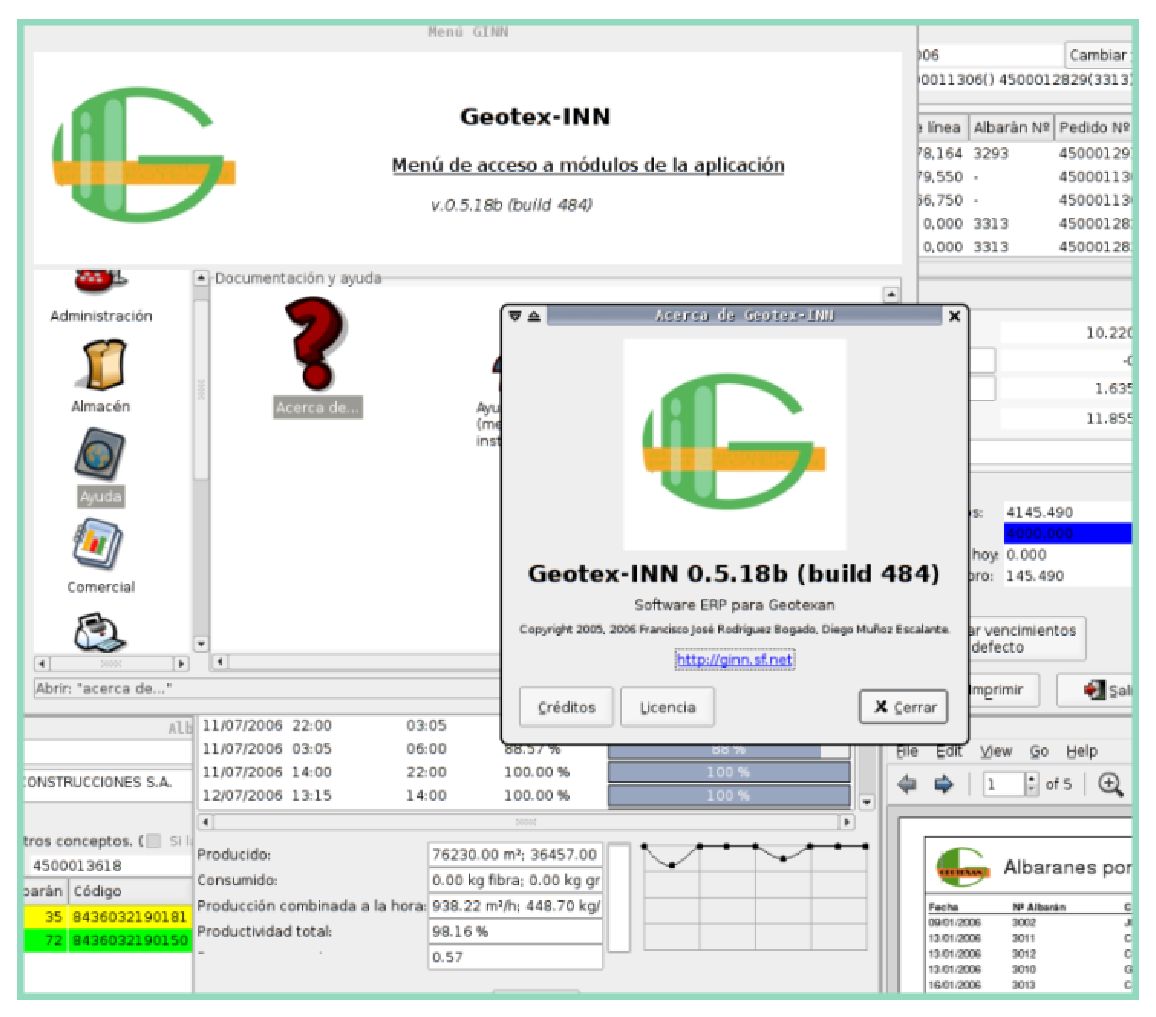
\includegraphics[width=12.5cm,height=10.5cm]{pantallazo.eps}\\
%                \else
%                    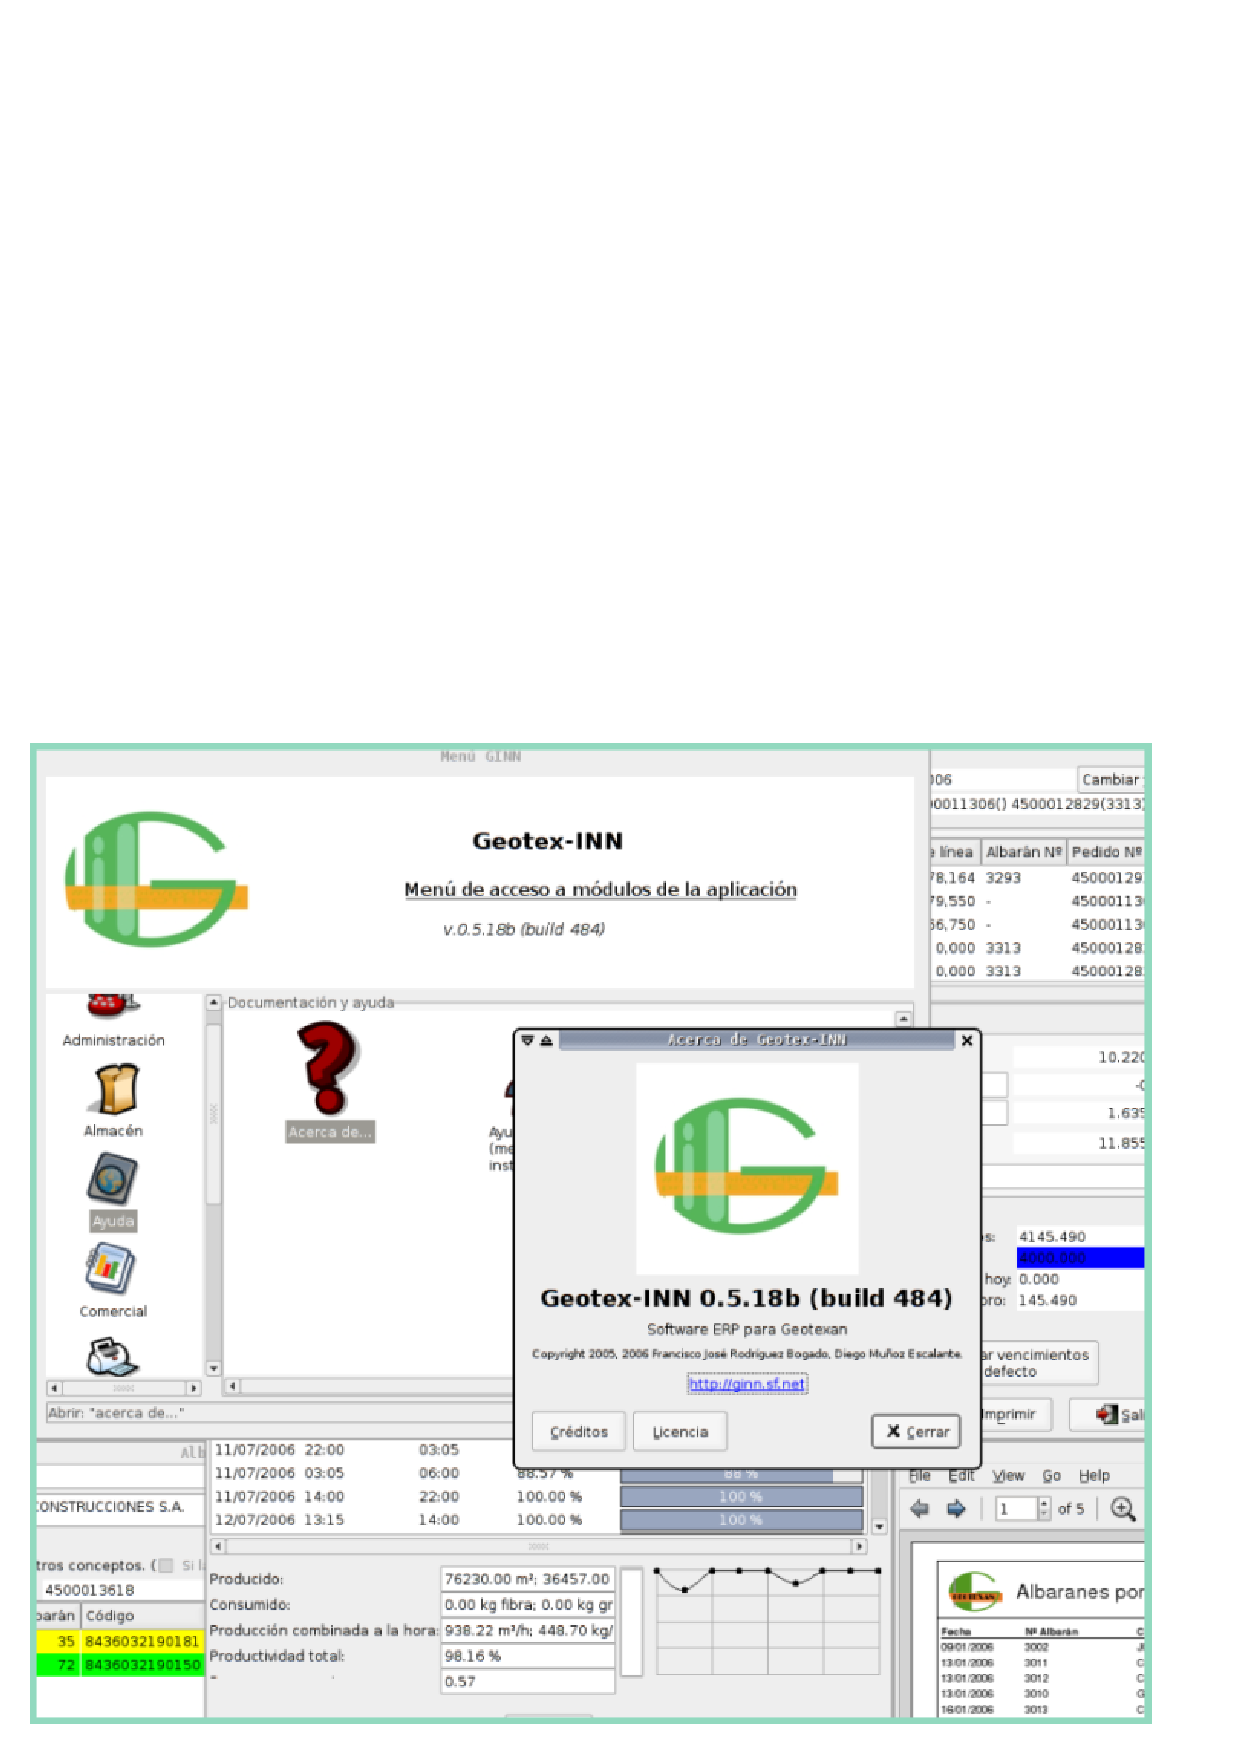
\includegraphics[width=12.5cm,height=10.5cm]{pantallazo.pdf}\\
%                \fi
                \caption{Captura de pantalla de la aplicación cliente.}
                \label{screenshot}
        \end{figure}\par
        \subsection{SLOC - COCOMO}
        \begin{verbatim}
Creating filelist for BD
Have a non-directory at the top, so creating directory top_dir
Adding /home/geotexan/geotexan/geotexinn02/./ChangeLog to top_dir
Adding /home/geotexan/geotexan/geotexinn02/./ChangeLog.bak to top_dir
Adding /home/geotexan/geotexan/geotexinn02/./COPYING to top_dir
Creating filelist for CVS
Adding /home/geotexan/geotexan/geotexinn02/./cvschangelogbuilder_geotexinn02.cache to top_dir
Creating filelist for doc
Creating filelist for formularios
Creating filelist for framework
Creating filelist for gajim-0.9.1
Adding /home/geotexan/geotexan/geotexinn02/./GPL to top_dir
Adding /home/geotexan/geotexan/geotexinn02/./gpl.txt to top_dir
Creating filelist for imagenes
Creating filelist for informes
Creating filelist for libgmail-0.1.3.3
Adding /home/geotexan/geotexan/geotexinn02/./post_outage.py to top_dir
Creating filelist for PyChart-1.39
Adding /home/geotexan/geotexan/geotexinn02/./README to top_dir
Creating filelist for SQLObject
Creating filelist for utils
Categorizing files.
Finding a working MD5 command....
Found a working MD5 command.
Computing results.


SLOC	Directory	SLOC-by-Language (Sorted)
52208   formularios     python=52208
24513   gajim-0.9.1     python=22155,sh=1710,ansic=648
11399   informes        python=11399
8874    SQLObject       python=8874
7742    framework       python=7686,sh=56
7160    PyChart-1.39    python=7160
2322    doc             sh=2039,python=283
2117    BD              python=2088,sh=29
969     libgmail-0.1.3.3 python=969
577     utils           python=577
11      top_dir         python=11
0       CVS             (none)
0       imagenes        (none)


Totals grouped by language (dominant language first):
python:      113410 (96.20%)
sh:            3834 (3.25%)
ansic:          648 (0.55%)




Total Physical Source Lines of Code (SLOC)                = 117,892
Development Effort Estimate, Person-Years (Person-Months) = 27.56 (330.71)
 (Basic COCOMO model, Person-Months = 2.4 * (KSLOC**1.05))
Schedule Estimate, Years (Months)                         = 1.41 (16.90)
 (Basic COCOMO model, Months = 2.5 * (person-months**0.38))
Total Estimated Cost to Develop                           = $ 1,428,660
 (average salary = $21,600/year, overhead = 2.40).
SLOCCount, Copyright (C) 2001-2004 David A. Wheeler
SLOCCount is Open Source Software/Free Software, licensed under the GNU GPL.
SLOCCount comes with ABSOLUTELY NO WARRANTY, and you are welcome to
redistribute it under certain conditions as specified by the GNU GPL license;
see the documentation for details.
Please credit this data as "generated using David A. Wheeler's 'SLOCCount'.
        \end{verbatim}
        \begin{figure}[!ht]
            \centering
%                \ifx\pdfoutput\undefined
                    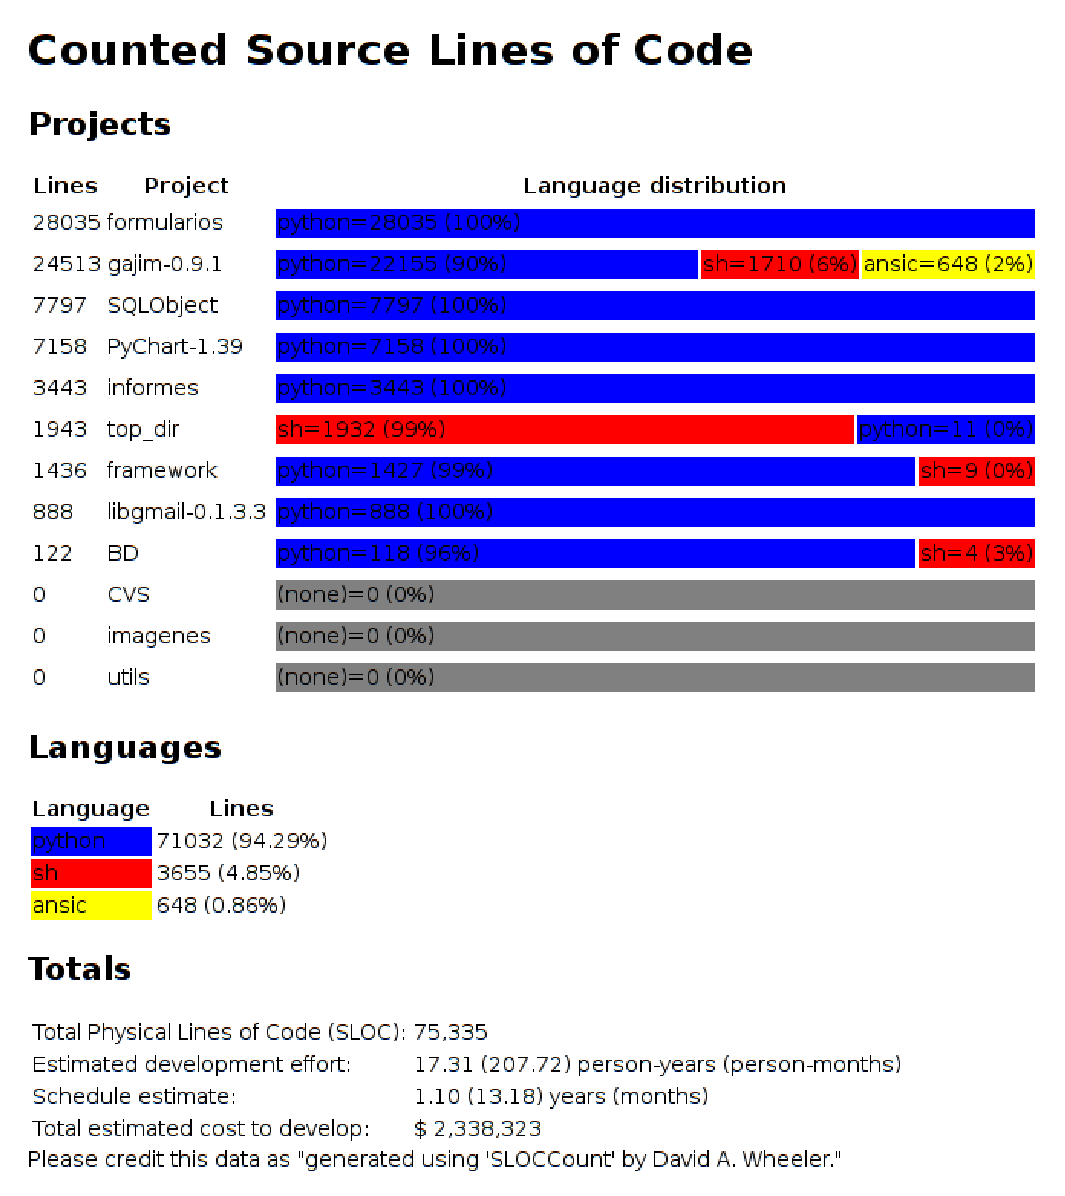
\includegraphics[width=12.5cm,height=13.5cm]{sloc.eps}\\
%                \else
%                    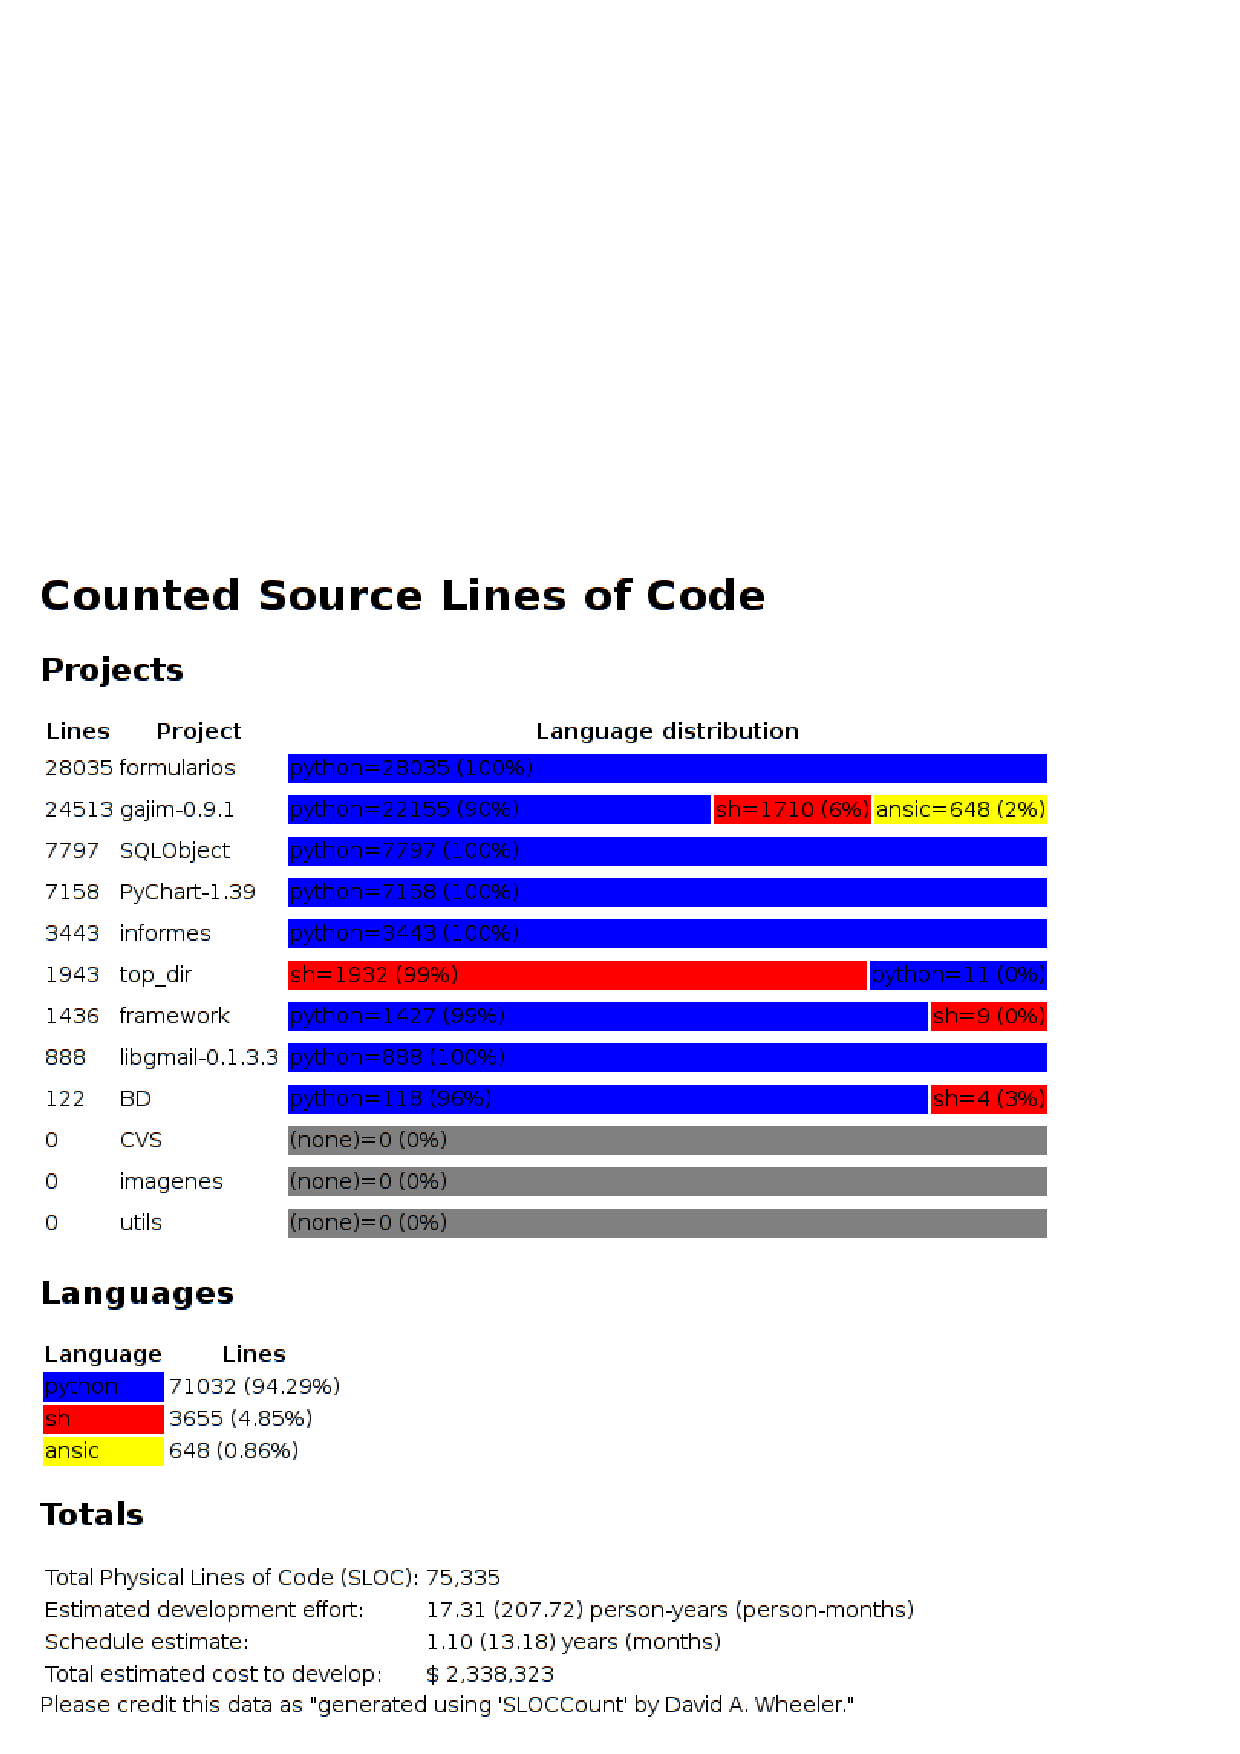
\includegraphics[width=12.5cm,height=13.5cm]{sloc.pdf}\\
%                \fi
                \caption{Source Lines Of Code y estimación COCOMO por SLOCCount.}
                \label{sloc}
        \end{figure}\par
        \subsection{CVS Changelog}
        \begin{figure}[!ht]
            \centering
%                \ifx\pdfoutput\undefined
                    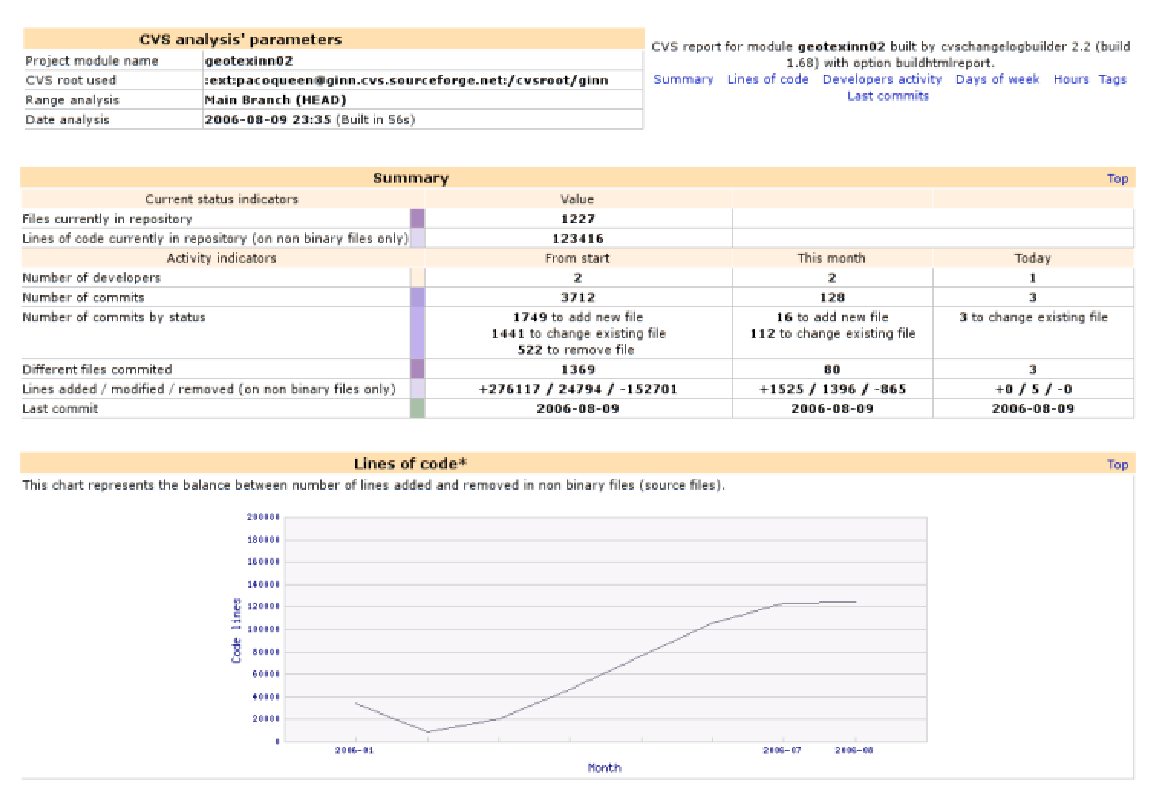
\includegraphics[width=12.5cm,height=9.3cm]{cvs0.eps}\\
%                \else
%                    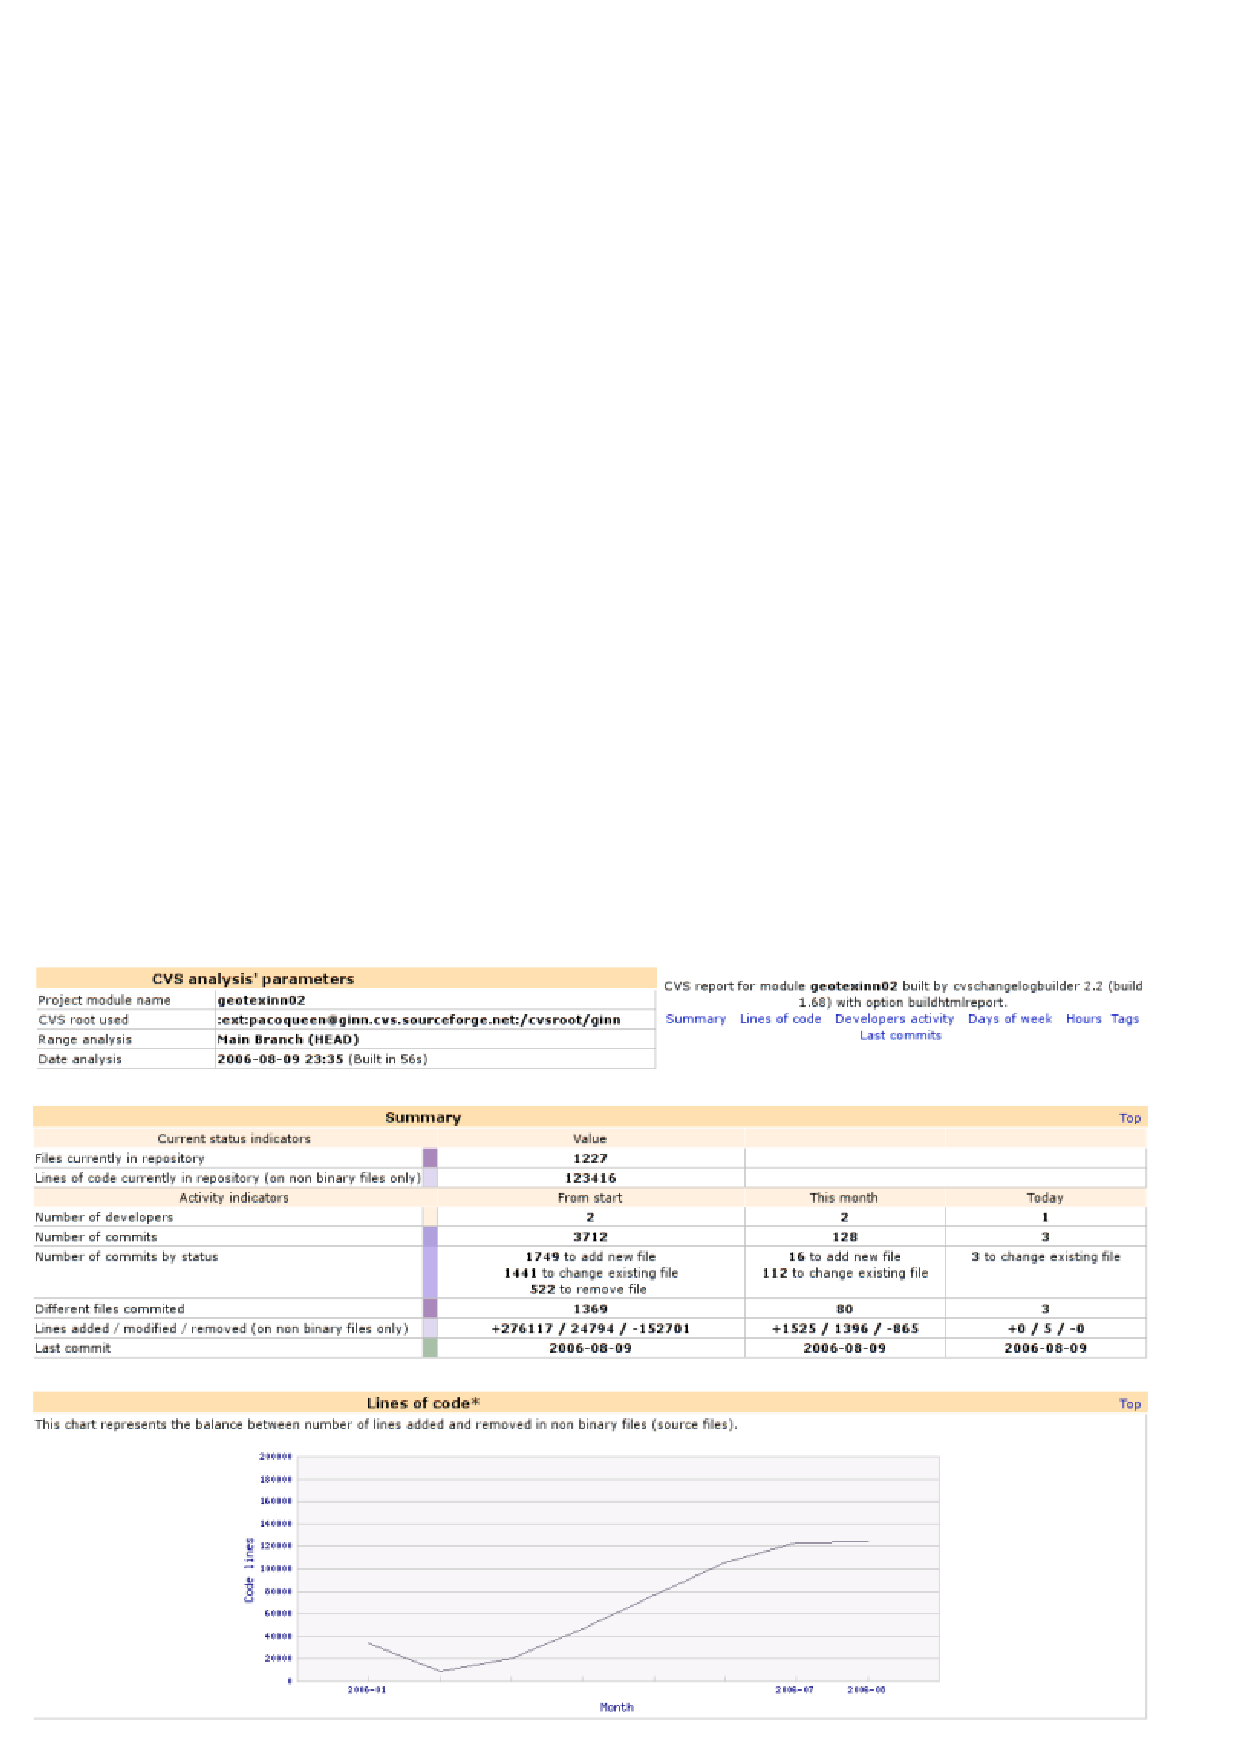
\includegraphics[width=12.5cm,height=9.3cm]{cvs0.pdf}\\
%                \fi
                \caption{Informe generado por \emph{cvschangelogbuilder 2.2}. -1/3-}
                \label{cvs0}
        \end{figure}\par
        \begin{figure}[!ht]
            \centering
%                \ifx\pdfoutput\undefined
                    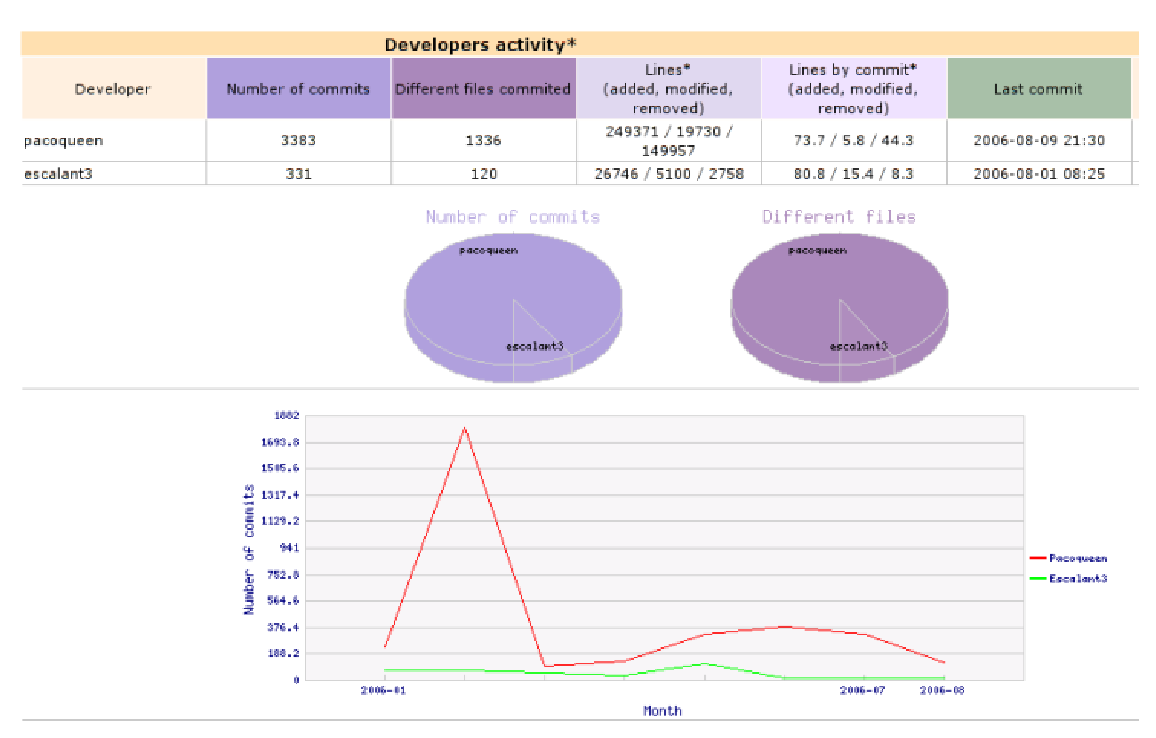
\includegraphics[width=12.5cm,height=9.3cm]{cvs1.eps}\\
%                \else
%                    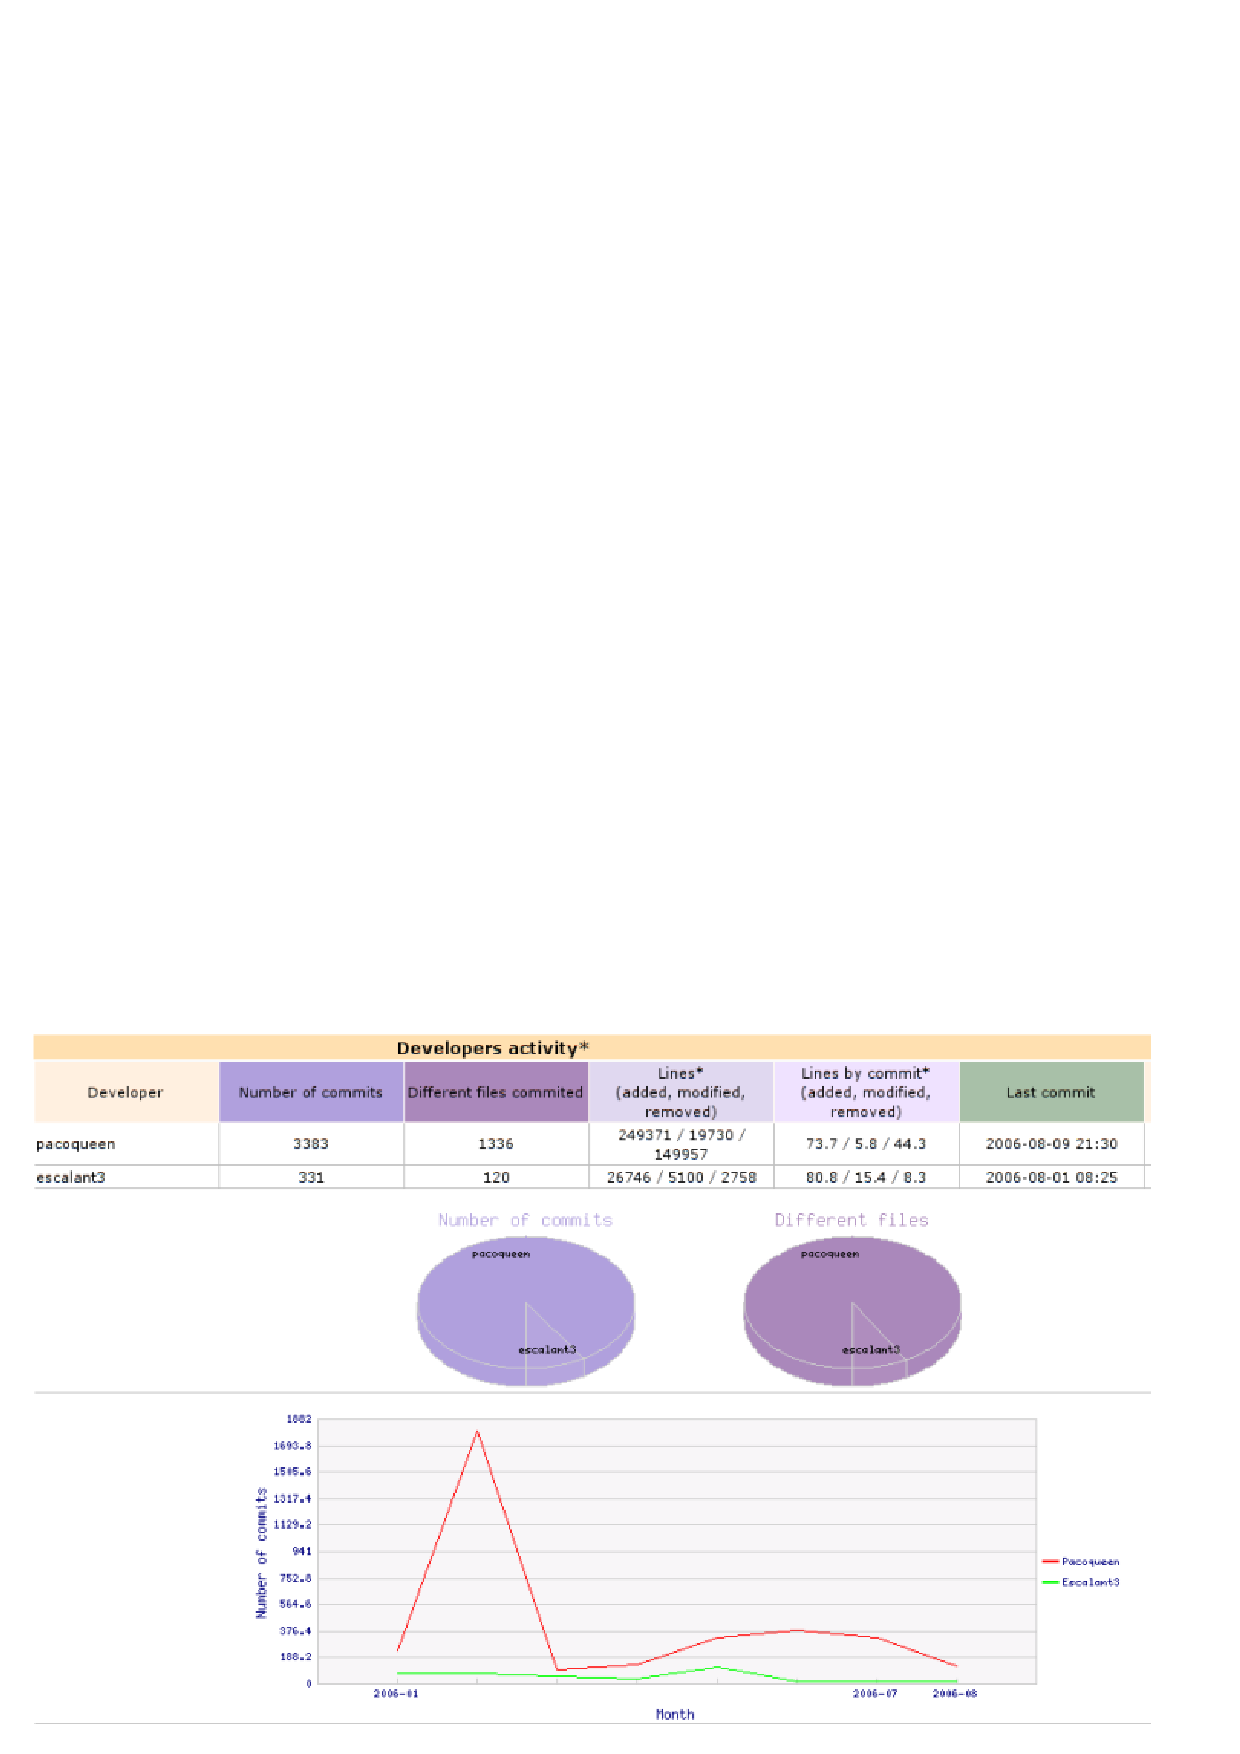
\includegraphics[width=12.5cm,height=9.3cm]{cvs1.pdf}\\
%                \fi
                \caption{Informe generado por \emph{cvschangelogbuilder 2.2}. -2/3-}
                \label{cvs1}
        \end{figure}\par
        \begin{figure}[!ht]
            \centering
%                \ifx\pdfoutput\undefined
                    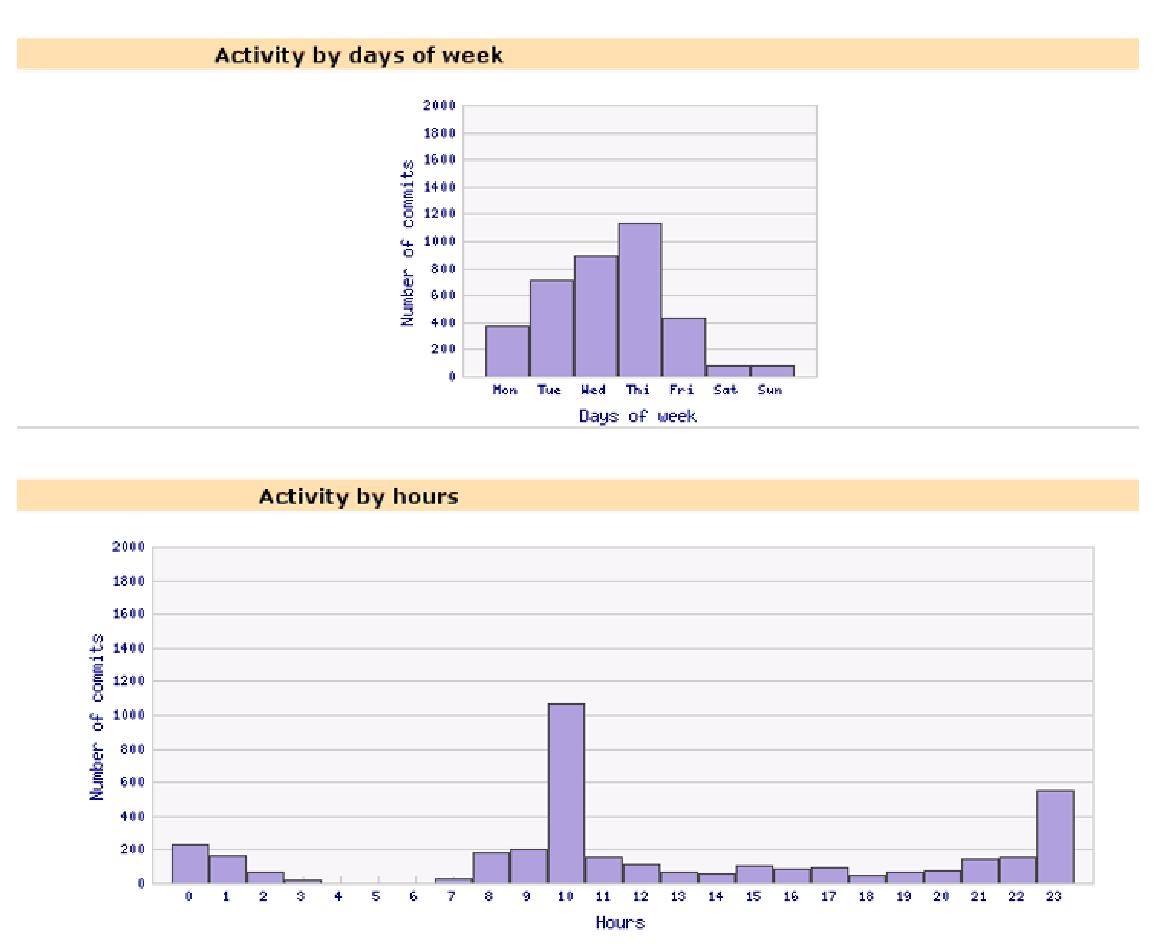
\includegraphics[width=12.5cm,height=9.3cm]{cvs2.eps}\\
%                \else
%                    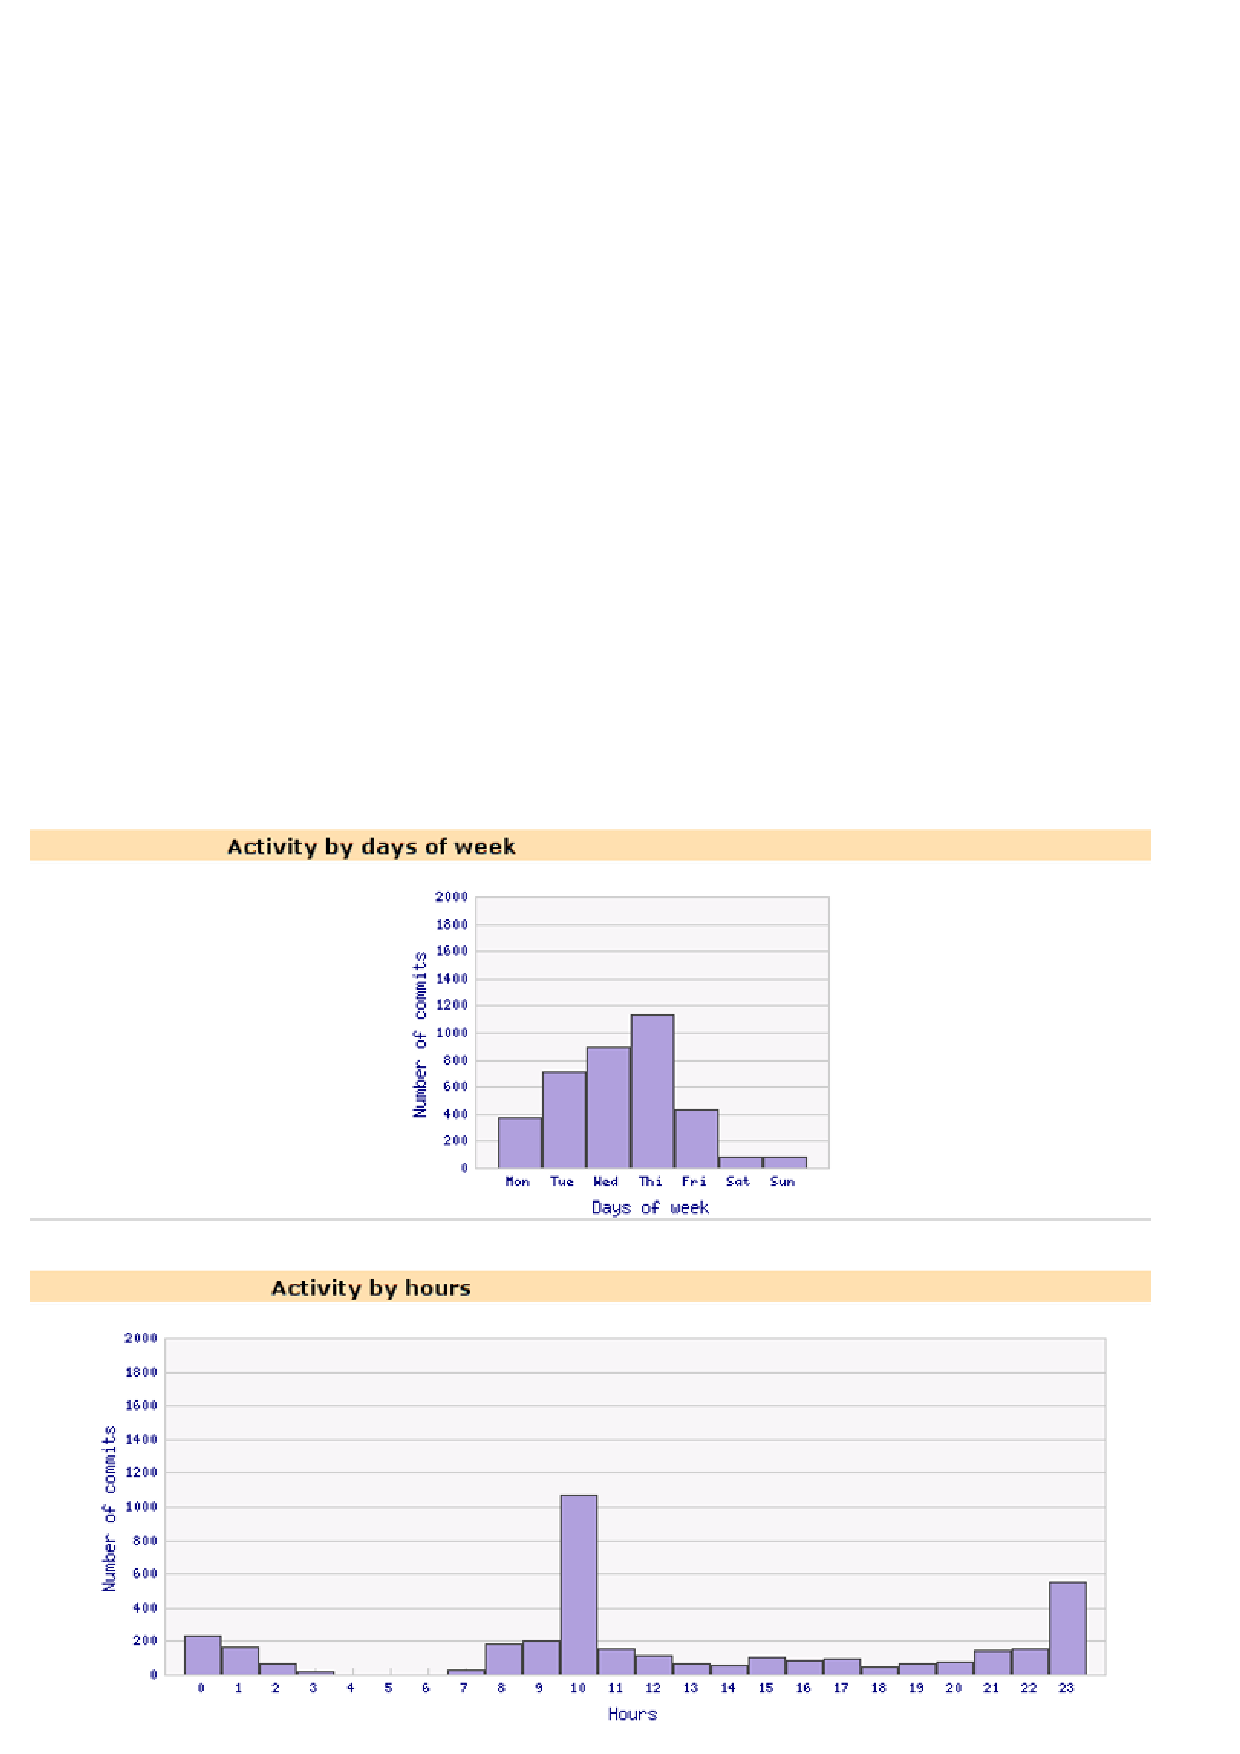
\includegraphics[width=12.5cm,height=9.3cm]{cvs2.pdf}\\
%                \fi
                \caption{Informe generado por \emph{cvschangelogbuilder 2.2}. -3/3-}
                \label{cvs2}
        \end{figure}\par
        \begin{figure}[!ht]
            \centering
%                \ifx\pdfoutput\undefined
                    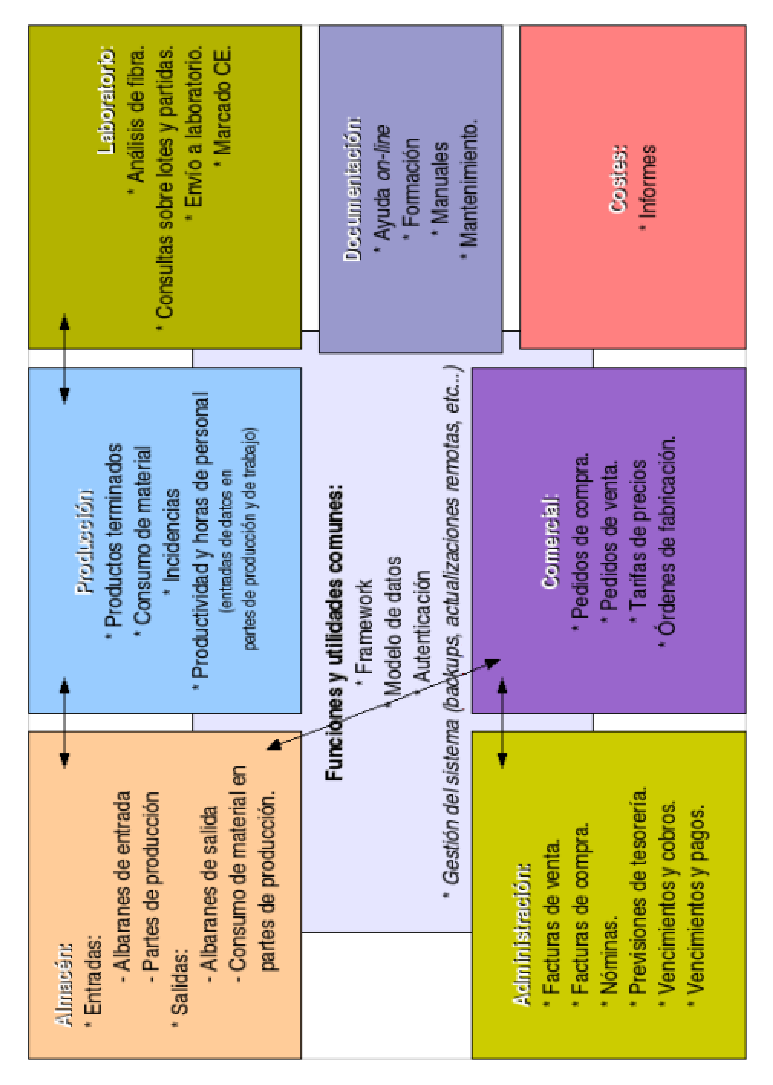
\includegraphics[width=12.5cm,height=18.8cm]{modulos.eps}\\
%                \else
%                    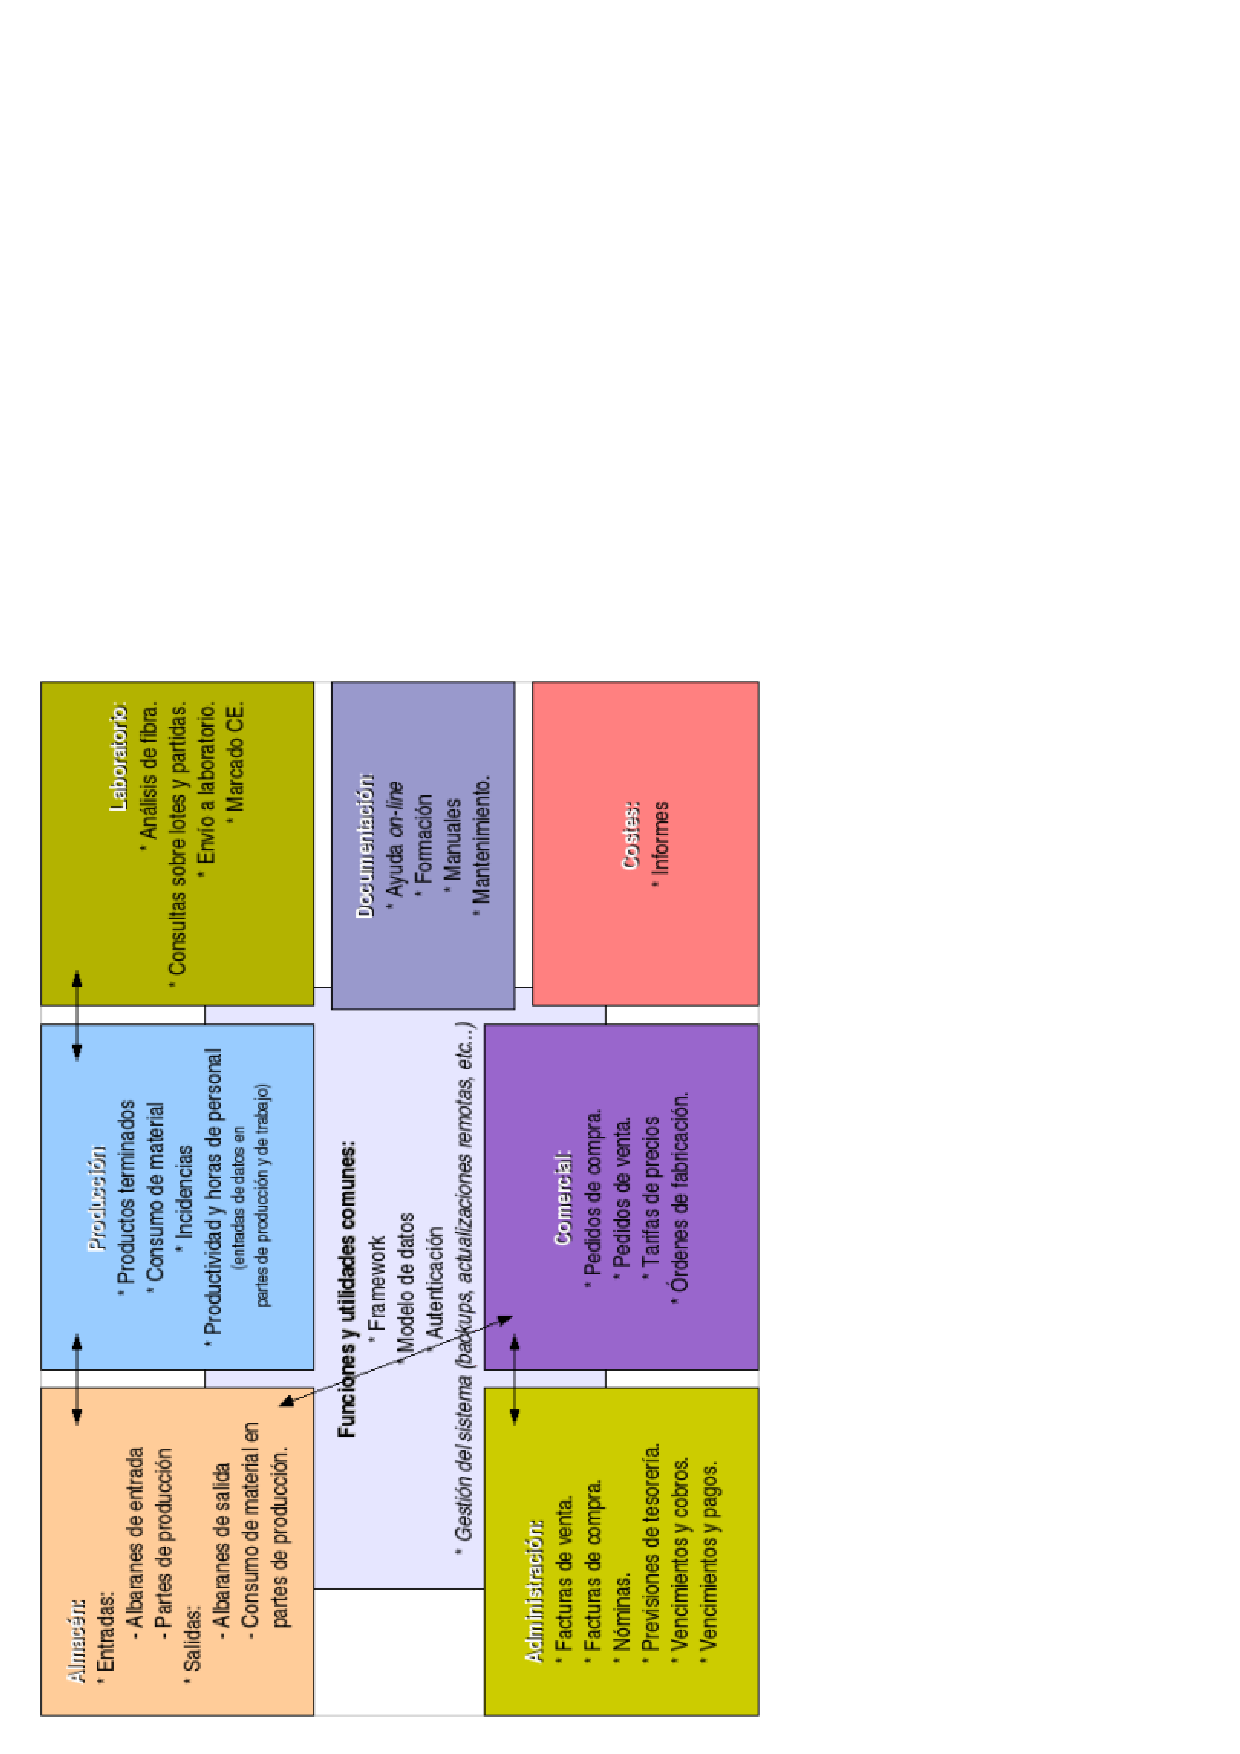
\includegraphics[width=12.5cm,height=18.8cm]{modulos.pdf}\\
%                \fi
                \caption{Esquema general de módulos.}
                \label{modulos}
        \end{figure}\par
        La implementación del ERP se conceptualizó como módulos interconectados con independencia funcional y mínimo acoplamiento, de manera que la cohesión entre ellos se ha ido afianzando a medida que se ha ido congelando el modelo de datos. Actualmente, los módulos de \textbf{Almac'en}, \textbf{Producción} y \textbf{Laboratorio} dependen entre sí al compartir datos y requisitos funcionales --recogidos en el documento de requisitos--. Por ejemplo, para que un material salga del almac'en es necesario que por un lado se haya producido y cuente con un código unívoco de trazabilidad; y por otro, que en el análisis de calidad del laboratorio haya superado ciertos baremos (marcado C\euro). Cumplidos estos dos requisitos, la salida se hace efectiva mediante un albarán de salida.\\
        Cada uno de los ítems mostrados en la figura \ref{modulos} están cubiertos por al menos una ventana de la \emph{GUI} dentro del directorio \texttt{formularios}. El uso de una u otra clase derivada de la clase padre \texttt{ventana.py} --en caso de que haya más de una y no cuenten con permisos granulares lectura, escritura y modificación\footnote{Como por ejemplo los partes de producción, a diferencia de la mayoría de las ventanas donde los permisos son únicamente de acceso/ejecución. Para más información v'ease la gestión de permisos, que está suficientemente documentada en \texttt{menu.py}, \texttt{autenticacion.py} y la tabla \texttt{permisos} de \texttt{tablas.sql}}-- para manipular el alta, baja, modificación y consulta de objetos depende del tipo de usuario que tendrá acceso a ella.
        De manera similar, el módulo de \textbf{Almac'en} se encuentra relacionado con el \textbf{Comercial}, y 'este con el de \textbf{Administración}. Cualquier cambio en alguno de ellos afectaría al resto, por lo que es necesario un análisis de impacto ante cualquier cambio. Para la gestión de configuraciones se puede consultar el documento de requisitos actualizado (versión 3.0, en la fecha de este memorándum) en conjunto con la documentación de las clases afectadas, tanto en el catálogo de objetos persistentes (\texttt{pclases}) como en las ventanas de la \emph{GUI} dentro del directorio \texttt{formularios} e informes \texttt{informes y geninformes.py} \ref{sec:doc} que dependan y recojan las funcionalidades y datos a modificar. Si el cambio afecta al modelo de datos es altamente recomendable preservar la compatibilidad hacia atrás con las copias de seguridad existentes. En otro caso, el procedimiento debería ser:
        \begin{enumerate}
        \item Modificar el \emph{script} \texttt{tablas.sql} para recoger la nueva información y relaciones.
        \item Asegurar semántica y al menos la 3FN\footnote{Tercera forma normal} del modelo entidad-relación.
        \item Verificar que el dominio de los campos está soportado por el ORM\footnote{Object Relational Mapper} SQLObject.
        \item Levantar \textbf{una nueva base de datos} con el nuevo modelo de datos.
        \item Modificar \texttt{pclases.py} de acuerdo al nuevo \texttt{tablas.sql}.
        \item Mover las tuplas de la base de datos antigua a la nueva \textbf{a trav'es de objetos de pclases}. De esta manera es más sencilla hacer la traslación de campos obsoletos al nuevo dominio de datos, usar valores por defecto, conservar las relaciones entre claves ajenas, etc.
        \item Realizar una nueva copia de seguridad de los datos convertidos.
        \item Detener y eliminar la base de datos antigua.
        \item Renombrar y restaurar (\texttt{create\_and\_populate.sh}) la copia de seguridad, ahorrándonos el cambio de configuración en el archivo \texttt{.conf}.
        \end{enumerate}
    \section{Planificación}
    \begin{figure}[!ht]
        \centering
%            \ifx\pdfoutput\undefined
                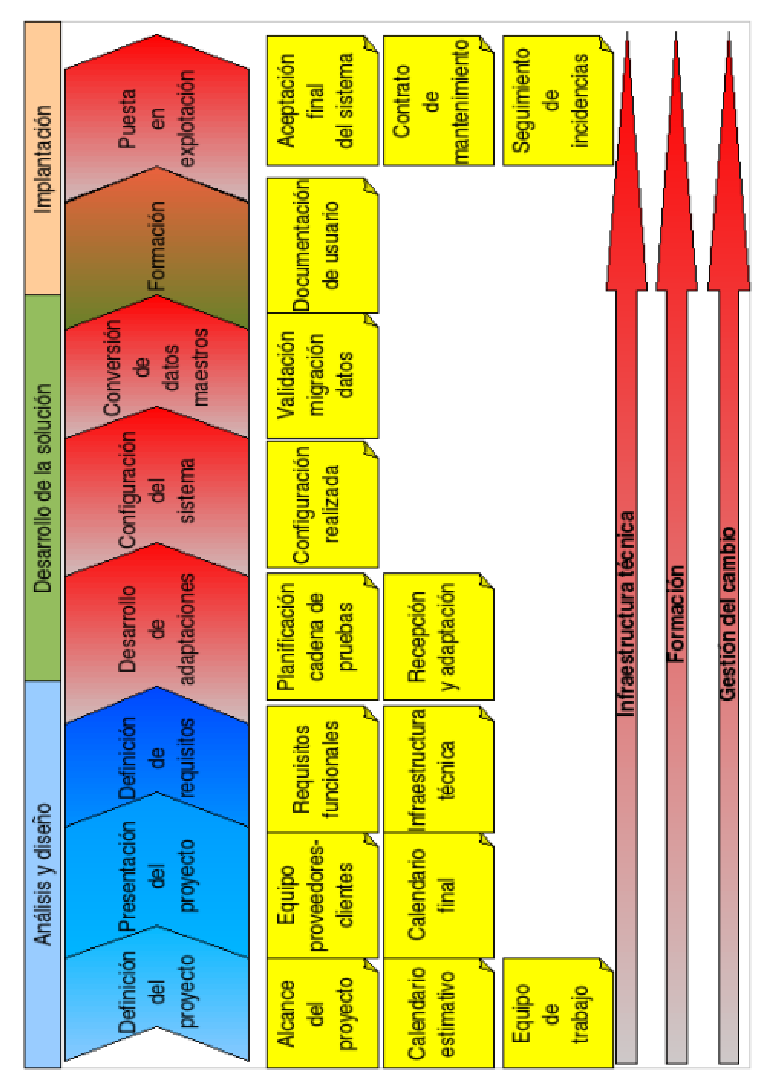
\includegraphics[width=12.5cm,height=18.9cm]{implantacion.eps}\\
%            \else
%                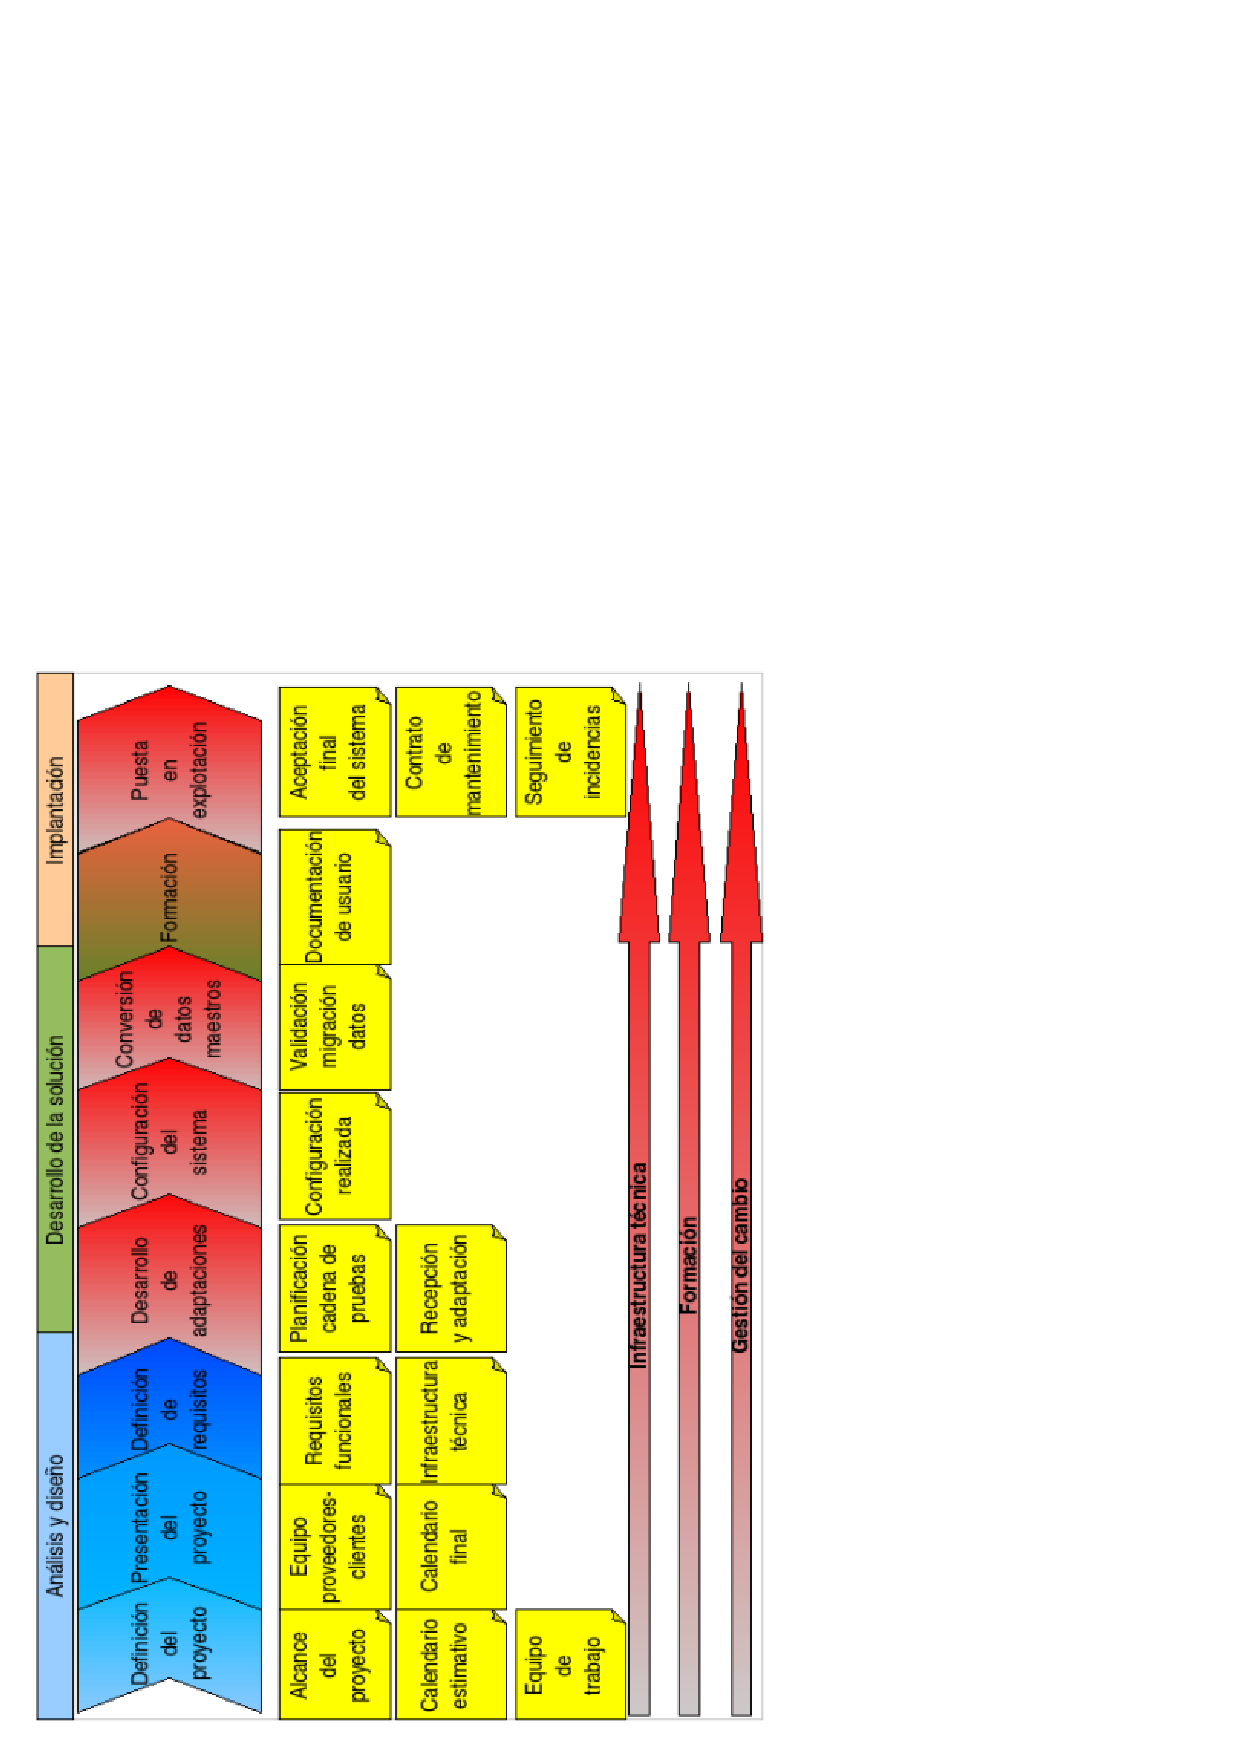
\includegraphics[width=12.5cm,height=18.9cm]{implantacion.pdf}\\
%            \fi
            \caption{Costes de implantación en un proyecto de ingeniería del software.}
            \label{implantacion}
    \end{figure}\par
    Calendario del \textbf{proyecto desarrollo \emph{software}}\footnote{Cotejado con la planifiación inicial prevista (recogida en el documento de requisitos) y la real (recogida en el \emph{Changelog}}:
        \begin{center}
            \begin{longtable}{|| c | l | p{0.7\textwidth} ||}
                \hline
                \hline
                \emph{\textbf{Fecha}} & \emph{\textbf{Fase}} & \emph{\textbf{Comentarios}}\\
                \hline
                \hline
                \textbf{02/06/05} & Análisis & Aceptación del presupuesto. \\
                \hline
                15/06/05 & Análisis & Documento de requisitos (ver. 1). \\
                \hline
                16/06/05 & Análisis & Retraso en reunión de revisión de requisitos. \\
                \hline
                \textbf{30/06/05} & Análisis & Reunión de revisión de requisitos. \\
                \hline 
                01/07/05 & Análisis & Corrección de requisitos de usuario. \\
                \hline 
                \textbf{05/07/05} & Análisis & Corrección PDS v2 y formalización del documento de requisitos (versión 3). \\
                \hline
                \hline
                06/07/05 & Diseño & Análisis de requisitos funcionales y no funcionales. \\
                \hline
                08/07/05 & Diseño & Análisis de requisitos de información. \\
                \hline 
                11/07/05 & Diseño & Generación de prototipos. \\
                \hline
                12/07/05 & Diseño & Planificación temporal. \\
                \hline
                \hline
                13/07/05 & Codificación & Ingeniería de arquitectura. \\
                \hline
                17/08/05 & Codificación & Desarrollo de funciones gen'ericas. \\
                \hline
                12/09/05 & Codificación & Módulo de gestión de almac'en. \\
                \hline
                04/10/05 & Codificación & Módulo de administración. \\
                \hline
                \textbf{10/10/05} & Codificación & Instalación hardware. \\
                \hline
                \textbf{16/10/05} & Codificación & Instalación arquitectura. \\
                \hline
                24/10/05 & Codificación & Módulo de gestión comercial. \\
                \hline
                03/11/05 & Codificación & Módulo de producción. \\
                \hline
                \textbf{16/11/05} & Codificación & Actualización plataforma de explotación. \emph{Bugtracker} y \emph{wiki} en \emph{Sourceforge}.\\
                \hline
                17/11/05 & Codificación & Módulo de costes e informes. \\
                \hline
                \textbf{30/11/05} & Codificación & Actualización plataforma de explotación. \\
                \hline
                05/12/05 & Codificación & Módulo de laboratorio. \\
                \hline
                \textbf{14/12/05} & Codificación & Actualización plataforma de explotación. Importación de datos existentes. \\
                \hline
                \textbf{20/12/05} & Codificación & Actualización plataforma de explotación. Intrucción datos adicionales. \\
                \hline
                \textbf{11/01/06} & Pruebas & Reunión validación. Inicio versión 0.2b. \\
                \hline
                \textbf{17/01/06} & Pruebas & Pruebas funcionales y unitarias. \\
                \hline
                \textbf{19/01/06} & Análisis & Análisis de nuevos requisitos y modificación de existentes. \\
                \hline
                \textbf{24/01/06} & Codificación & Iteración de versión --revisión--. \\
                \hline
                \textbf{30/01/06} & Codificación & Análisis de nuevos requisitos, modificación de existentes y nueva planificación temporal. \\
                \hline
                \textbf{07/02/06} & Codificación & Iteración de versión --revisión--. \\
                \hline
                \hline
                \textbf{13/02/06} & Codificación & Modificaciones no previstas en partes de producción (balas B, cambios funcionales en partes de balas, listado de rollos en almacén, series numéricas independientes de facturas en clientes\dots) \\
                \hline
                \textbf{16/02/06} & Codificación & Ajustes partes, tarifas, etc. \\
                \hline
                \textbf{02/03/06} & Codificación & Modificaciones en facturas, productividad en partes, estudio abonos\dots\\
                \hline
                \textbf{16/03/06} & Codificación & Implantación gestión de abonos, modificaciones en consulta de productividad, etc. \\
                \hline
                \textbf{04/04/06} & Codificación & Formación becario, recogida de partes de producción, verificación impresión de facturas\dots \\
                \hline
                \textbf{02/05/06} & Codificación & Implantación y formación laboratorio, instalación de informes y gestión de usuarios. \\
                \hline
                \textbf{09/05/06} & Codificación & Reunión de validación y planificación temporal. Cambio de versión mayor. \\
                \hline
                \textbf{10/05/06} & Codificación & Instalación y formación planta. Nuevos requisitos y ampliaciones. \\
                \hline
                \textbf{16/05/06} & Codificación & Validación y formación planta y encargado almac'en. Instalación de modificaciones recogidas el 10/05/06. \\
                \hline
                \textbf{18/05/06} & Codificación & Validación y formación director comercial. \\
                \hline
                \textbf{19/05/06} & Codificación & Validación y formación laboratorio. \\
                \hline
                \textbf{23/05/06} & Codificación & Validación y formación ofic. admisitración (J). Recogida requisitos módulo de nóminas. \\
                \hline
                \textbf{25/05/06} & Codificación & Validación y formación ofic. administración (M). Recodiga requisitos pagarés de pagos. Modificación pagarés de cobros, facturas de venta\dots \\
                \hline
                \textbf{30/05/06} & Codificación & Instalación previsiones de cobro. Formación jefes de línea y de turno. Nuevos requisitos partes de producción. \\
                \hline
                \textbf{05/06/06} & Codificación & Instalación en equipo director t'ecnico. Instalación y formación de plásticos en partes de producción, formulación y descuentos automáticos\dots \\
                \hline
                \textbf{01/08/06} & Codificación & Implantación cobros, pagar'es, nóminas, calendarios laborales, configuración etiquetadora de códigos de barras línea de geotextiles\dots \\
                \hline
                \hline
            \end{longtable}
        \end{center}
    \section{Diagramas}
    El diagrama de clases completo, al igual que el entidad-relación del modelo de datos, se encuentran reducidos dado el gran tamaño de los mismos\footnote{El diagrama de clases actual --provisional--, por ejemplo, tiene un tamaño de 26.667 x 1.095 píxeles}. El diagrama entidad-relación se puede imprimir cómodamente en 2x8 A4. Ambos se pueden descargar a tamaño completo del \emph{wiki} del proyecto, así como un \emph{script} para dividirlos y poderlos imprimir más fácilmente:\\
\iconomargen{3}{link} \texttt{http://ginn.sourceforge.net/wiki/DBDesign2}.\\
    Información adicional respecto a algunos de estos diagramas se puede encontrar en: 
    \begin{itemize}
        \item \texttt{http://ginn.sourceforge.net/wiki/EsquemaModulos}
        \item \texttt{http://ginn.sourceforge.net/ginn.html}
    \end{itemize}
    Otros diagramas UML se irán agregando a este documento y a la web conforme se vayan completando al congelar las funcionalidades (\texttt{v1.0rc}) una vez est'en todas las incidencias y nuevos requisitos y casos de uso resueltos.
    \begin{figure}[!ht]
        \centering
%            \ifx\pdfoutput\undefined
                
\includegraphics[width=14.5cm]{ginn_pclases.eps}\\
%            \else
%                
\includegraphics[width=14.5cm]{ginn_pclases.pdf}\\
%            \fi
            \caption{\emph{Thumbnail} del diagrama de clases.}
            \label{diagrama:clases}
    \end{figure}\par

    \begin{figure}[!ht]
        \centering
%            \ifx\pdfoutput\undefined
                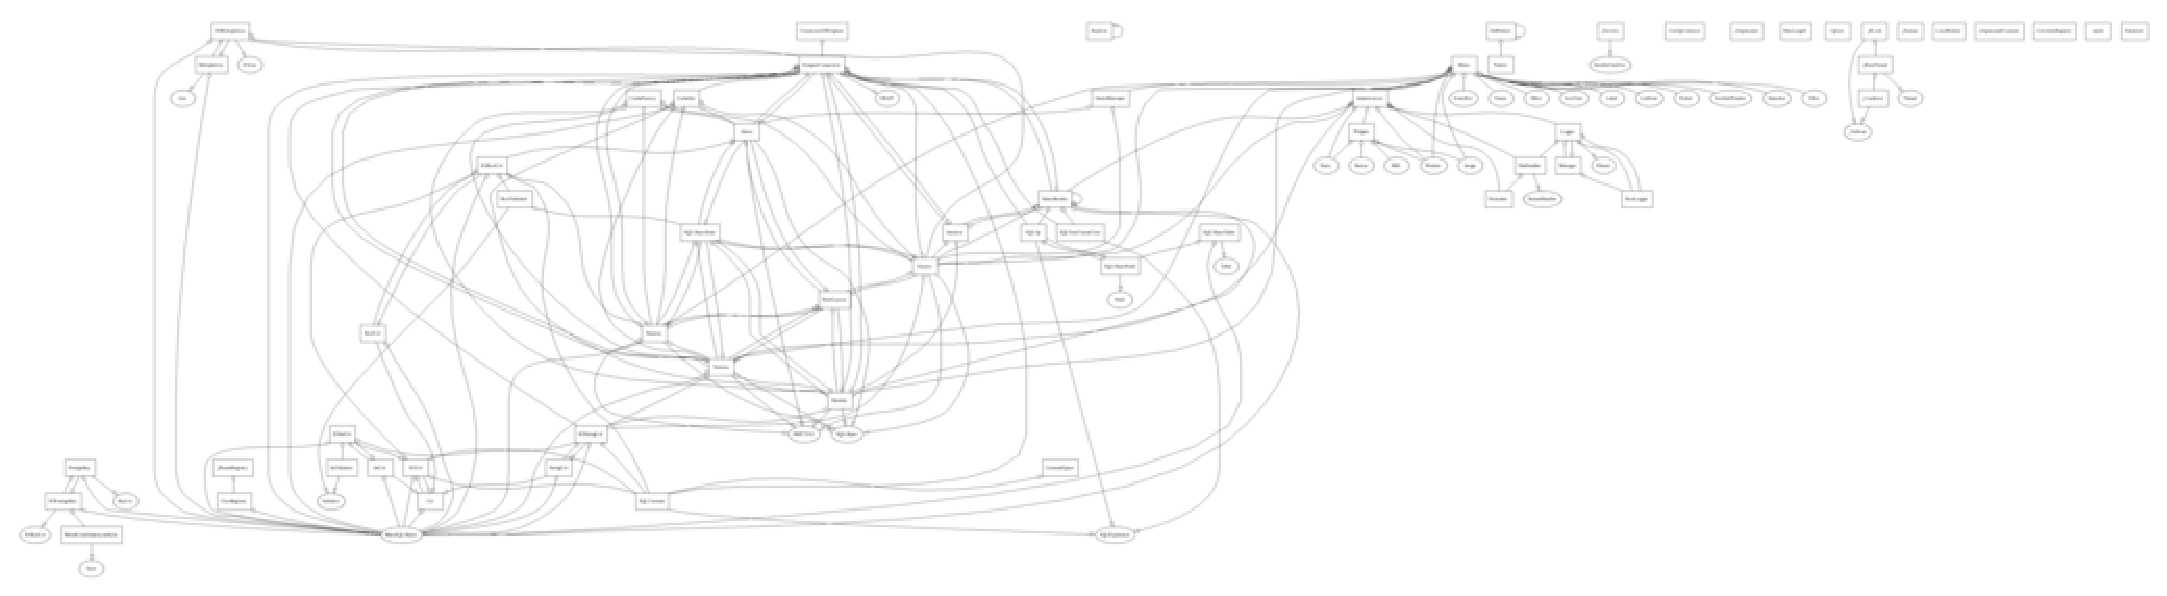
\includegraphics[width=14.5cm]{ginn_clases.eps}\\
%            \else
%                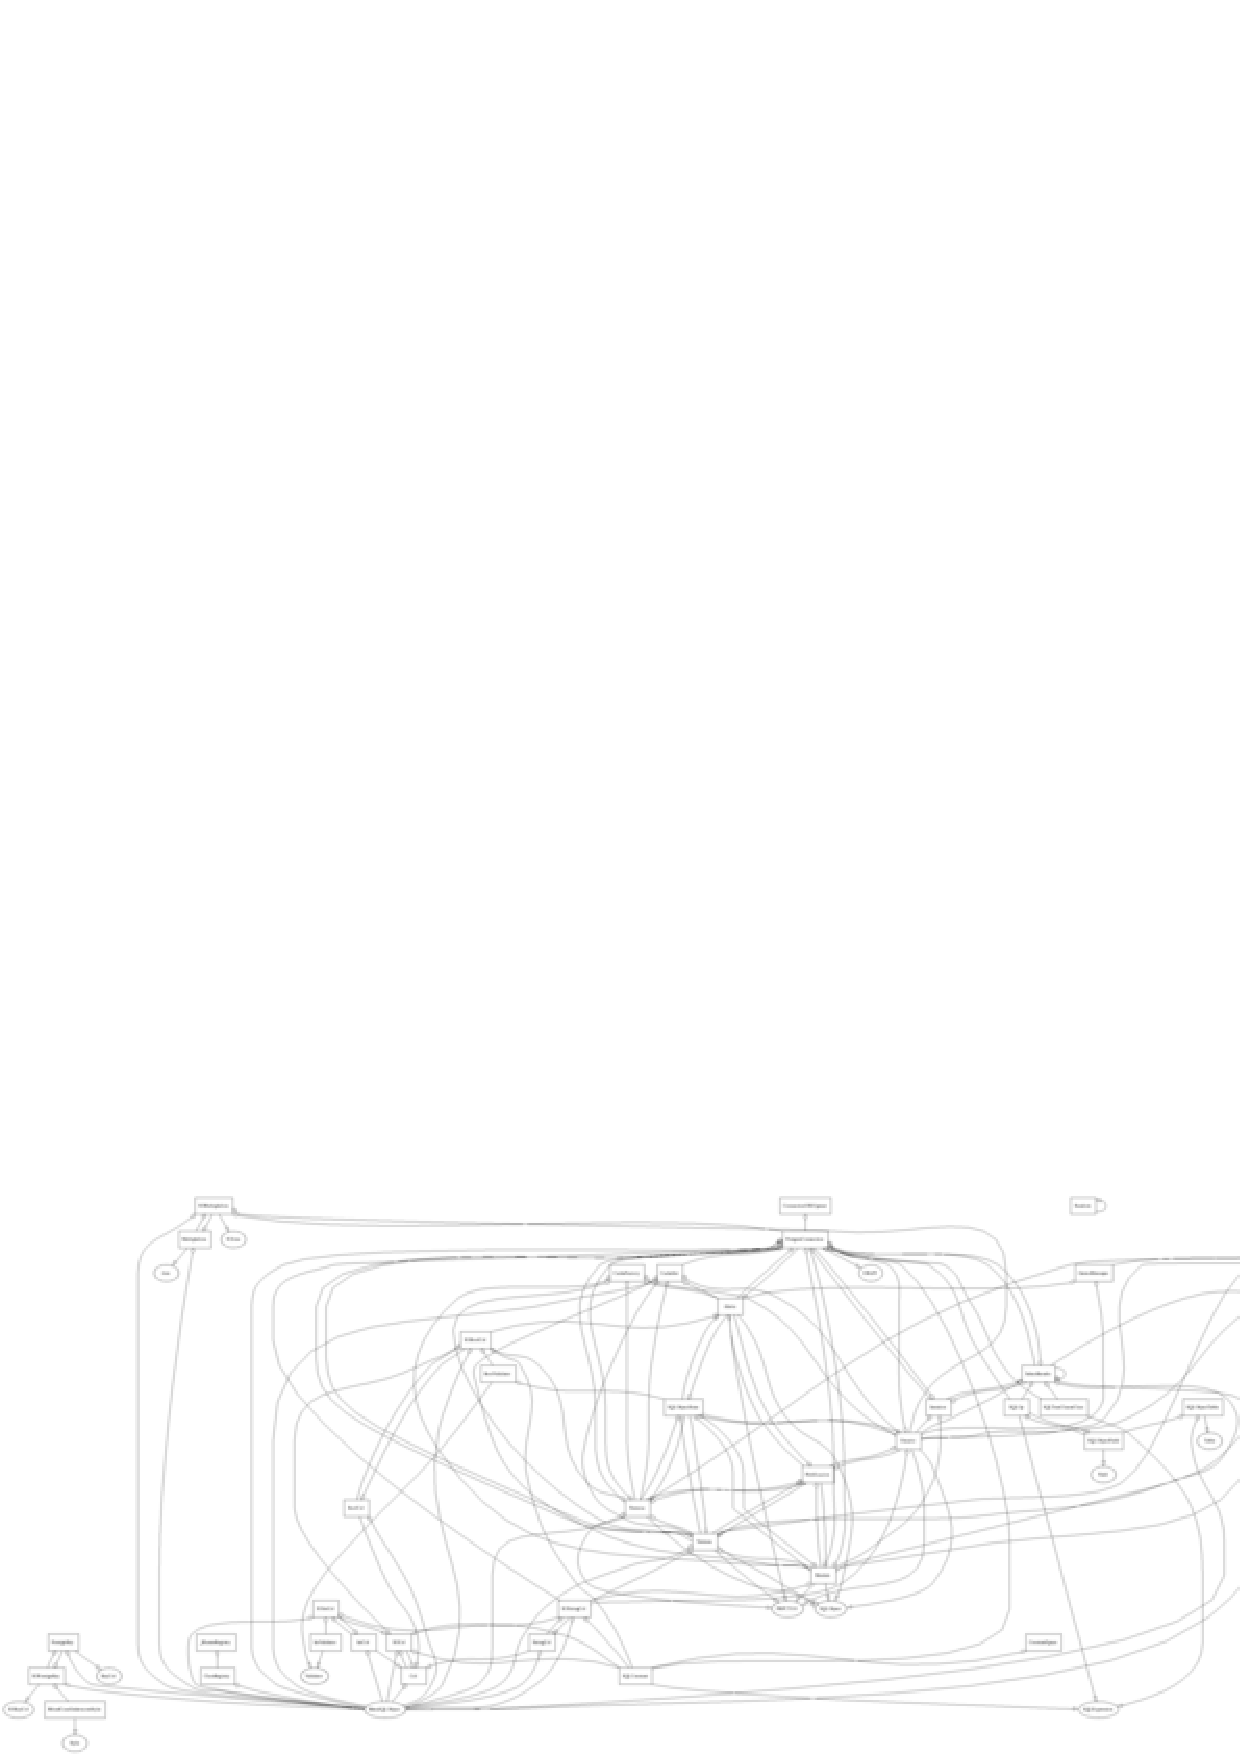
\includegraphics[width=14.5cm]{ginn_clases.pdf}\\
%            \fi
            \caption{Diagrama de ejecución.}
            \label{diagrama:ejecucion}
    \end{figure}\par
    
    \begin{figure}[!ht]
        \centering
%            \ifx\pdfoutput\undefined
                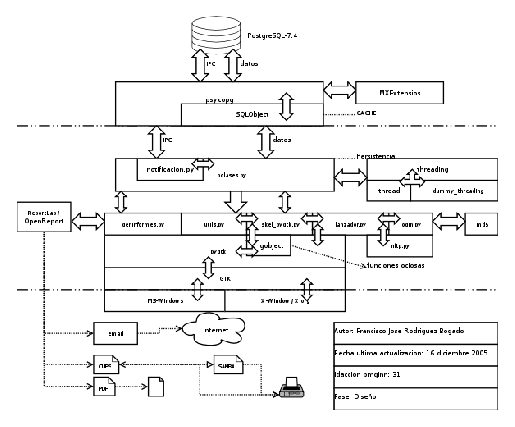
\includegraphics[width=10cm]{Esquema_modulos.eps}\\
%            \else
%                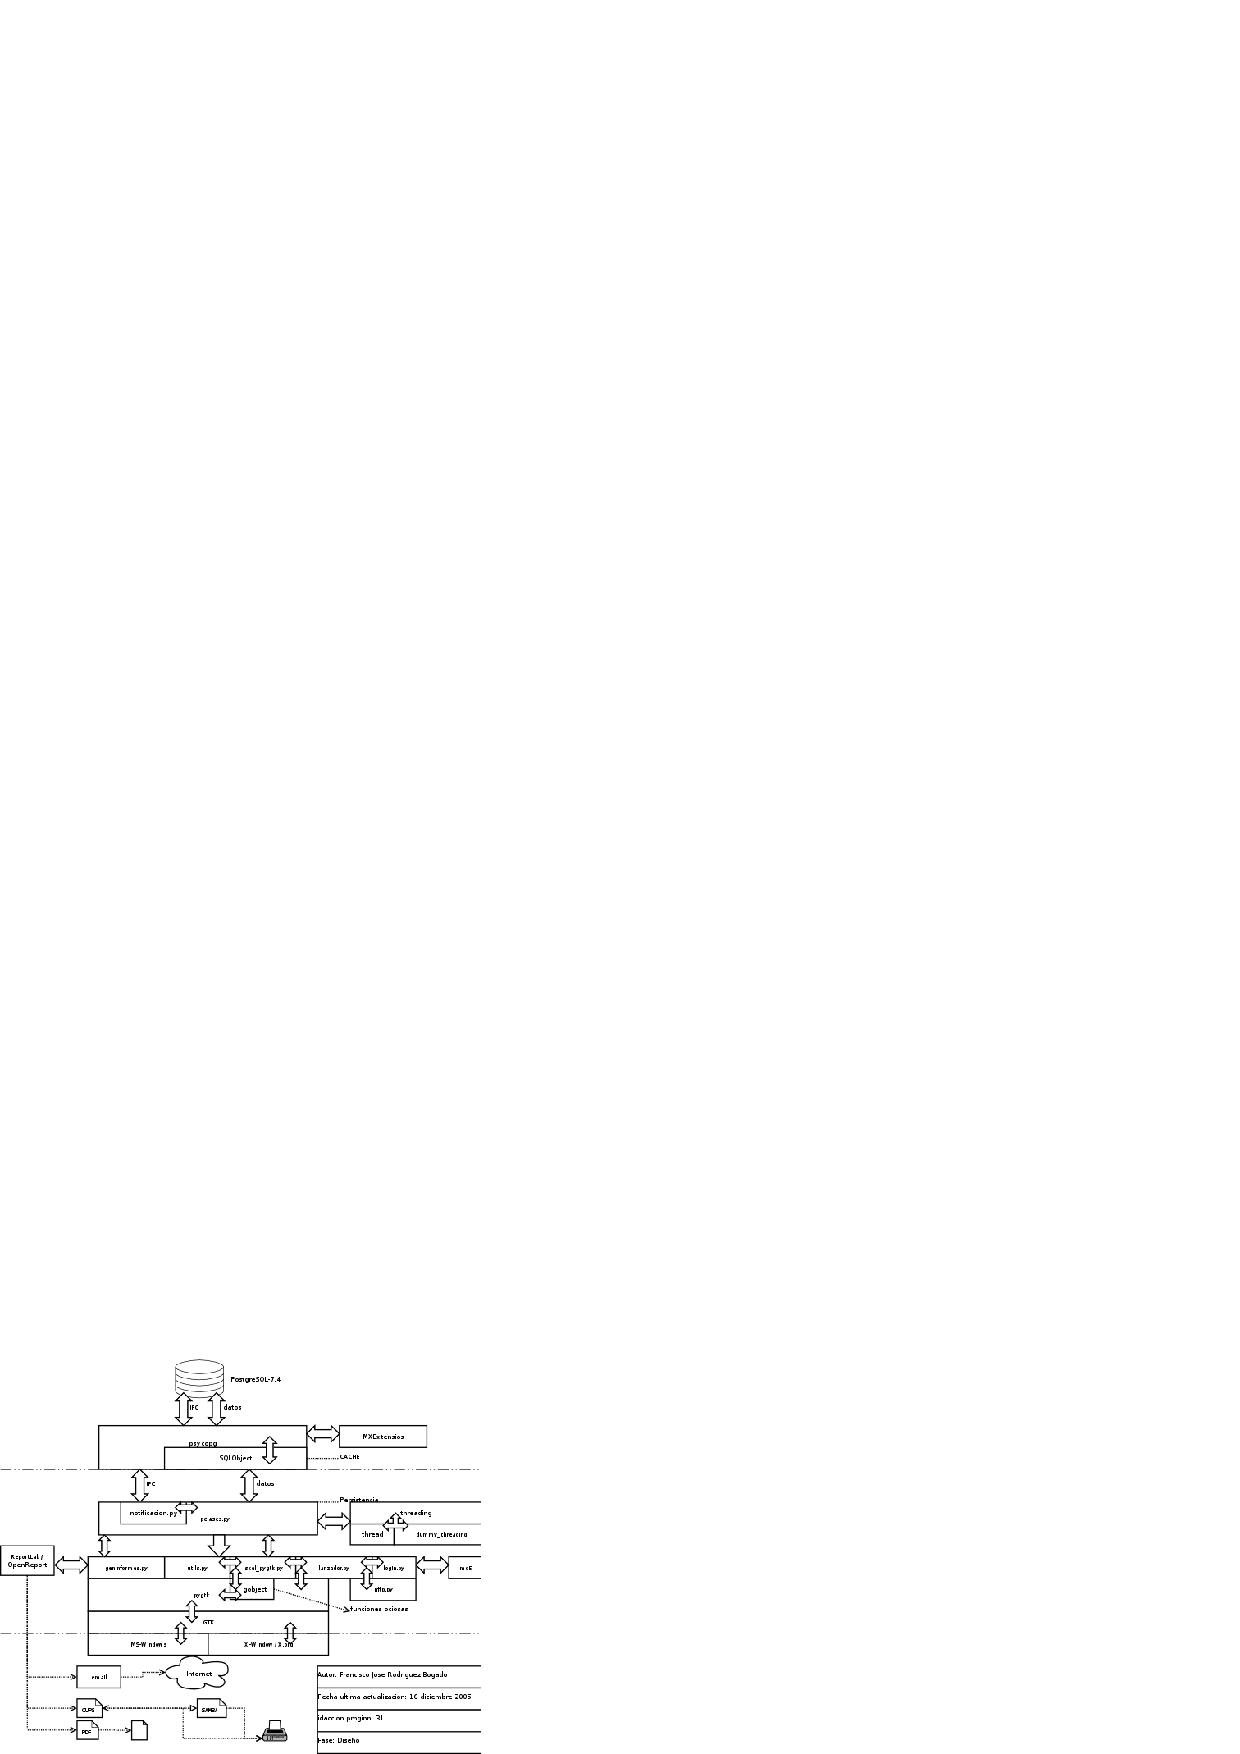
\includegraphics[width=10cm]{Esquema_modulos.pdf}\\
%            \fi
            \caption{Diagrama de componentes: Interacción de los módulos principales.}
            \label{diagrama:componentes}
    \end{figure}\par

    \begin{figure}[!ht]
        \centering
%            \ifx\pdfoutput\undefined
                \includegraphics[height=21.5cm]{ginn.eps}\\
%            \else
%                \includegraphics[height=21.5cm]{ginn.pdf}\\
%            \fi
            \caption{Diagrama entidad-relación de la base de datos.}
            \label{diagrama:er}
    \end{figure}\par
    
    \section{\emph{Roadmap} y estadísticas}
        \begin{center}
            \begin{tabular}{|| l | l ||}
            \hline
            \hline
            \multicolumn{2}{c}{\textbf{Control de versiones: Historial de versiones menores}} \tabularnewline
            % Control de versiones.
            % mayor.menor.release(alpha|beta|release candidate)
            \hline
            0.1b & Primera versión funcional. \\
            \hline
            0.2b & Reestructuración completa de casos de uso. \\
            \hline
            0.3b & Primera \emph{beta} funcional despu'es de los cambios de requisitos. \\
            \hline
            0.4b & Integración con módulo de \textbf{laboratorio}. \\
            \hline
            0.5b & Versión de integración con \textbf{\emph{LOGIC}}. \\
            \hline
            0.6b & Versión de integración con \textbf{nóminas}. \\
            \hline
            0.7b & Todos los módulos integrados. Fase de \textbf{pruebas}. \\
            \hline
            \hline
            0.8b & Resolución de incidencias. \\
            \hline
            1.0rc & Versión \emph{release candidate} congelada. \\
            \hline
            1.0 & Versión estable. \\
            \hline
            1.1 & Versión madura. \\
            \hline
            \hline
            \end{tabular}
        \end{center}
        \begin{center}
            \begin{tabular}{|| l | l ||}
                \hline
                \hline
                Versión & 0.7.15b \\
                \hline
                \emph{Commits} al \emph{CVS} (v. $>=$ 0.2) & 579 \\
                \hline
                Cambios menores (v. $>=$ 0.2) & 63 \\
                \hline
                \emph{Bugfixes} (v. $>=$ 0.2) & 80 \\
                \hline
                Cambios forzados (\emph{CWT}) & 13 \\
                \hline
                Tiempo transcurrido & 461 días \\
                \hline
                Ventanas de usuario & 94 \\
                \hline
                Líneas de código & 48.709 \\
                \hline
                Tablas & 88 \\
                \hline
                Campos & 608 \\
                \hline
                Clases & 224 \\
                \hline
                Incidencias abiertas & 74 \\
                \hline
                Ficheros versión $<$0.2 & 751 \\
                \hline
                Ficheros versión $>=$0.2 & 2109 \\
                \hline
                \hline
            \end{tabular}
        \end{center}
\end{document}

